\documentclass{report}


\usepackage{color}
\usepackage{amsmath}
\usepackage{amsfonts}
\usepackage{graphicx}
\usepackage{tikz}
\usepackage{xcolor}

\title{Notes of  General Relativity}
\author{{Luigi Belli}
	\thanks{Francesco D'Eramo}}
\date{2024-2025}

\begin{document}
\maketitle
\tableofcontents

\chapter{Introduction}

\textbf{Lecture 1}

General Relativity describes \emph{gravity} in terms of \emph{curvature} of \emph{space-time}.

We will define and describe those three words. 

To understand \emph{curvature}, let's think about a RF in a flat space, so that the sum of all internal angles of a triangle is 180°, as we add curvature, the sum increase its value.

Sphere is a 2D \emph{manifold}. {\tiny What is a manifold?}

\subsubsection{From Newton to Einstein}

\noindent
\begin{figure}[ht]
\begin{minipage}[ht]{0.45\textwidth}
    \vspace*{0pt} 
    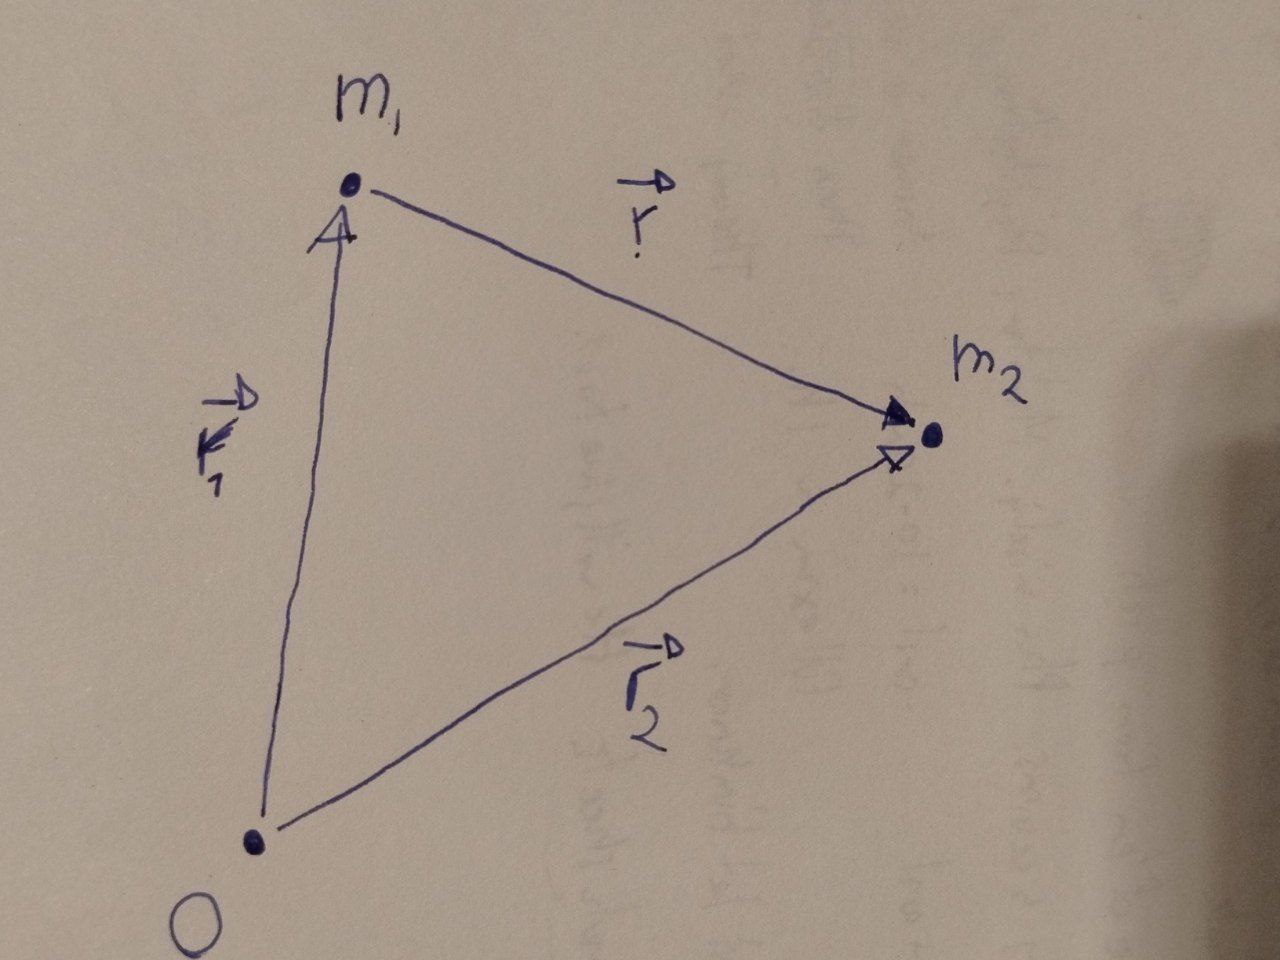
\includegraphics[width=\linewidth]{imm/ei_to_new.jpg} 
    %\caption{Gravitational \\  interaction of two masses}
    \vspace{12pt}
\end{minipage}
\end{figure}
\begin{minipage}[t]{0.48\textwidth}
    \vspace*{0pt} 
      We got two masses, $ m_{1}, m_{2} $, the origin, O, of the RF. \\ Each mass' position is identified by its own position vector.
	\begin{gather*}
\vec{r} = \vec{r}_{1}+\vec{r}_{2} \\
\vec{F}_{21}= - \frac{Gm_{1}m_{2}}{r^{2}} \hat{r} \\
\text{with } \hat{r} = \frac{\vec{r}}{|\vec{r}|}
	\end{gather*}
	   so, we see that m\textsubscript{2} is attracted. \\
	   P.S. $G = 6.67\times10^{-11} \frac{Nm^{2}}{kg^{2}} $
\end{minipage}

Introducing the second law of dynamics in the study, we have
\begin{gather*}
m_{2}\vec{a}_{2} = \vec{F}_{21} = - \frac{Gm_{1}m_{2}}{r^{2}} \hat{r} \\
\text{simplifying } m_{2} \text{ we obtain} \\
\vec{a}_{2} = - \frac{Gm_{1}}{r^{2}} \hat{r}  
\end{gather*}
We can express \textbf{a}\textsubscript{2} as 
\begin{gather*}
	\vec{a}_{2} = - \nabla \phi \text{ Gradient of the Gravitational Potential} \\
	\phi = - \frac{Gm_{1}}{r} \\
	\nabla^{2} \phi = -4\pi G \rho
\end{gather*}

We will use the Minkowski metric tensor 
\begin{equation}
	\eta_{\mu\nu} =
	\begin{pmatrix}
		-1 & 0 & 0 & 0 \\
		0 & +1 & 0 & 0 \\
		0 & 0 & +1 & 0 \\
		0 & 0 & 0 & +1 
	\end{pmatrix}
\end{equation}
 We will see also other symbols, like the Kristoffel one, or the Richie Tensor... \\
 But in the end the central goal is to derive the \emph{Einstein Equation}:
\begin{equation}
R_{\mu\nu} = \frac{1}{2} g_{\mu\nu}R = 8\pi G T_{\mu\nu}
\end{equation}

In GR particles move freely along \emph{straight lines} of a curved space-time. These are called \emph{geodesics}.

\paragraph{Example}
Two chalks, one on the desk, the other is launched in the air. Which one is accelerated?
From a GR perspective, the one in the air is moving along a geodesic, so it is the one moving freely, while the other is stopped from doing that by some interference/force. \\
In GR gravity is \emph{not} a force. 

\chapter{Math tools}
\section{A recap of SR}
\textbf{Lecture 2}
We will develop some of the necessary math on this framework. \\
Let's look at the Galilean Relativity. \\
Newtonian dynamics is based on three principles
\begin{enumerate}
	\item inertia
	\item $\vec{F} = m \vec{a}$
	\item action-reaction
\end{enumerate}
The first says something like \emph{An object at rest remains at rest, and an object in motion remains in motion at constant speed and in a straight line unless acted on by an unbalanced force}. \par
The second one says:
\[
	(2): \vec{F} = 0 \implies \vec{a} = 0 \implies (1)
\]

So, it seems the first principle is contained by the second, but we know that $\vec{F} = m \vec{a} $ is valid only in Inertial Frames (IF). \par
\paragraph{Galilean Relativity:} all the laws of \emph{mechanics} take the same form in every IF. (You can not distinguish two IF just by doing experiments.) \par
\begin{figure}
\begin{minipage}[t]{0.4\textwidth}
    \vspace*{0pt} 
    \centering
    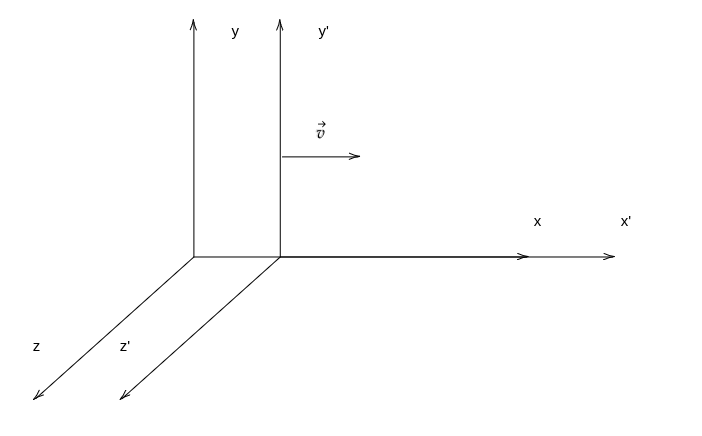
\includegraphics[width=\linewidth]{imm/galileianboost.png} 
    %\caption{G. Boost}
\end{minipage}

\end{figure}
\begin{minipage}[t]{0.4\textwidth}
    \vspace*{0pt}
    $
    \begin{cases}
    x' = x - vt \\
    y' = y \\
    z' = z \\
    t' = t
    \end{cases}$ \par
      $t = t' = 0 \implies O = O'$
\end{minipage} 
\bigskip

Taking the first derivative:
\begin{equation}
\begin{cases}
v_{x}' = v_{x} - v \\
v_{y}' = v_{y} \\
v_{z}' = v_{z} \\
\end{cases} \text{and for the second derivative: } \\
\begin{cases}
a_{x}' = a_{x} \\
a_{y}' = a_{y}\\
a_{z}' = a_{z}
\end{cases} \implies \vec{a}' = \vec{a}
\end{equation}
so also $\vec{F}' = \vec{F}$. And if \emph{m} is independent on the frame, we got
\begin{equation}
\vec{F}'=m \vec{a}' = \vec{F} = m \vec{a}
\end{equation}
\bigskip

Then there are Maxwell equations, people thanks to them find that EM-waves propagates with speed \emph{c} in the void. \par
But they found also that these equations were not invariant in Galilean Boosts. \par
Things started to go better when the idea of a preferred IF was ditched and Einstein decided to use Lorentz Transformations.\par

There are two postulates: \par
\begin{itemize}
	\item \emph{Relativity principle}: same as before but with \emph{physics} instead of \emph{mechanics}. \textbf{All the laws of physics ...}
	\item \emph{Speed of light}: in every IF, light propagates with constant speed, \emph{c}.
\end{itemize}
So we see that Galilean transformation become inconsistent with this, meanwhile stays valid for $\vec{v} \ll \vec{c}$.\par
As mentioned before, updated version of G. Boosts are Lorentz transformations (or Lorentz Boosts.)
\begin{equation}
\begin{cases}
	x' = \frac{x-vt}{\sqrt{1-(\frac{v}{c})^{2}}} \\
	y' = y \\
	z' = z \\
	t' = \frac{t- \frac{vx}{c^{2}}}{\sqrt{1-(\frac{v}{c})^{2}}}
\end{cases}
\end{equation}

To ensure the L.T. Is consistent we can perform three checks:
\begin{itemize}
	\item $v \ll c$
	\item v = 0
	\item dimensional check
\end{itemize}
People use a notation to make the L.T. easier to write: $\gamma(v) \equiv \frac{1}{\sqrt{1-(\frac{v}{c})^{2}}} $, so it becomes
\begin{equation}
\begin{cases}
x' = \gamma (x-vt) \\
y' = y \\
z' = z \\
t' = \gamma (t- \frac{vx}{c^{2}})
\end{cases}
\end{equation}

What happens to the transformation of velocity is: (v is fixed) 
\begin{equation}
\begin{cases}
dx' = \gamma(dx -vdt) \\
dy' = dy \\
dz' = dz \\
dt' = \gamma \left(dt - \frac{v dx}{c^{2}}\right)
\end{cases}
\end{equation}
 so 
\begin{equation}
\begin{cases}
 v_{x}' = \frac{dx'}{dt'} \\
 v_{y}' = \frac{dy'}{dt} = \frac{dy}{\gamma \left(dt - \frac{vdx}{c^{2}}\right)} = \frac{v_{y}}{\gamma \left(1- \frac{v v_{x}}{c^{2}}\right)} \\
v_{z}' = \frac{dz'}{dt} = ...
\end{cases}
\end{equation}
So we see that space-time changes also along other axes.\par

Now let's talk about space-time and its parts.

\paragraph{Space-time} space-time is a manifold. For now it is a collection of (t,x,y,z), four dimensional set of all the possible values of the coordinates.
\paragraph{Event} a point of space-time.
\paragraph{World line} path of a particle in space-time.

\begin{figure}
\centering
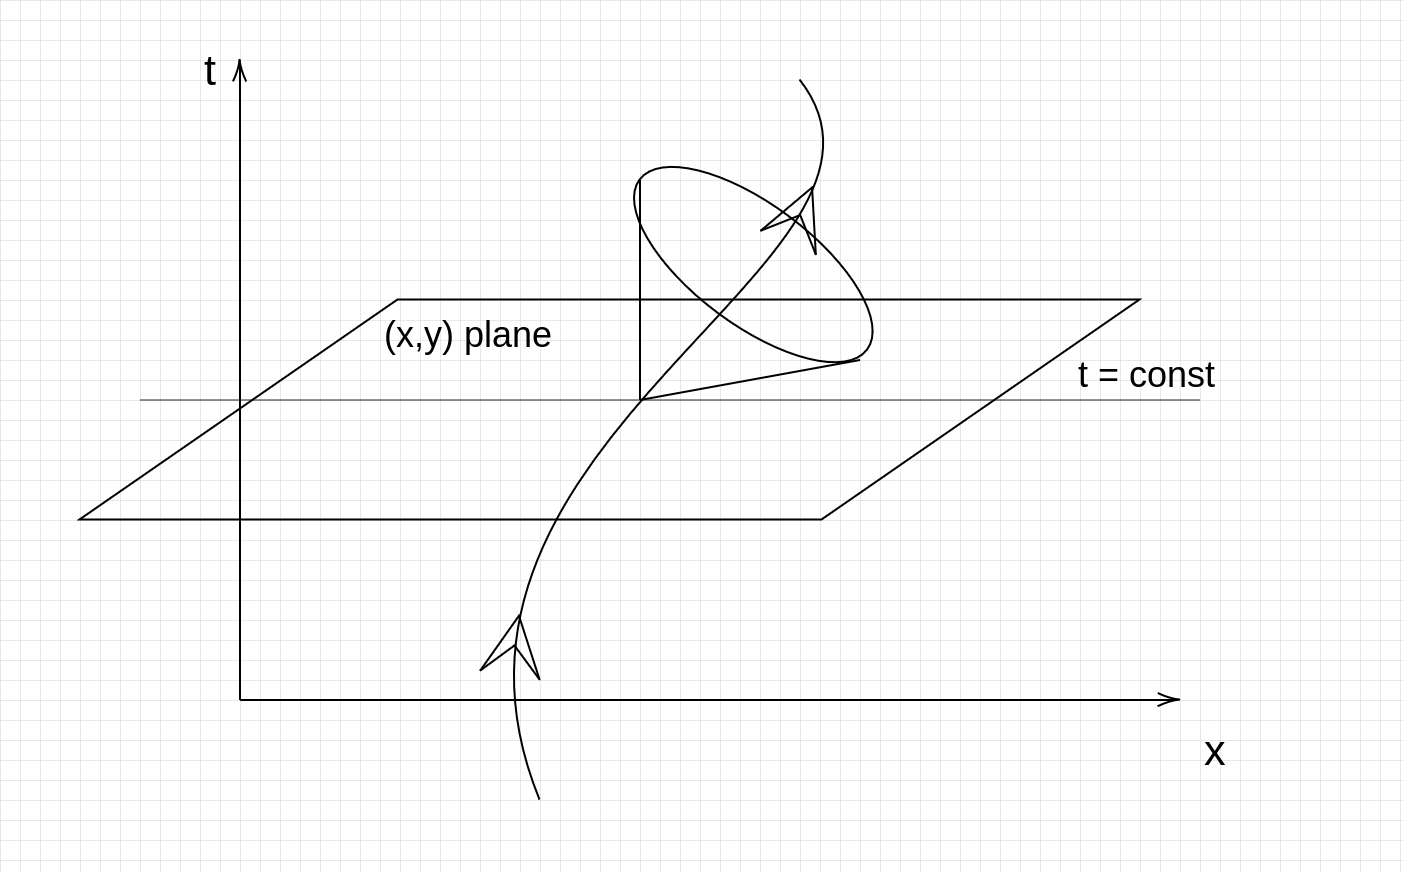
\includegraphics[width=\linewidth]{imm/WLLC.png}
\caption{LL of a particle which moves forward in time, we see also a light cone}
\label{mm:WLLC}
\end{figure}

There is no notion of absolute time anymore, because now it is dependent on the frame. 
Regarding the light-cone, after the event on the ( x,y ) plane, the particle can move \emph{only} inside the light-cone, in the appropriate direction (time forward).

Now let's talk about \textbf{Clock Synchronization.} \par
It is kinda easy if in in IF. In GR it is quite subtle instead. \par

\paragraph{Example:} Be me in Origin of a RF watching my clock (A). How to define \emph{t} at another generic location (B)??

\begin{figure}
\centering
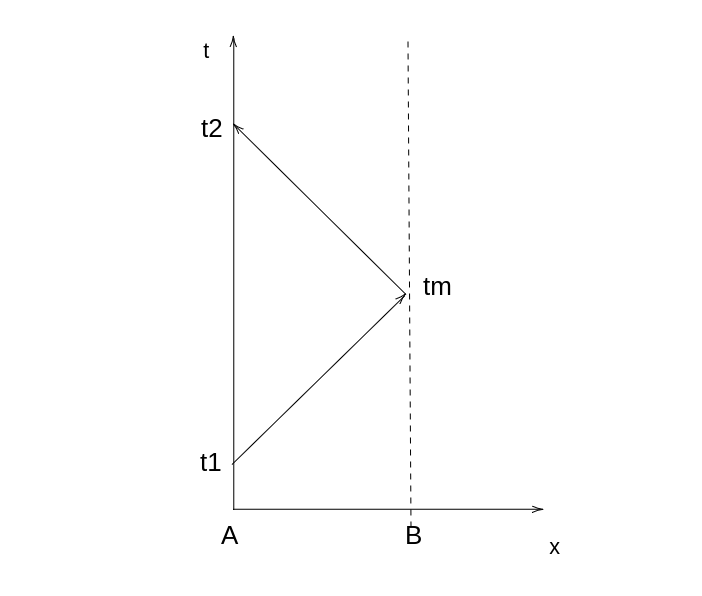
\includegraphics[width=\linewidth]{imm/segnale.png}
\caption{Reception and send of the signal}
\label{imm:segnale.png}
\end{figure}

I send a light ray at time \emph{t\textsubscript{1}} to B. I get the answer on \emph{t\textsubscript{2}}. There is symmetry between the two trajectories so \[
t_{m} = \frac{ t_{1} + t_{2} }{2}. 
\]
I say to my friend on B: "set your clock to t\textsubscript{m} when you receive the signal."
So, following this methodology, each point could have its own clock.

\paragraph{Proper time:} How to define proper time? \\
\emph{t} is the time coordinate. Let's introduce the metric tensor:
\begin{equation}
	\text{the Minkowski metric tensor: } \eta_{\mu \nu } = \begin{pmatrix}
	-1 & 0 & 0 & 0 \\
	0 & 1 & 0 & 0 \\
	0 & 0 & 1 & 0 \\
	0 & 0 & 0 & 1
	\end{pmatrix} 		
\end{equation}
for a Lorentz Transformation if I have 2 events E,F.
\begin{gather*}
	\text{Frame 1: } x_{F}^{\mu } = \left( t_{F}, x_{F}, y_{F}, z_{F} \right)\\
	x_{E} = \left( ... \right) \\
	\text{Frame 2: } x_{F}^{\mu' } = \left( t_{F'}, x_{F'}, y_{F'}, z_{F'} \right) \\
	x_{E}^{\mu' } = \left( ... \right)	 
\end{gather*}
same events in 2 different frames. \\
A Lorentz Transformation cornets these two events.

Be $\Delta s^{2}$ the Lorentz Invariant separation between E-F.
\begin{gather*}
\Delta s^{2} = -c \left( t_{F}-t_{E} \right)^{2} + \left( x_{F}- x_{E} \right)^{2} + \left( y_{F}-y_{E} \right)^{2} + \left( z_{F}-z_{E} \right)^{2} =\\
= -c (t_{F'}-t_{E'})^{2}  + (x_{F'}- x_{E'})^{2}  + (y_{F'}-y_{E'})^{2}  + (z_{F'}-z_{E'})^{2} \\
\Delta s^{2} = \eta_{\mu \nu } \Delta x^{\mu } \Delta x^{\nu } \\
\text{From this point we set } c = 1 \text{ just a rescaling} \\
\text{we have defined } \Delta x^{\mu } \equiv x_{F}^{\mu} - x_{F}^{\mu }, \text{with } \mu = 0,1,2,3.
\end{gather*}

So, repeating for clarity, the Lorentz Invariant separation is
\begin{equation}
\Delta s^{2} = \eta_{\mu  \nu } \Delta x^{\mu } x^{\nu } = \eta_{\mu'\nu'} \Delta x^{\mu '} \Delta x^{\nu'}
\end{equation}
Minkowski metric tensor does not change form if we change coordinates (Cartesian coordinates, meanwhile if we use like polar ones it changes for obvious reasons.) \par

if 
\begin{align*}
	\Delta s^{2} & > 0 \text{space-like separation} \\
		     &< \text{time-like, (it could be an actual LL for a massive particle)} \\
		     &= \text{light-like or null}
\end{align*}

Now we can define the \emph{proper time} as
\begin{equation}
	\Delta \tau^{2} \equiv - \Delta s^{2} \text{ or } \Delta \tau^{2} = - \eta_{\mu  \nu }\Delta x^{\mu } \Delta x^{\nu }
\end{equation}
So, if the proper time is \emph{positive} it is time-like.

If the segment \textbf{EF} marks the begin and end of the trajectory of a massive particle, $\Delta  \tau $, proper time, is the time elapsed on a clock sitting on a RF that moves with constant speed between E and F.
\\
Int the moving frame $\Delta \tau = \Delta t_{*}$ where \emph{t\textsubscript{*}} is the time coordinate of the moving frame. 
In a frame where I'm at rest this is how $\Delta t^{2}$ changes:
\begin{equation}
\Delta  \tau^{2} = + \Delta t^{2} - \Delta x^{2} - \Delta y^{2}- \Delta z^{2}.
\end{equation}

\section{Lecture 3}

The meaning of the Lorentz Invariant is that \textbf{events}, like $\left( E,F \right)$ exist before I define coordinates. It is a property of the two events.

So to recap what we did in the last lecture, be:
\begin{equation}
x_{E}^{\mu } \text{ and } x_{E}^{\mu'}
\end{equation}

\begin{figure}[ht]
\centering
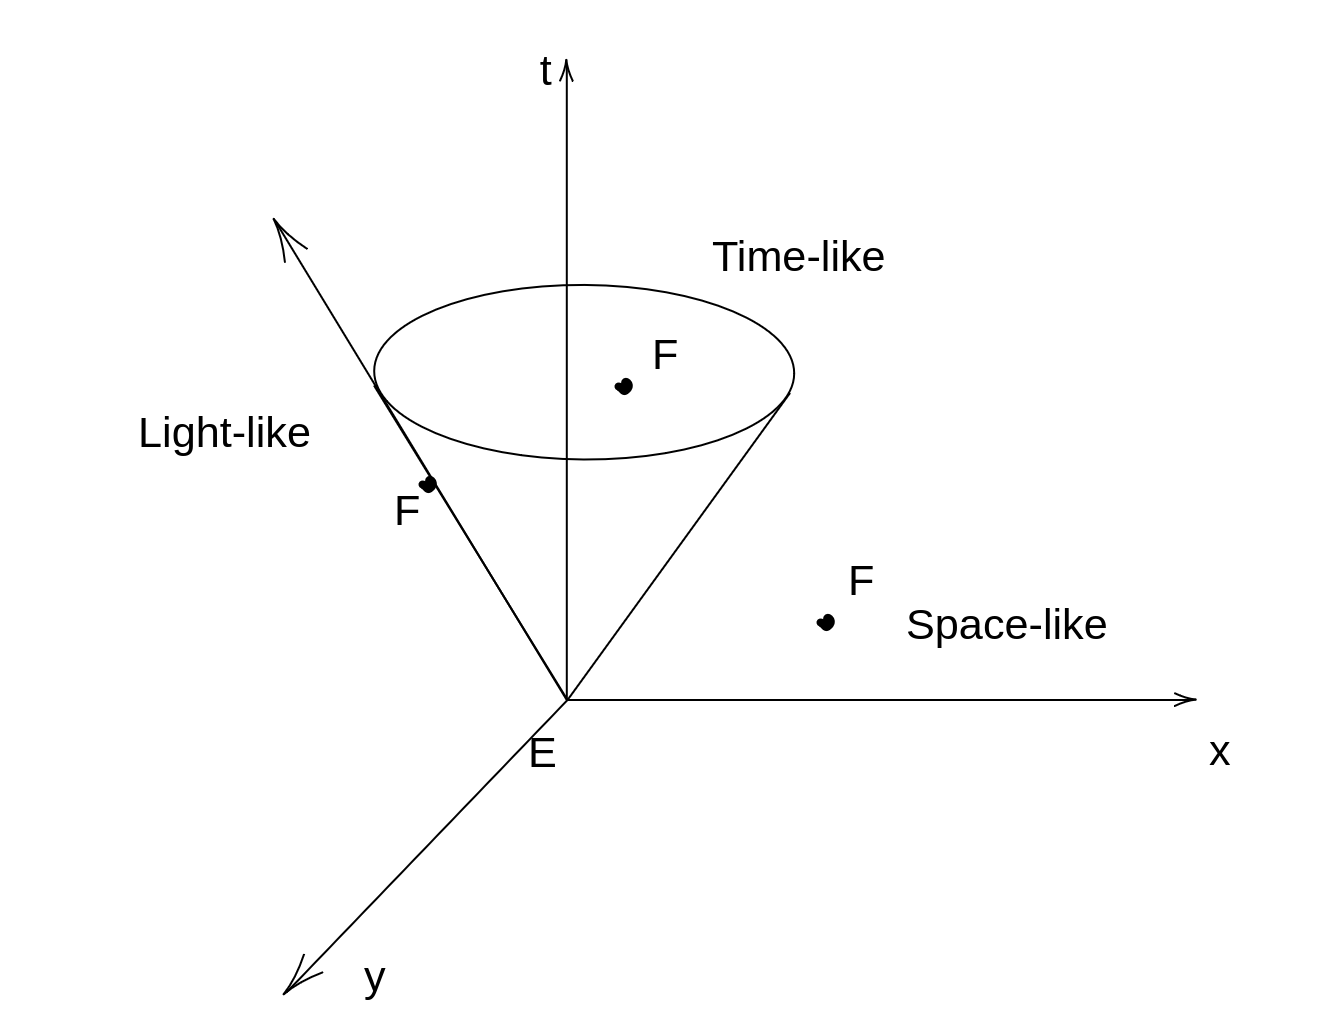
\includegraphics[width=\linewidth]{imm/lightcone.png}
\caption{Given event E, the separation \textbf{EF} could be of different types based on the position respect the light cone}
\label{imm:lightcone}
\end{figure}

If I have two events and computing $\Delta \tau $ gives a positive result, the separation is \textbf{time-like}.
This means that they could be on the WL of a massive particle moving at constant speed.

\paragraph{Physical meaning of $\Delta \tau $}
It's the time elapsed on a clock of the observer moving between E and F at constant speed.

This means that if I compute $\Delta \tau $ on the frame where the observer it is at rest, i get \[
\Delta \tau = \Delta t'
\]

Lets do an example:
\paragraph{Example}
\begin{figure}
\centering
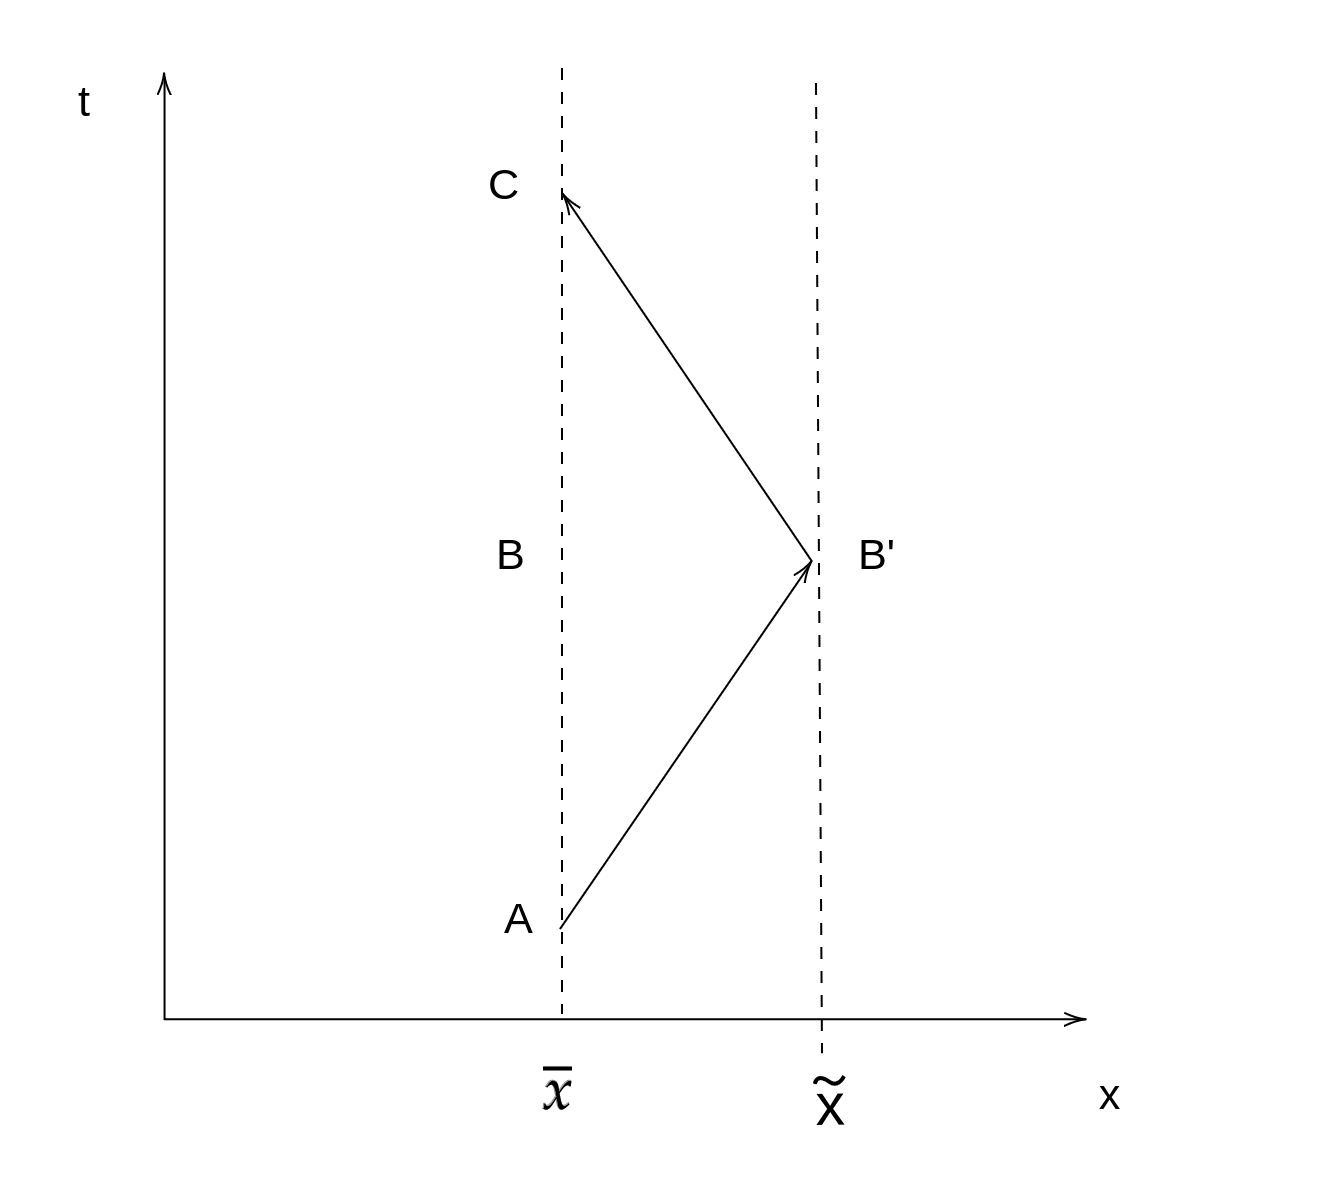
\includegraphics[width=\linewidth]{imm/examplelec3.png}
\caption{It is like the twin paradox.}
\label{imm:examplelec3}
\end{figure}

In fig. \ref{imm:examplelec3} we see the straight line \textbf{ABC} that is the WL of a object not moving. 
Computing its proper time will be:
\begin{equation}
\Delta \tau_{ABC} = \left( t_{c}-t_{A} \right)
\end{equation}
But for the other WL, of a object moving at constant speed between \textbf{AB'} and \textbf{B'C}, first thing first, we see that
\begin{gather*}
t_{B} = t_{B'} \\
\text{ and so } \\
\Delta \tau_{AB'C} = 2 \sqrt{\left( t_{B} - t_{A} \right)^{2} - \left( \tilde{x} - \bar{x} \right)^{2}} = \Delta \tau_{ABC} \sqrt{1 - \left( \frac{v}{c}  \right)^{2}} \\
\implies \Delta \tau_{AB'C} < \Delta \tau_{ABC}
\end{gather*}

This means that I have the longest \textbf{proper time} when I don't move.

We can do one more generalization: by parametrize the WL with a quantity $\lambda $ we get
\begin{gather*}
x^{\mu }\left( \lambda  \right) \\
\Delta \tau = \int \sqrt{- \eta_{\mu \nu } \frac{dx^{\mu }}{d\lambda } \frac{dx^{\nu }}{d\lambda }} d\lambda \text{ that is a time like trajectory. }
\end{gather*}

Enough with proper time.

\subsection{Tensor Calculus}
Be a Lorentz Group, we want to look for the transformations.
\begin{equation}
x^{\mu } \to x^{\mu'} = \Lambda^{\mu'}_{\mu } x^{\mu }
\end{equation}
we see that it is a linear transformation. An example to see better what are we doing could be
\begin{equation}
x^{0'} = \Lambda^{0'}_{0}x^{0} + \Lambda^{0'}_{1}x^{1} + \Lambda^{0'}_{2}x^{2} + \Lambda^{0'}_{3}x^{3}
\end{equation}
What we need to know is that $\Lambda^{\mu'}_{\mu }$ is a constant matrix.

We see that $\Lambda $   is a constant matrix.

We want to find linear transformations such that 
\begin{equation}
\Delta s^{2} = \eta_{\mu \nu } \Delta x^{\mu }\Delta x^{\nu } = \eta_{\mu' \nu'} \Delta x^{\mu'}\Delta x^{\nu'}
\end{equation}
So the Lorentz Invariant is still invariant. (WTF)

Now, because a SR property: if I move from IF to another, $\eta$ is still unchanged. So \[
\eta_{\mu \nu } = \eta_{\mu' \nu'}
\]

We have to say that Minkowski assumes cartesian coordinates.

The question now is: What trivial transformations leave $\Delta s^{2}$ unchanged?

\paragraph{Translations}
\begin{gather*}
\eta_{\mu  \nu }\Delta x^{\mu }x^{\nu } = \eta_{\mu' \nu'}\left( \Lambda^{\mu'}_{\mu }\Delta x^{\mu } \right) \left( \Lambda^{\nu'}_{\nu }\Delta x^{\nu } \right) \\
\implies \eta_{\mu  \nu } = \eta_{\mu' \nu'} \Lambda^{\mu'}_{\mu }\Lambda^{\nu'}_{\nu } \\
\text{ this obviously needs to be valid } \forall \Delta x^{\mu } \\
\text{ an alternative notation could be } \eta = \Lambda^{T} \eta \Lambda \\
\end{gather*}
We will use just the first notation, because we need to get good at tensors.

To be more concrete:
\begin{equation}
\Lambda^{\mu'}_{\mu } = \begin{pmatrix}
\Lambda^{0'}_{0} & \Lambda^{0'}_{1} & \Lambda^{0'}_{2} & \Lambda^{0'}_{3} \\
\Lambda^{1'}_{0} & ... & ... & ... \\
\Lambda^{2'}_{0} & ... & ... & ... \\
\Lambda^{3'}_{0} & ... & ... & ...
\end{pmatrix} 
\end{equation}

\paragraph{Rotations} 


Rotations are a kind of transformation of the type:
\begin{gather*}
x_{i'} = R_{i i'} x_{i} \\
\text{ or } R^{T} \mathbb{I} R = \mathbb{I} \\
\text{ with } RR^{T} = R^{T}R = \mathbb{I}
\end{gather*}

it could be something like
\begin{equation} \Lambda^{\mu'}_{\mu } = 
\begin{pmatrix}
cosh \eta  & -sinh \eta   & 0 & 0 \\
-sinh \eta  & cosh \eta  & 0 & 0 \\
0 & 0 & 1 & 0 \\
0 & 0 & 0 & 1
\end{pmatrix} 
\end{equation}
this one is a boost along the $x$ direction. If we do some computing we find that 
\[
tanh \eta \equiv v
\]
so this is the same of the L.T. we saw last week. \par

Rotations do not change the time coordinate. The point was to tell what L.T. is in this language.

\paragraph{Vectors}


I have a generic vector, \textbf{do i need to  specify about the RF} where it is defined, so in a specific spacetime location? {\tiny yes} \par

In newtonian mechanics parallel vectors are the same because I can superpose them, I can move them around, also to use the parallelogram rule to get a sum. \par
$\implies$If I have 3D euclidean space there is no ambiguities about where i move my vectors.\par
\textbf{BUT} in a sphere:

\noindent
\begin{minipage}[t]{0.45\textwidth}
	\vspace*{0pt}
\tikzset{every picture/.style={line width=0.4pt}} %set default line width to 0.75pt        

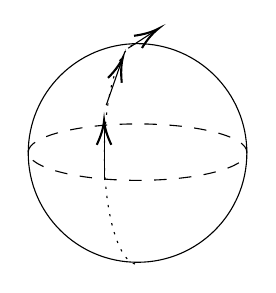
\begin{tikzpicture}[x=0.4pt,y=0.4pt,yscale=-1,xscale=1]
%uncomment if require: \path (0,300); %set diagram left start at 0, and has height of 300

%Shape: Circle [id:dp6654577831806846] 
\draw   (205.5,152.75) .. controls (205.5,98.21) and (249.71,54) .. (304.25,54) .. controls (358.79,54) and (403,98.21) .. (403,152.75) .. controls (403,207.29) and (358.79,251.5) .. (304.25,251.5) .. controls (249.71,251.5) and (205.5,207.29) .. (205.5,152.75) -- cycle ;
%Shape: Ellipse [id:dp25748828027722603] 
\draw  [dash pattern={on 4.5pt off 4.5pt}] (205.5,152) .. controls (205.5,137.92) and (249.71,126.5) .. (304.25,126.5) .. controls (358.79,126.5) and (403,137.92) .. (403,152) .. controls (403,166.08) and (358.79,177.5) .. (304.25,177.5) .. controls (249.71,177.5) and (205.5,166.08) .. (205.5,152) -- cycle ;
%Shape: Arc [id:dp3672101138168469] 
\draw  [draw opacity=0][dash pattern={on 0.84pt off 2.51pt}] (301.86,253.06) .. controls (286.41,249.01) and (274.25,206.07) .. (274.25,153.69) .. controls (274.25,100.16) and (286.95,56.49) .. (302.88,54.1) -- (304.25,153.69) -- cycle ; \draw  [dash pattern={on 0.84pt off 2.51pt}] (301.86,253.06) .. controls (286.41,249.01) and (274.25,206.07) .. (274.25,153.69) .. controls (274.25,100.16) and (286.95,56.49) .. (302.88,54.1) ;  
%Straight Lines [id:da2694092326525188] 
\draw    (274,177.5) -- (274,125.5) ;
\draw [shift={(274,123.5)}, rotate = 90] [color={rgb, 255:red, 0; green, 0; blue, 0 }  ][line width=0.75]    (21.86,-6.58) .. controls (13.9,-2.79) and (6.61,-0.6) .. (0,0) .. controls (6.61,0.6) and (13.9,2.79) .. (21.86,6.58)   ;
%Straight Lines [id:da8503547294122475] 
\draw    (276,109.5) -- (290.34,68.39) ;
\draw [shift={(291,66.5)}, rotate = 109.23] [color={rgb, 255:red, 0; green, 0; blue, 0 }  ][line width=0.75]    (21.86,-6.58) .. controls (13.9,-2.79) and (6.61,-0.6) .. (0,0) .. controls (6.61,0.6) and (13.9,2.79) .. (21.86,6.58)   ;
%Straight Lines [id:da6949662065564377] 
\draw    (295.88,58.1) -- (321.32,41.59) ;
\draw [shift={(323,40.5)}, rotate = 147.02] [color={rgb, 255:red, 0; green, 0; blue, 0 }  ][line width=0.75]    (21.86,-6.58) .. controls (13.9,-2.79) and (6.61,-0.6) .. (0,0) .. controls (6.61,0.6) and (13.9,2.79) .. (21.86,6.58)   ;

\end{tikzpicture}
\end{minipage}
\begin{minipage}[t]{0.48\textwidth}
    \vspace*{0pt} 
    I have this vector at the equator tangent to the surface. If I transport it to the pole i get a different vector.		
\end{minipage}
\bigskip

There are ambiguities. So in a non-flat space we need a \textbf{different} procedure. \par
A vector field is a map between:
\[
x^{\mu } \to v^{\mu }
\]
where $x^{\mu }$ is an event and $v^{\mu }$ is a vector. \par

Let's define: \textbf{Tangent space T\textsubscript{P}}.\par
Given an event $P$ we define the tangent space $T_{P}$ as all the vectors in $P$.\par

Instead of having spacetime we have a sphere.

\noindent
\begin{minipage}[t]{0.48\textwidth}
    \vspace*{0pt}
    

\tikzset{every picture/.style={line width=0.75pt}} %set default line width to 0.75pt        

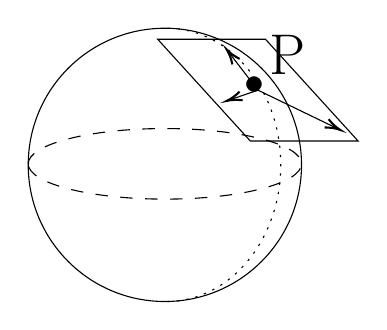
\begin{tikzpicture}[x=0.5pt,y=0.5pt,yscale=-1,xscale=1]
%uncomment if require: \path (0,300); %set diagram left start at 0, and has height of 300

%Shape: Circle [id:dp6654577831806846] 
\draw   (17.5,138.75) .. controls (17.5,84.21) and (61.71,40) .. (116.25,40) .. controls (170.79,40) and (215,84.21) .. (215,138.75) .. controls (215,193.29) and (170.79,237.5) .. (116.25,237.5) .. controls (61.71,237.5) and (17.5,193.29) .. (17.5,138.75) -- cycle ;
%Shape: Ellipse [id:dp25748828027722603] 
\draw  [dash pattern={on 4.5pt off 4.5pt}] (17.5,138) .. controls (17.5,123.92) and (61.71,112.5) .. (116.25,112.5) .. controls (170.79,112.5) and (215,123.92) .. (215,138) .. controls (215,152.08) and (170.79,163.5) .. (116.25,163.5) .. controls (61.71,163.5) and (17.5,152.08) .. (17.5,138) -- cycle ;
%Shape: Arc [id:dp3672101138168469] 
\draw  [draw opacity=0][dash pattern={on 0.84pt off 2.51pt}] (118.33,237.5) .. controls (163.51,236.96) and (200,192.96) .. (200,138.75) .. controls (200,84.76) and (163.8,40.88) .. (118.86,40.01) -- (117.5,138.75) -- cycle ; \draw  [dash pattern={on 0.84pt off 2.51pt}] (118.33,237.5) .. controls (163.51,236.96) and (200,192.96) .. (200,138.75) .. controls (200,84.76) and (163.8,40.88) .. (118.86,40.01) ;  
%Shape: Parallelogram [id:dp887464464445318] 
\draw   (111.1,48) -- (189,48) -- (255.9,121.5) -- (178,121.5) -- cycle ;
%Straight Lines [id:da3128101776711285] 
\draw    (183.5,84.75) -- (241.2,112.63) ;
\draw [shift={(243,113.5)}, rotate = 205.79] [color={rgb, 255:red, 0; green, 0; blue, 0 }  ][line width=0.75]    (10.93,-3.29) .. controls (6.95,-1.4) and (3.31,-0.3) .. (0,0) .. controls (3.31,0.3) and (6.95,1.4) .. (10.93,3.29)   ;
%Straight Lines [id:da05720579900710121] 
\draw    (183.5,84.75) -- (162.22,57.09) ;
\draw [shift={(161,55.5)}, rotate = 52.43] [color={rgb, 255:red, 0; green, 0; blue, 0 }  ][line width=0.75]    (10.93,-3.29) .. controls (6.95,-1.4) and (3.31,-0.3) .. (0,0) .. controls (3.31,0.3) and (6.95,1.4) .. (10.93,3.29)   ;
%Straight Lines [id:da5083189086137138] 
\draw    (183.5,84.75) -- (162.89,91.85) ;
\draw [shift={(161,92.5)}, rotate = 340.99] [color={rgb, 255:red, 0; green, 0; blue, 0 }  ][line width=0.75]    (10.93,-3.29) .. controls (6.95,-1.4) and (3.31,-0.3) .. (0,0) .. controls (3.31,0.3) and (6.95,1.4) .. (10.93,3.29)   ;

% Text Node
\draw (172,73.4) node [anchor=north west][inner sep=0.75pt]  [font=\Large]  {$\bullet $};
% Text Node
\draw (190,43) node [anchor=north west][inner sep=0.75pt]   [align=left] {{\huge P}};


\end{tikzpicture}

\end{minipage}
\begin{minipage}[t]{0.48\textwidth}
    \vspace*{0pt} 
	Define a plane tangent to the sphere only in $P$. All vectors that lie there $\in T_{P}$.    
\end{minipage}
\bigskip


$T_{P}$ is a \textbf{vector space}:
\[
	V,W \in T_{P} \implies \alpha V + \beta W, \left( \alpha , \beta \in \mathbb{R} \right) \in T_{P}
\]
So if there is a vector there is also the inverse vector.\par
Whenever i have a vector space, I can define infinite basis independently on the coordinate choice. The nUmber of elements in the basis is equal to the dimension of the space, in our case 4 elements.\par
Obviously if I define the basis its elements need to be Linearly Independent. 

\paragraph{Basis}
Given a generic vector $V \in T_{P}$, I can define $V$ regardless the coordinate system I'm using. So we can say \emph{meTaphorically} that $V$ exists before I define coordinates.\par

Be our basis:
\[
\hat{e}_{\left( \mu  \right)}, \text{ with } \mu = 0,1,2,3	
\]
those indices are label, does not mean "tensor". So my basis is made of \[
\hat{e}_{\left( 0 \right)}, \hat{e}_{\left( 1 \right)}, \hat{e}_{\left( 2 \right)}, \hat{e}_{\left( 3 \right)}
\]
Now we can talk about
\paragraph{Components}
given a generic vector $v$ 
\[
V = V^{0}\hat{e}_{\left( 0 \right)} + V^{1}\hat{e}_{\left( 1 \right)} + V^{2}\hat{e}_{\left( 2 \right)} + V^{3}\hat{e}_{\left( 3 \right)} =  V^{\mu }\hat{e}_{\left( \mu  \right) }
\]
using repeating indices we get the last equivalence.

$V^{\mu }$ are components of the vector $V$ in this specific frame. \par
In another frame $V^{\mu '}$ could not be the same:
\[
	V = V^{\mu }\hat{e}_{\left( \mu  \right)} = V^{\mu '}\hat{e}_{\left( \mu ' \right)}
\]

\textbf{Question:} how do components transform?
\paragraph{covariant vector}: is a math object whose components transform based on position
\[
V^{\mu '} = \Lambda^{\mu '}_{\mu }V^{\mu }
\]
These are not the only covariant vectors (?).

If you have a generic WL or path, you can parametrize the position by a $\lambda$ in this way:
\[
x^{\mu }\left( \lambda  \right)
\]
And taking its first derivative you get something similar to the four-velocity
\[
u^{\mu }\sim \frac{dx^{\mu }}{d\lambda }
\]
(I say similar because four-velocity is defined like $u^{\mu } = \frac{dx^{\mu }}{d\tau }$).

If I do a L.T. $x^{\mu }$ will change but $\lambda $ won't.
\[
u^{\mu '} = \Lambda^{\mu '}_{\mu }u^{\mu }
\]
I can get a more general definition of what a vector is by following this procedure:
choose basis $\to$ find components $\to$ study how components change if i change position or basis.

\paragraph{Second definition}: Transformation of the basis vectors. The question is "how to relate $\hat{e}_{\left( \mu  \right)}$ to $\hat{e}_{\left( \mu ' \right)}$?"

We will take advantage of \textbf{invariance}. 
\[
V = V^{\mu }\hat{e}_{\left( \mu  \right) } = V^{\mu '}\hat{e}_{\left( \mu ' \right)} = \left( \Lambda^{\mu '}_{\mu }V^{\mu } \right)\hat{e}_{\left( \mu ' \right)}
\]
That's possible \textbf{only} if $\hat{e}_{\left( \mu  \right)} = \Lambda^{\mu '}_{\mu }\hat{e}_{\left( \mu ' \right)}$.

An inverse of LT it is also a LT, so
\begin{gather*}
\Lambda^{\mu '}_{\mu }\Lambda^{\mu }_{\nu '} = \delta^{\mu '}_{\nu '} \\
\Lambda^{\mu }_{\mu '}\Lambda^{\mu '}_{\nu } = \delta^{\mu }_{\nu }	
\end{gather*}
Those are Kroneker's delta and they are an Identity matrix.

Now we can study how basis vectors change.
\begin{gather*}
\hat{e}_{\left( \mu  \right)} = \Lambda^{\mu '}_{\mu }\hat{e}_{\left( \mu ' \right)} \\
\Lambda^{\mu }_{\nu '}\hat{e}_{\left( \mu  \right)} = \Lambda^{\mu '}_{\mu }\Lambda^{\mu }_{\nu '} \hat{e}_{\mu '} \\
\Lambda^{\mu }_{\nu '}\hat{e}_{\left( \mu  \right)} = \delta^{\mu '}_{\nu '}\hat{e}_{\left( \mu ' \right)} \\
\Lambda^{\mu }_{\nu '}\hat{e}_{\left( \mu  \right)} = \hat{e}_{\left( \nu ' \right)} \\ 
\text{ so } \hat{e}_{\left( \nu ' \right)} = \Lambda^{\mu }_{\nu '}\hat{e}_{\left( \mu  \right)}
\end{gather*}
\section{Lecture 4}

\subsubsection{Brief recap of lec3}
We defined vectors
\begin{itemize}
	\item localized at each spacetime point
	\item for each event P we defined the tangent space $T_{P}$
	\item there is linear combination inside $T_{P}$
	\item it has a basis
	\item Vectors and basis transform under LT Group.
\end{itemize}

\subsubsection{Dual vectors}
Using old terminology they are covariant, so with lower indices. Meanwhile contravariant do have upper indices.

Let's start with defining the \textbf{dual space} of a vector space:
\emph{Given a vector space (for concreteness T\textsubscript{P})}, we define the \textbf{dual space} $T_{P}^{*}$ as the space of linear maps between $T_{P}$ and $\mathbb{R}$.

\paragraph{Example}
Being $\omega  \in T_{P}^{*}$, $V \in T_{P}$ then
\[
	\omega \left( V \right) \in \mathbb{R}
\]
Linearity tells me that 
\[
\omega \left( \alpha V + \beta  W \right) = \alpha \omega \left( V \right) + \beta \omega \left( W \right)
\]

\paragraph{1\textsuperscript{st} statement}: The dual space is a vector space.
\[
	\left( \alpha \omega  + \beta \eta  \right)\left( v \right) = \alpha \omega \left( v \right) + \beta \eta \left( v \right)
\]
\paragraph{2\textsuperscript{nd} statement}: What is the dual of the dual?
\[
	\left( T_{P}^{*} \right)^{*} = T_{P} \implies v\left( \omega  \right) = \omega \left( v \right) \in \mathbb{R}
\]

\paragraph{Basis for T\textsubscript{P}\textsuperscript{*}}: $\hat{o}^{\left( \mu  \right)}$. \\
How to define this? Definition is
\[
\hat{o}^{\left( \mu  \right)}\left( \hat{e}_{\left( \nu  \right)} \right) \equiv \delta^{\mu }_{\nu }
\]
Now let's see if we can get how dual vectors work with vectors.
If I have:
\begin{itemize}
	\item generic item of $T_{P}$: $V = V^{\nu }\hat{e}_{\left( \nu  \right)}$
	\item generic item of $T_{P}^{*}: \omega = \omega_{\mu }\hat{o^{\left( \mu  \right)}}$ 
\end{itemize} 

I can compute:
\begin{gather*}
\omega \left( v \right) = \omega_{\mu }\hat{o}^{\left( \mu  \right)}\left( v^{\nu }\hat{e}_{\left( \nu  \right)} \right) =  \\
= \omega_{\mu }v^{\nu }\hat{o}^{\left( \mu  \right)}\left( \hat{e}_{\left( \nu  \right)} \right) = \omega_{\mu } v^{\nu } \delta^{\mu}_{\nu } = \omega_{\mu }v^{\mu }
\end{gather*}

\noindent\fbox{\begin{minipage}{\textwidth}
Once we know this we can do an \textbf{exercise}: show the way $\omega_{\mu '}$ transform.
What to do is to start from $\Lambda $ equality.\\
\end{minipage}} \\

What is the example of a dual vector? \\
\[
A_{\mu '} = \Lambda_{\mu }^{\mu '} A_{\mu }
\]
the gradient is a beautiful example of a \emph{dual vector}.
\[
A_{\mu } = \frac{\partial\phi }{\partial x^{\mu }} \text{  ;   } A_{\mu '} = \frac{\partial\phi }{\partial x^{\mu '}}
\]
This is useful to define LTs, in this way
\[
\frac{\partial\phi }{\partial x^{\mu '}} = \frac{\partial\phi }{\partial x^{\mu }} \frac{\partial x^{\mu }}{\partial x^{\mu '}} \to A_{\mu '} = \frac{\partial x^{\mu }}{\partial x^{\mu '}}A_{\mu }
\]
the LT is the last partial derivative. \\

There is a \emph{more compact} notation tho write partial derivatives that is
\[
\partial_{\mu } \phi \equiv \frac{\partial\phi }{\partial x^{\mu }}
\]

\subsection{Tensors}

Tensors are generalization of dual vectors and vectors. \\
They are \emph{multilinear maps}, i.e. functions of several variables and linear for all of them. For each tensor of \emph{rank} (k,l), we have
\[
T_{P}^{*}\times \ldots \times T_{P}^{*} \times T_{P}\times \ldots \times T_{P} \to \mathbb{R} \]
Where each dual vector space is present \textbf{k}-times, and vector space \textbf{l}-times.

Now let's see what is multilinearity on the combat field.

\noindent\fbox{
	\begin{minipage}{0.95\textwidth}
	Be a (1,1) tensor:
	\begin{itemize}
		\item $\alpha , \beta , \gamma , \delta \in \mathbb{R}$
		\item $\omega , \eta  \in T_{P}^{*}$
		\item v,w $\in $ T\textsubscript{P}
	\end{itemize}
	Given these we have
	\begin{equation}
	T\left( \alpha \omega + \beta \eta , \gamma v + \delta w \right) = \\
	= \alpha \gamma T\left( \omega , v \right) + \beta \delta T\left( \eta , w \right) + \alpha \delta T\left( \omega , w \right) + \beta \gamma T\left( \eta ,v \right)
	\end{equation}

\end{minipage}}

Once we have this general definition, let's take one step back:
\begin{itemize}
	\item Scalar $\to$ (0,0) tensor
	\item Vector $\to$ (1,0) tensor
	\item Dual vector $\to$ (0,1) tensor
\end{itemize}

\subsubsection{Tensor product}
Be:
\begin{itemize}
	\item T, rank (k,l) tensor
	\item S, rank (m,n) tensor
\end{itemize} 
We want to understand the action of $\otimes$. \\
So we know that $T\otimes S$ outputs (k+m, l+n) tensor. In particular,
\begin{gather*}
	T\otimes S \left[\omega^{\left( 1 \right)}, \ldots, \omega^{\left( k \right)}, \omega^{\left( k+1 \right)}, \ldots , \omega^{\left( k+m \right)}, v^{\left( 1 \right)}, \ldots , v^{\left( l \right)}, v^{\left( l+1 \right)}, \ldots , v^{\left( l+n \right)}\right] \equiv \\
	\equiv T\left( \omega^{\left( 1 \right)}, \ldots , \omega^{\left( k \right)}, v^{\left( 1 \right)}, \ldots , v^{\left( l \right)} \right) \times S\left( \omega^{\left( k+1 \right)}, \ldots , \omega^{\left( k+m \right)}, v^{\left( l+1 \right)}, \ldots , v^{\left( l+n \right)} \right) \\
	\implies T \otimes S \neq S \otimes T
\end{gather*}
so tensors do not commute.\\

\subsubsection{Basis for a tensor}
Let \emph{T} be a generic tensor with rank (k,l), \emph{basis} is given by
\[
\hat{e}_{\left( \mu_{1} \right)} \otimes \ldots \otimes \hat{e}_{( \mu_{k})} \otimes  \hat{o}^{\left( \nu_{1} \right)} \otimes \ldots \otimes \hat{o}^{(\nu_{l})}
\]

 A tensor can be written as 
 \[
 T = T^{\mu_{1}, \ldots , \mu_{k}}_{\nu_{1}, ..., \nu_{l}} \left( \hat{e}_{\left( \mu_{1} \right)} \otimes \ldots  \right) = T^{\mu_{1}^{'}, \ldots , \mu_{k}^{'}}_{\nu_{1}^{'}, \ldots , \nu _{l}^{'}}\left( \hat{e}_{\left( \mu_{1}^{'}  \right)} \otimes \ldots  \right)
 \]
So the tensor is always the same, the thing that changes is its components, because a change of RF I think.

We will often write the components instead of the actual tensor, but it is our convention to think they are equivalent.

This is how the components are related:
\begin{gather*}
\hat{e}_{\left( \mu ' \right)} = \Lambda^{\mu }_{\mu '} \hat{e}_{\left( \mu  \right)} \\
\hat{o}^{\left( \mu ' \right)} = \Lambda^{\mu '}_{\mu }\hat{o}^{\left( \mu  \right)} \\
\implies T = T^{\mu_{1}, \ldots , \mu_{k}}_{\nu_{1}, \ldots , \nu_{l}} \left( \Lambda^{\mu_{1}'}_{\mu_{1}} \hat{e}_{\left( \mu_{1}' \right)} \otimes \ldots  \right)
\end{gather*}
So we find, as result, that when I change frame
\begin{equation}
T^{\mu_{1}', \ldots , \mu_{k}'}_{\nu_{1}', \ldots , \nu_{k}'} = \Lambda^{\mu_{1}'}_{\mu_{1}} \ldots \Lambda^{\nu_{1}}_{\nu_{1}'} \ldots T^{\mu_{1}, ..., \mu_{k}}_{\nu_{1}, \ldots , \nu_{l}}
\end{equation}


\section{Lec 5}
\subsection{Transformations}
The goal is to find what is this $T^{\mu_{1}', \ldots , \mu_{k}'}_{\nu_{1}', \ldots , \nu_{l}'}= ?$.
\begin{equation}
T = T^{\mu_{1}, \ldots , \mu_{k}}_{\nu_{1, \ldots , \nu_{l}}} \left( \hat{e}_{\left( \mu_{1} \right)} \otimes \ldots  \right) = T^{\mu_{1}', \ldots , \mu_{k}'}_{\nu_{1}', \ldots , \nu_{l}'} \left( \hat{e}_{\left( \mu_{1}' \right)} \otimes \ldots  \right)
\end{equation}
I know two facts:
\begin{equation}
\begin{cases}
\hat{e}_{\mu '} = \Lambda^{\mu }_{\mu '} \hat{e}_{\left( \mu  \right)} \\
\hat{o}^{\mu '} = \Lambda^{\mu' }_{\mu } \hat{o}^{\mu } \\
\end{cases}
\end{equation}
and also the \emph{inverse.} \par

So i apply the Lambda transformation to each term of the basis and I get the following
\begin{equation}
T^{\mu_{1}', \ldots , \mu_{k}'}_{\nu_{1}', \ldots , \nu_{l}' } = \left( \Lambda^{\mu_{1}'}_{\mu_{1}} \ldots \Lambda^{\mu_{k}'}_{\mu_{k}} \right) \left( \Lambda^{\nu_{1}}_{\nu_{1}'} \ldots  \Lambda^{\nu_{l}}_{\nu_{l}'} \right) \left( T^{\mu_{1}, \ldots , \mu_{k}}_{\nu_{1}, \ldots , \nu_{l}} \right)
\end{equation}
that is something that was obvious by looking at indexes.

\subsection{Tensor Manipulations / Operations}
We defined $\left( k,l \right)$ vectors as a multilinear map from dual spaces and vector spaces to real numbers, but it is not only that. For example a $\left( 1,1 \right)$ tensor could be a map from vectors to vectors, in this way
\begin{equation}
V^{\mu } \to A^{\mu }_{\nu } V^{\nu }
\end{equation}
so if i do not saturate all the indices, i get a tensor of rank made by what remains. If we saturate, we get real numbers or (0,0) tensors.

There are some objects that are well known in flat spacetime.
\subsubsection{Particular Tensor in flat ST}
These are
\begin{itemize}
	\item $\eta_{\mu  \nu }$ metric, or metric tensor
	\item $\eta^{\mu \nu }$, inverse metric
	\item $\delta^{\mu }_{\nu }$, Kronecker's $\delta $
	\item $\epsilon_{\mu \nu \rho \delta }$, totally anti-symmetric tensor of Levi-Civita
\end{itemize}

This last one is defined:
\begin{equation}
\begin{cases}
+1 \text{ if } \left( 0,1,2,3 \right) \text{ or even permutations } \\
-1 \text{ if  odd permutations} \\
0 \text{ otherwise }
\end{cases}
\end{equation}

These are the only tensors of the flat spacetime that their components do not depend on the RF. \par

\subsubsection{Other operations}
\paragraph{Contraction} \[
	\left( k,l \right) \to \left( k-1, l-1 \right)
\]
Example: I have (3,2) tensor $T^{\mu \nu \rho }_{\delta \gamma } \to \left( 2,1 \right) ??$
We contract:
\[
	T^{\mu \colorbox{yellow}{$\nu$ } \rho  }_{\delta \colorbox{yellow}{$\gamma$} } \to T^{\mu  \colorbox{yellow}{$ \nu   $} \rho }_{\delta \colorbox{yellow}{$ \nu   $} } \equiv A^{\mu  \rho }_{\delta } 
\]

Obviously I can \emph{only} contract an upper with a lower index. \\
It is very important the order, and which indices we contract.
\[
T^{\mu  \colorbox{yellow}{$ \nu   $} \rho }_{\delta  \colorbox{yellow}{$ \nu   $} } \neq T^{\mu  \colorbox{yellow}{$ \nu   $} \rho }_{ \colorbox{yellow}{$ \nu   $} \delta  }
\]

What is the actual operation we perform?
\[
T^{\mu \nu \rho }_{\delta  \gamma } = \delta^{\gamma }_{\nu } T^{\mu  \nu \rho }_{\delta \gamma }
\]
\paragraph{Raising/Lowering Indices}
To raise we use $\eta^{\mu \nu }$, to lower $\eta_{\mu \nu }$.
\begin{gather*}
\eta^{\rho \alpha } T^{\mu \nu }_{\alpha \beta } \equiv T^{\mu  \nu  \rho }_{ \beta  } \\
\eta^{\rho \colorbox{yellow}{$ \beta   $} } T^{\mu \nu }_{\alpha \colorbox{yellow}{$ \beta   $} } \equiv T^{\mu \nu \colorbox{yellow}{$ \beta   $} }_{\alpha }
\end{gather*}
The order is important, and wring by hand one should be careful keeping the position moving up and down the indices. \par

Simple operations:
\begin{gather*}
V^{\mu } \to V_{\mu} = \eta_{\mu \nu } V^{\nu } \\
V_{\mu } \to V^{\mu } = \eta^{\mu \nu } V_{\nu }
\end{gather*}

\paragraph{Inner Product}
\[
	T_{P}\times T_{P} \to \mathbb{R}
\]
\[
	\left( V,W \right) \to \eta_{\mu \nu }V^{\mu }V^{\nu }
\]

\subsubsection{Symmetry Properties}
Let's consider a (0,2) tensor $T_{\mu \nu }$, or to be precise, its components.
It is symmetric? Anti-symmetric? Both? None?

A tensor is \emph{symmetric} if
\[
T_{\mu \nu } = T_{\nu  \mu }
\]
it is \emph{anti-symmetric} if
\[
T_{\mu  \nu } = - T_{\nu  \mu }
\]
It is \textbf{never} possible to have a tensor that is \emph{both}. But really possible that is \emph{none} of the above.

We can \emph{symmetrize} a tensor:
\[
T_{\left( \mu  \nu  \right)} = \frac{1}{2} \left( T_{\mu  \nu } + T_{\nu \mu } \right)
\]
We can \emph{anti-symmetrize} a tensor:
\[
	T_{[\mu  \nu ]} = \frac{1}{2} \left( T_{\mu \nu } - T_{\nu  \mu } \right)
\]
A tensor can be symmetric on all indices, so it \emph{totally symmetric}, or just on some indices, like two, three etc.
The general formula can be:
\[
T_{\left( \mu  \nu  \rho  \right)} = \frac{1}{3!} \left( T_{\mu  \nu  \rho } + \text{ all permutations } \right)
\]
For anti-simmetrizing odd permutations get the minus in front.

\subsubsection{Trace}
\[
x^{\mu }_{\mu }
\]
given a (1,1) tensor $\to \mathbb{R}$ by summing all indices.
For example the trace of metric tensor is 2.
Of Kronecker delta is 4.

\section{Lec 6}
\subsection{Energy \& momentum}
Since out goal is to get to the Einstein Equation, we know that in there there should be the \emph{energy momentum tensor} $T^{\mu \nu }$. \\
As always we will study everything for a flat space-time but it will be useful for non flat ones. \\
We already saw the four-velocity $u^{\mu}$:
\[
u^{\mu } \equiv \frac{d x^{\mu }}{d\tau }
\]
while the proper time is $\Delta \tau^{2} = - \eta_{\mu \nu }dx^{\mu }dx^{\nu }$. \\
We need to make clear that we are talking about a time-like space-time trajectory, so $\Delta s^{2}<0$. \\
Let's start with the WL of a single particle, this is specified by a map $\mathbb{R}\to M$, where $M$ is a manifold that represents spacetime. We usually think the path as a curve parameterized by $\lambda $ so $x^{\mu }\left( \lambda  \right)$. \\
We also use as parameter the $\tau $ so $x^{\mu }\left( \tau  \right)$, this has some advantages because maybe it could be easier to switch to four-velocity.
\begin{equation}
u^{\mu }u_{\mu } = u_{\mu }u^{\mu } = \eta_{\mu \nu } u^{\mu }u^{\nu } = -1
\end{equation}
By the way, four-velocity is what we need to find the \emph{four momentum}:
\begin{equation}
p^{\mu } \equiv m u^{\mu }
\end{equation}
where m is the rest mass that has the same values $\forall$ RF, and it's just a number.

So in rest frame (x',y',z'):

\noindent
\begin{minipage}[t]{0.48\textwidth}
    \vspace*{0pt}

\begin{tikzpicture}[x=0.3pt,y=0.3pt,yscale=-1,xscale=1]
%uncomment if require: \path (0,514); %set diagram left start at 0, and has height of 514

%Straight Lines [id:da944915482116456] 
\draw    (250.32,299.23) -- (250.32,32) ;
\draw [shift={(250.32,30)}, rotate = 90] [color={rgb, 255:red, 0; green, 0; blue, 0 }  ][line width=0.75]    (10.93,-3.29) .. controls (6.95,-1.4) and (3.31,-0.3) .. (0,0) .. controls (3.31,0.3) and (6.95,1.4) .. (10.93,3.29)   ;
%Straight Lines [id:da15966795743012707] 
\draw    (250.32,299.23) -- (594.16,299.23) ;
\draw [shift={(596.16,299.23)}, rotate = 180] [color={rgb, 255:red, 0; green, 0; blue, 0 }  ][line width=0.75]    (10.93,-3.29) .. controls (6.95,-1.4) and (3.31,-0.3) .. (0,0) .. controls (3.31,0.3) and (6.95,1.4) .. (10.93,3.29)   ;
%Straight Lines [id:da1019518678879453] 
\draw    (250.73,299.23) -- (96.56,422.08) ;
\draw [shift={(95,423.32)}, rotate = 321.45] [color={rgb, 255:red, 0; green, 0; blue, 0 }  ][line width=0.75]    (21.86,-6.58) .. controls (13.9,-2.79) and (6.61,-0.6) .. (0,0) .. controls (6.61,0.6) and (13.9,2.79) .. (21.86,6.58)   ;
%Straight Lines [id:da7761915086395399] 
\draw    (410.52,166.36) -- (410.52,41) ;
\draw [shift={(410.52,39)}, rotate = 90] [color={rgb, 255:red, 0; green, 0; blue, 0 }  ][line width=0.75]    (10.93,-3.29) .. controls (6.95,-1.4) and (3.31,-0.3) .. (0,0) .. controls (3.31,0.3) and (6.95,1.4) .. (10.93,3.29)   ;
%Straight Lines [id:da2518341020035201] 
\draw    (410.52,166.36) -- (558.87,166.36) ;
\draw [shift={(560.87,166.36)}, rotate = 180] [color={rgb, 255:red, 0; green, 0; blue, 0 }  ][line width=0.75]    (10.93,-3.29) .. controls (6.95,-1.4) and (3.31,-0.3) .. (0,0) .. controls (3.31,0.3) and (6.95,1.4) .. (10.93,3.29)   ;
%Straight Lines [id:da6843037394854449] 
\draw    (410.7,166.36) -- (344.51,223.76) ;
\draw [shift={(343,225.07)}, rotate = 319.07] [color={rgb, 255:red, 0; green, 0; blue, 0 }  ][line width=0.75]    (21.86,-6.58) .. controls (13.9,-2.79) and (6.61,-0.6) .. (0,0) .. controls (6.61,0.6) and (13.9,2.79) .. (21.86,6.58)   ;
%Shape: Free Drawing [id:dp9557143063465285] 
\draw  [line width=3] [line join = round][line cap = round] (410.85,166.25) .. controls (410.85,167.51) and (410.44,163.59) .. (410.85,162.46) .. controls (411.44,160.78) and (416.94,165.75) .. (410.85,170.04) .. controls (409.05,171.31) and (407.47,166.25) .. (405.46,166.25) ;
%Straight Lines [id:da5108630624179767] 
\draw [color={rgb, 255:red, 192; green, 40; blue, 40 }  ,draw opacity=1 ]   (411.99,165.5) -- (585.99,164.54)(412.01,168.5) -- (586.01,167.54) ;
\draw [shift={(594,166)}, rotate = 179.69] [color={rgb, 255:red, 192; green, 40; blue, 40 }  ,draw opacity=1 ][line width=0.75]    (21.86,-6.58) .. controls (13.9,-2.79) and (6.61,-0.6) .. (0,0) .. controls (6.61,0.6) and (13.9,2.79) .. (21.86,6.58)   ;

% Text Node
\draw (210,35) node [anchor=north west][inner sep=0.75pt]   [align=left] {{ y}};
% Text Node
\draw (595,310) node [anchor=north west][inner sep=0.75pt]   [align=left] {{ x}};
% Text Node
\draw (138.58,390) node [anchor=north west][inner sep=0.75pt]   [align=left] {{ z}};
% Text Node
\draw (405,120) node [anchor=north west][inner sep=0.75pt]   [align=left] {{ m}};
% Text Node
\draw (405,36) node [anchor=north west][inner sep=0.75pt]   [align=left] {{ y'}};
% Text Node
\draw (559.44,161.51) node [anchor=north west][inner sep=0.75pt]   [align=left] {{ x'}};
% Text Node
\draw (357.7,206.48) node [anchor=north west][inner sep=0.75pt]   [align=left] {{ z'}};
\end{tikzpicture}
\end{minipage}
\begin{minipage}[t]{0.48\textwidth}
    \vspace*{0pt}
	So in the rest frame (x',y',z'): \\
   $p^{\mu }= \left( m,0,0,0 \right)$, because the \\four-velocity in the rest frame is \\$u^{\mu }= \left( 1,0,0,0 \right)$.  \\
   What is the expression of $p^{\mu }$ in the (x,y.z) frame?\\
   And what is the fastest way to compute it?		
\end{minipage}\hfill \par
\bigskip

We can start from the rest frame and use a LT. \\
For a generic four vector we have:
\begin{equation}
\begin{cases}
a^{0'} = \gamma \left( a^{0}- va^{1} \right) \\
a^{1'} = \gamma \left( a^{1}-va^{0} \right)\\
 a^{2'} = a^{2} \\
 a^{3'} = a^{3}
\end{cases}
\end{equation}
Now we find the inverse, we can search the inverse of the matrix or use an inverse LT,
\begin{equation}
\begin{cases}
a^{0} = \gamma \left( a^{0'}+va^{1'} \right) \\
a^{1} = \gamma \left( a^{1'}+va^{0'} \right) \\
a^{2} = a^{2'} \\
a^{3} = a^{3'}
\end{cases}
\end{equation}
So for the four-momentum we have:
\begin{equation}
\begin{cases}
	p^{0} = E = \gamma p^{0'} = \gamma m = \frac{m}{\sqrt{1-v^{2}}} \\
	p^{1} = m \gamma v = \frac{mv}{\sqrt{1-v^{2}}} \\
	p^{2} = 0 \\
	p^{3 }= 0
\end{cases}
\end{equation}
In the NR limit we should be able to recover Newton Mechanics:
\begin{gather*}
E  \approx m + \frac{mv^{2}}{2} + \ldots  \\
p^{1} \approx mv + \ldots 
\end{gather*}
The four-momentum as we got it provides the description of a single particle but often we need to study a lot of particles as a continuum, like a \emph{fluid}, characterized by quantities as density, pressure, entropy, viscosity... \\
A single momentum four-vector field is insufficient to describe the energy and the momentum of a fluid so we go further and define the \emph{energy-momentum tensor}.
\subsection{Energy-Momentum Tensor}
\[
T^{\alpha \beta }
\]
For now it is just a tensor, and we are happy to see that it transform like a tensor:
\[
T^{\alpha ' \beta '} = \Lambda^{\alpha '}_{\alpha }\Lambda^{\beta '}_{\beta }T^{\alpha \beta }
\]
In words, it is defined like "\emph{the flux of four-momentum $p^{\alpha }$ across the surface where $x^{\beta }$ is constant}".

For a system of \emph{N} particles we have: 
\[
p^{\alpha } = \sum_{j=1}^{N}{p^{\alpha }_{j}}	 
\]
where \emph{j} shows the \emph{j-th} particle, not an index to contract.
The \emph{number density, n} for a system of \emph{N} particles is:
\[
n = \sum_{j}^{}{\delta\left( \vec{r}-\vec{r}_{j} \right)}
\]
So we have these components of the energy-momentum tensor:
\begin{gather*}
T^{\alpha 0} = \sum_{j}^{}{p^{\alpha }_{j} \frac{dt}{dt} \delta\left( \vec{r}-\vec{r}_{j} \right)} \\
T^{\alpha i} = \sum_{j}^{}{p^{\alpha }_{j} \frac{dx^{i}_{j}}{dt} \delta\left( \vec{r}-\vec{r}_{j} \right) }
\end{gather*}
The $\frac{dt}{dt}$ is obvious that is simplified but we put it for clarity, while $ \frac{dx^{i}_{j}}{dt} $ is the flux.
The meaning is that the tensor is the output of many contribution, each contribute has the center around the \emph{j-th} particle.

This gives me all the components of the E-M tensor. Now, what is a tensor? We used the word tensor because we know a priori what we are gonna find it, but without knowing and looking at the definition and components. We will do it by looking at LTs, and how they act on this object.

First thing we compute:
\[
\frac{ dx^{i}_{j}}{dt} = \frac{ dx^{i}_{j}}{d\tau } \colorbox{yellow}{$ \frac{d\tau }{dt}$} = \frac{dx^{i}_{j}}{d\tau } \colorbox{yellow}{$ \frac{1}{\gamma_{j}}$}
\]
because
\[
\frac{d\tau ^{2}}{dt^{2}} = \frac{dt^{2}-dx^{2}}{dt^{2}} = 1 - v^{2}_{j} = \frac{1}{\gamma^{2}_{j}}
\]
why is it useful? Because it appears in components
\[
\frac{dx^{i}_{j}}{d\tau } = \left( m^{j} \frac{dx^{i}_{j}}{d\tau } \right) \frac{1}{m_{j}\gamma_{j}} = \frac{p^{i}_{j}}{p^{0}_{j}}		
\]
so i can rewrite the energy-momentum tensor like:
\[
T^{\alpha \beta } = \sum_{j}^{}{\frac{ p^{\alpha }_{j}p^{\beta }_{j}}{p^{0}_{j}}\delta\left( \vec{r}-\vec{r}_{j} \right)}
\]
so if 
\begin{itemize}
	\item $\beta =0 \to p^{\alpha }_{j}$ 
	\item $\beta =1 \to \frac{p^{i}_{j}}{p^{0}_{j}}$
\end{itemize}
If i switch $\alpha $ with $\beta $, I find the same objects, because the tensor is symmetric.
\[
	T^{\left( \alpha \beta  \right)} = T^{\alpha \beta } \text{  ;   } T^{[\alpha \beta ]} = 0
\]
Why is a tensor? If I change frame I can change 

If I change frame I have to change $\alpha , \beta $ but also $p_{0}$ that is not Lorentz Invariant, It's the energy of the particle \emph{j}, and with a boost it will be different.\\
We have shown that 
\[
\frac{\delta\left( \vec{r}-\vec{r}_{j} \right)}{p^{0}_{j}}
\]
is a Lorentz scalar. 
Writing
\[
T^{\alpha \beta }_{j}= \frac{p^{\alpha }_{j}p^{\beta }_{j}}{p^{0}_{j}} \delta^{\left( 3 \right)}\left( \vec{r}-\vec{r}_{j} \right) 
\]
with a 3-d Dirac Delta function, and with this definition 
\[
T^{\alpha  \beta } = \sum_{j}^{}{T^{\alpha \beta }_{j}}
\]
that is a tensor because sum of tensors is still a tensor.

Let's focus on the single contribution:
\begin{gather*}
T^{\alpha \beta }_{j} = \frac{p^{\alpha }_{j} m u^{\beta }_{j}}{m \gamma_{j}} \delta^{\left( 3 \right)}\left( \vec{r}-\vec{r}_{j} \right) =\\
\end{gather*}
we see that $m u^{\beta }$ is $p^{\beta }$, and $m \gamma $ is $p^{0}$. We can simplify the masses and we get:
\begin{gather*}
T^{\alpha \beta }_{j} = \frac{p^{\alpha }_{j} u^{\beta }_{j}}{ \gamma_{j}} \delta^{\left( 3 \right)}\left( \vec{r}-\vec{r}_{j} \right) =\\
= \int_{}^{}{d\tau_{j} p^{\alpha }_{j} u^{\beta }_{j} \delta^{\left( 4 \right)}\left( x^{\mu }-x^{\mu }_{j}\left( \tau_{j} \right) \right)} =
\end{gather*}
The two expression are equivalent, to show it I have to compute the integral. I use the delta function of the 0 component: so the \emph{p,u, $\gamma $} elements can be extracted from the integral and we compute just
\begin{equation}
	= \int_{}^{}{d\tau_{j} \delta\left( x^{0}-x^{0}_{j}\left( \tau  \right) \right)} = \int_{}^{}{\frac{1}{\left| dx^{0}_{j}/d\tau \right|_{d\overline{\tau }}} d\tau_{j} \delta\left( \tau_{j}-\overline{\tau_{j}} \right)}= 
\end{equation}
$\overline{\tau }$ is where the argument of the delta function is 0. The integral is straightforward. We have to change variable of the delta function, that gets contributes only from the point that match the argument, I integrate $\tau_{j} - \text{ number }$, There is a jacobian factor: $\frac{1}{\left| dx^{0}_{j}/d\tau \right|_{d\overline{\tau }}}$ that is equal to $\gamma_{j} = \frac{dt}{d\tau_{j}}$.

This is a tensor, because I have objects with indices $\alpha, \beta $, integral over $\tau_{j}$ which is a Lorentz Invariant Scalar and a $\delta $ over all space coordinates.

Delta function has the very useful property:
\begin{gather*}
\delta\left( f\left( x \right) \right) = \frac{1}{\left| f'\left( x_{0} \right)\right|} \delta\left( x-x_{0} \right) \to \int_{x-\epsilon }^{x+\epsilon }{dx \delta \left( x-x_{0} \right)}=1\\
\end{gather*}

\subsubsection{Case I: Dust}
The dust is defined as \emph{generic ensemble of N particles that move very slowly}. So it's any set of particles with kinetic energy much smaller than rest mass energy.

SO the important part is that the relative velocity in some RF $\to 0$.

The total energy density $\rho $ is described as 
\[
	T^{00} = \sum_{j = 1}^{N}{p^{0}_{j} \delta\left( x- \overline{x}_{j} \right)} = \rho 
\]
So dust in the rest frame is 
\begin{equation}
T^{\mu \nu }\begin{pmatrix}
m\cdot n & 0 & 0 & 0 \\
0 & 0 & 0 & 0 \\
0 & 0 & 0 & 0 \\
0 & 0 & 0 & 0
\end{pmatrix} 
\end{equation}
where $\rho = m\cdot n$, all particles have the same mass, $n$ is the number density. It's clear that if the particles are at rest, the flux is null.

What is $T^{\mu \nu }$ in a generic frame? I could apply LTs, (and we are invited to try it), but actually i can reason a little on the meaning of the tensor.

I can call $u^{\mu }$ \emph{fluid four-velocity}, if you think about that there is a velocity field on a moving fluid like a river. In the rest frame
\[
u^{\mu }= \left( 1,0,0,0 \right)
\]
so 
\[
T^{\mu \nu } = \rho u^{\mu }u^{\nu }
\]
This is more generic way to find the tensor $T^{\mu \nu }$ in a generic frame, The strategy, as you may guess, is that I know the expression in a generic frame and I want to recover the tensor from this.

Dust is something very common in cosmology, and is a fluid with zero pressure. But is not always true that in a fluid the pressure is negligible. Photons for example do not have 0 pressure or relative velocity $\to 0$.

\subsubsection{Case II: Fluid with pressure or \emph{Perfect FLuid} }

Be
\begin{equation}
T^{\mu \nu }_{rest} = \begin{pmatrix}
\rho  & 0 & 0 & 0 \\
0 & p & 0 & 0 \\
0 & 0 & p & 0 \\
0 & 0 & 0 & p
\end{pmatrix} 
\end{equation}

Let's talk about the physics underlying this definition: \\
The parts $0i$ or $i0$ under rotations or LTs transform like \emph{3-d} vectors, and since the values are 0s, the fluid is \emph{isotropic} $\to $ no preference about any direction.\\
\emph{ij} parts represent the flux of momentum \emph{p} against surface of constant spatial coordinates. Momentum flux is the force, and force flux is the pressure. We could have different $p_{i}$ along the diagonal, the fluid wouldn't be isotropic, but there will still be 0 sheer forces.

In the most generic frame:
\begin{equation}
T^{\mu \nu } = \rho u^{\mu }u^{\nu }+ p \eta^{\mu \nu } + p u^{\mu } u^{\nu } = \left( \rho +p \right) u^{\mu }u^{\nu } + p \eta^{\mu \nu }
\end{equation}

\subsubsection{Conservation of energy and momentum}
$p^{\mu _{ \text{ total }}}$ has to be constant, so energy and momentum are constant.
I want this condition to be local:
\[
p^{\mu }_{ \text{ total } } = \int_{V}^{}{dx^{3}T^{\mu 0}} = \int_{4d}^{}{dS_{\nu }T^{\mu \nu }}
\]
If i set $\nu =0$ I simplify it. I integrate over the entire $V$ that is the entire space. It can be written as the flux of the $\nu $ components. The four dimensional integral has a surface $S$ where $T^{\mu \nu }$ is constant. It's a flux integral. $dS_{\nu } = \left( 1,0,0,0 \right)$.

\[
\Delta p^{\mu }_{ \text{ total }} = p^{\mu }_{ \text{ total }}\left( t_{2} \right) - p^{\mu }_{ \text{ total }}\left( t_{1} \right)
\]
So let's make a scheme to understand the situation.

\noindent
\begin{minipage}[t]{0.48\textwidth}
    \vspace*{0pt}
\tikzset{every picture/.style={line width=0.5pt}} %set default line width to 0.75pt       
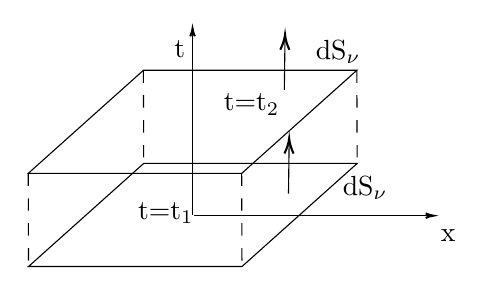
\begin{tikzpicture}[x=0.25pt,y=0.25pt,yscale=-1,xscale=1]
%uncomment if require: \path (0,514); %set diagram left start at 0, and has height of 514

%Straight Lines [id:da944915482116456] 
\draw    (250.32,299.23) -- (250.32,32) ;
\draw [shift={(250.32,30)}, rotate = 90] [color={rgb, 255:red, 0; green, 0; blue, 0 }  ][line width=0.75]    (10.93,-3.29) .. controls (6.95,-1.4) and (3.31,-0.3) .. (0,0) .. controls (3.31,0.3) and (6.95,1.4) .. (10.93,3.29)   ;
%Straight Lines [id:da15966795743012707] 
\draw    (252.32,300.23) -- (596.16,300.23) ;
\draw [shift={(598.16,300.23)}, rotate = 180] [color={rgb, 255:red, 0; green, 0; blue, 0 }  ][line width=0.75]    (10.93,-3.29) .. controls (6.95,-1.4) and (3.31,-0.3) .. (0,0) .. controls (3.31,0.3) and (6.95,1.4) .. (10.93,3.29)   ;
%Shape: Rectangle [id:dp13264483463125742] 
\draw   (179.7,224.73) -- (488.23,224.73) -- (321.76,373.73) -- (13.23,373.73) -- cycle ;
%Shape: Rectangle [id:dp5241947086840221] 
\draw   (179.29,90.11) -- (487.82,90.11) -- (321.35,239.11) -- (12.82,239.11) -- cycle ;
%Straight Lines [id:da9873328008653245] 
\draw    (383,118.5) -- (383.98,40.5) ;
\draw [shift={(384,38.5)}, rotate = 90.72] [color={rgb, 255:red, 0; green, 0; blue, 0 }  ][line width=0.75]    (21.86,-6.58) .. controls (13.9,-2.79) and (6.61,-0.6) .. (0,0) .. controls (6.61,0.6) and (13.9,2.79) .. (21.86,6.58)   ;
%Straight Lines [id:da7100914300813527] 
\draw    (389,268.5) -- (389.98,190.5) ;
\draw [shift={(390,188.5)}, rotate = 90.72] [color={rgb, 255:red, 0; green, 0; blue, 0 }  ][line width=0.75]    (21.86,-6.58) .. controls (13.9,-2.79) and (6.61,-0.6) .. (0,0) .. controls (6.61,0.6) and (13.9,2.79) .. (21.86,6.58)   ;
%Straight Lines [id:da5752286958121103] 
\draw  [dash pattern={on 4.5pt off 4.5pt}]  (12.82,239.11) -- (13.23,373.73) ;
%Straight Lines [id:da3625750970621462] 
\draw  [dash pattern={on 4.5pt off 4.5pt}]  (179.29,90.11) -- (179.7,224.73) ;
%Straight Lines [id:da36524075127919386] 
\draw  [dash pattern={on 4.5pt off 4.5pt}]  (487.82,90.11) -- (488.23,224.73) ;
%Straight Lines [id:da5000478553674463] 
\draw  [dash pattern={on 4.5pt off 4.5pt}]  (321.35,239.11) -- (321.76,373.73) ;

% Text Node
\draw (210,32.51) node [anchor=north west]   [align=left] {{t }};
% Text Node
\draw (595,306.78) node [anchor=north west]   [align=left] {{x}};
% Text Node
\draw (266,267) node [anchor= north east]   [align=left] {{ t=t\textsubscript{1}}};
% Text Node
\draw (268,110) node [anchor=north west]   [align=left] {{ t=t\textsubscript{2}}};
% Text Node
\draw (401,32) node [anchor=north west]   [align=left] {{ dS\textsubscript{$\nu $}}};
% Text Node
\draw (440,260) node [anchor=  west]   [align=left] {{ dS\textsubscript{$\nu $}}};
\end{tikzpicture}
\end{minipage}
\begin{minipage}[t]{0.48\textwidth}
    \vspace*{0pt} 
    This is an integral of the flux along the time direction. \par
    So the expression of $\Delta p^{\mu }_{ \text{ total }}$ can be written as \par
\end{minipage}

\[
= \int_{ \text{ total surface }}^{}{dS_{\nu }T^{\mu \nu }} = \int_{Volume}^{}{dx^{3}\partial_{\nu }T^{\mu \nu }} = \int_{volume}^{}{dV \partial_{\nu }T^{\mu \nu }}
\]
So we have two surfaces and we closed it inside a solid, and it is like we are doing gauss theorem, We can use the divergence theorem in 4d. We state that the divergence of $T^{\mu \nu }$:
\begin{gather*}
\partial_{\mu }T^{\mu \nu } = 0 \\
\partial_{\nu }T^{\mu \nu } = 0
\end{gather*}
And that's a way to express conservation.

\paragraph{Results for perfect fluids}
\[
T^{\mu \nu } = \left( \rho  +p \right) u^{\mu }u^{\nu }+p \eta^{\mu \nu }
\]
and taking the derivative
\begin{gather*}
\partial_{\mu } T^{\mu \nu } = \partial_{\mu }\left( \rho +p \right)u^{\mu }u^{\nu } + \partial_{\mu }p \eta^{\mu \nu } + \left( \rho +p \right)\left( \partial_{\mu }u^{\mu } \right)u^{\nu } + \left( \rho +p \right) u^{\mu }\partial_{\mu }u^{\nu } = \\
= \partial_{\mu }\left( \rho +p \right)u^{\mu }u^{\nu }+ \partial_{\mu }p \eta^{\mu \nu } + \left( \rho +p \right) [\left( \partial_{\mu }u^{\mu }u^{\nu } + u^{\mu }\partial_{\mu }u^{\nu } \right)]
\end{gather*}
It is quite clear, just the thing that we neglect derivative of the metric because in flat spacetime it is a constant matrix, and so it's 0.\par
Let's take the projection of this identity along the direction of the four-velocity.
\begin{gather*}
	u_{\nu }\partial_{\mu }T^{\mu \nu } = -\partial_{\mu }\left( \rho +p \right)u^{\mu }+\left( \partial_{\mu }p \right)u^{\mu }+\left( \rho +p \right)[-\partial_{\mu }u^{\mu }+u_{\nu }u^{\mu }\partial_{\mu }u^{\nu }] =
\end{gather*}
and since, 
\[
\partial_{\mu }\left( u_{\nu }u^{\nu } \right) = 0 = \partial_{\mu }\left( -1 \right)
\]
we get
\begin{equation}
= -\partial_{\mu }\left( \rho +p \right)u^{\mu } + \partial_{\mu }p u^{\mu }- \left( \rho +p \right)\partial_{\mu }u^{\mu } = 0
\end{equation}
And in the NR limit, $p\ll \rho $:
\begin{gather*}
-\partial_{\mu }\rho  u^{\mu }+\rho \partial_{\mu }u^{\mu }+ \partial_{\mu }pu^{\mu }=0 \\
\text{ we can neglect the last term since the hypothesis } \\
\partial_{\mu }\left( \rho u^{\mu } \right) = 0 \implies \partial_{t}\rho +\partial_{i}\left( \rho u^{i} \right) = 0
\end{gather*}
we recover the continuity equation.

\paragraph{exercise}: instead of projecting on $u^{\nu  }$, project orthogonal to $u^{\mu }$,compute: $p^{\alpha }_{\nu } \partial_{\mu }T^{\mu \nu }=0$.
idk what it means: $p^{\alpha }_{\beta }\equiv \delta^{\alpha }_{\beta } + u^{\alpha }u_{\beta }$. Evaluate alpha = 1,2,3.






\section{Lec 7}

\subsection{Equivalence Principle}

The idea of the \emph{universality} of the gravitational interaction, in the form of the \emph{Equivalence principle } led Einstein to think that gravity is special, not just another field, but a metric tensor that describes the curvature of spacetime.

\subsubsection{Weak Equivalence Principle, WEP}
It states that \emph{inertial} mass and \emph{gravitational} mass of any object are equal. \par
From the Second Law of Mechanics:
\[
 \vec{F}= m_{i}\vec{a}
\]
with $m_{i}=$ inertial mass.
While to quantify gravitational forces in Newtonian mechanics:
\[
\vec{F} = -m_{g} \nabla \Phi_{g}
\]
With $\nabla \Phi_{g}$ gradient of scalar field $\Phi_{g}$, known as gravitational potential.
From these formulas, we see no actual reason why $m_{i} = m_{g}$:
\begin{itemize}
	\item The inertial mass has a universal character, it takes the same value no matter what kind of force is being exerted.
	\item The gravitational mass is a quantity specific to the gravitational force. One could think $ \frac{m_{g}}{m_{i}}$ as the \emph{gravitational charge}.
\end{itemize}
Galileo showed by rolling balls down the inclined plane, that the response of matter to gravitation is universal, and in Newtonian mechanics it translates in WEP:
\[
m_{i }= m_{g}
\]
This, for freely falling objects, becomes
\[
a = -\nabla \Phi 
\]

This led to think an equivalent formulation of WEP that is: \emph{there exists a preferred class of trajectories through space time, called Inertial or Freely-Falling}.
Freely falling is intended as "moving under the sole influence of gravity", these objects are unaccelerated. \par

The universality of gravitation can be stated in another form:
\indent If we consider a physicist in a spaceship that is accelerating at a constant rate, like
\[
\vec{a} = - \vec{g}
\]
he would be not able to distinguish by scientific experiments the situation in which he sits on Earth's surface. (Restricted to local observation).


\tikzset{every picture/.style={line width=0.75pt}} %set default line width to 0.75pt

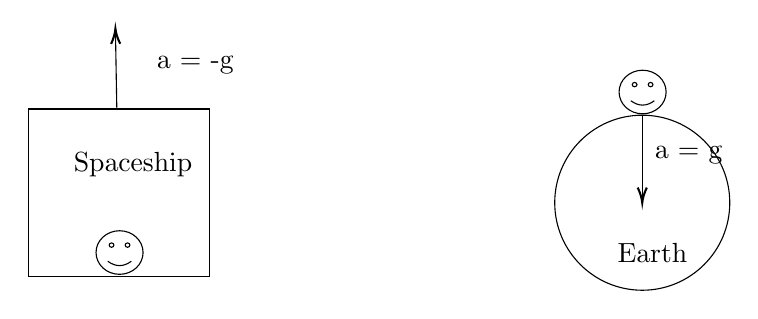
\begin{tikzpicture}[x=0.5pt,y=0.5pt,yscale=-1,xscale=1]
%uncomment if require: \path (0,300); %set diagram left start at 0, and has height of 300

%Shape: Rectangle [id:dp8176008658551641]
\draw   (98,85.5) -- (229,85.5) -- (229,206.5) -- (98,206.5) -- cycle ;
%Shape: Circle [id:dp5519338819044518]
\draw   (478.5,153.25) .. controls (478.5,118.32) and (506.82,90) .. (541.75,90) .. controls (576.68,90) and (605,118.32) .. (605,153.25) .. controls (605,188.18) and (576.68,216.5) .. (541.75,216.5) .. controls (506.82,216.5) and (478.5,188.18) .. (478.5,153.25) -- cycle ;
%Shape: Smiley Face [id:dp2317824195662611]
\draw   (147,189.25) .. controls (147,180.55) and (154.61,173.5) .. (164,173.5) .. controls (173.39,173.5) and (181,180.55) .. (181,189.25) .. controls (181,197.95) and (173.39,205) .. (164,205) .. controls (154.61,205) and (147,197.95) .. (147,189.25) -- cycle ; \draw   (156.52,183.9) .. controls (156.52,183.03) and (157.28,182.32) .. (158.22,182.32) .. controls (159.16,182.32) and (159.92,183.03) .. (159.92,183.9) .. controls (159.92,184.76) and (159.16,185.47) .. (158.22,185.47) .. controls (157.28,185.47) and (156.52,184.76) .. (156.52,183.9) -- cycle ; \draw   (168.08,183.9) .. controls (168.08,183.03) and (168.84,182.32) .. (169.78,182.32) .. controls (170.72,182.32) and (171.48,183.03) .. (171.48,183.9) .. controls (171.48,184.76) and (170.72,185.47) .. (169.78,185.47) .. controls (168.84,185.47) and (168.08,184.76) .. (168.08,183.9) -- cycle ; \draw   (155.5,195.55) .. controls (161.17,199.75) and (166.83,199.75) .. (172.5,195.55) ;
%Shape: Smiley Face [id:dp04372115955443423]
\draw   (525,73.25) .. controls (525,64.55) and (532.61,57.5) .. (542,57.5) .. controls (551.39,57.5) and (559,64.55) .. (559,73.25) .. controls (559,81.95) and (551.39,89) .. (542,89) .. controls (532.61,89) and (525,81.95) .. (525,73.25) -- cycle ; \draw   (534.52,67.9) .. controls (534.52,67.03) and (535.28,66.32) .. (536.22,66.32) .. controls (537.16,66.32) and (537.92,67.03) .. (537.92,67.9) .. controls (537.92,68.76) and (537.16,69.47) .. (536.22,69.47) .. controls (535.28,69.47) and (534.52,68.76) .. (534.52,67.9) -- cycle ; \draw   (546.08,67.9) .. controls (546.08,67.03) and (546.84,66.32) .. (547.78,66.32) .. controls (548.72,66.32) and (549.48,67.03) .. (549.48,67.9) .. controls (549.48,68.76) and (548.72,69.47) .. (547.78,69.47) .. controls (546.84,69.47) and (546.08,68.76) .. (546.08,67.9) -- cycle ; \draw   (533.5,79.55) .. controls (539.17,83.75) and (544.83,83.75) .. (550.5,79.55) ;
%Straight Lines [id:da28786648084951405]
\draw    (162,84.5) -- (161.04,29.5) ;
\draw [shift={(161,27.5)}, rotate = 88.99] [color={rgb, 255:red, 0; green, 0; blue, 0 }  ][line width=0.75]    (10.93,-3.29) .. controls (6.95,-1.4) and (3.31,-0.3) .. (0,0) .. controls (3.31,0.3) and (6.95,1.4) .. (10.93,3.29)   ;
%Straight Lines [id:da9125944015659164]
\draw    (541.75,90) -- (541.75,151.25) ;
\draw [shift={(541.75,153.25)}, rotate = 270] [color={rgb, 255:red, 0; green, 0; blue, 0 }  ][line width=0.75]    (10.93,-3.29) .. controls (6.95,-1.4) and (3.31,-0.3) .. (0,0) .. controls (3.31,0.3) and (6.95,1.4) .. (10.93,3.29)   ;

% Text Node
\draw (189,46) node [anchor=north west][inner sep=0.75pt]   [align=left] {a = -g};
% Text Node
\draw (549,111) node [anchor=north west][inner sep=0.75pt]   [align=left] {a = g};
% Text Node
\draw (522,181) node [anchor=north west][inner sep=0.75pt]   [align=left] {Earth};
% Text Node
\draw (129,115) node [anchor=north west][inner sep=0.75pt]   [align=left] {Spaceship};


\end{tikzpicture}
\bigskip\hfill

If the spaceship would be sufficiently big, we would see that the effect of acceleration would always be in the same direction, while on the surface or the Earth we would see that it points towards the center of the earth, so radial vs straight parallel lines.\par
So WEP could be stated as \emph{the motion of freely-falling particles are the same in a gravitational field and a uniformly accelerated frame, in small enough regions of spacetime}. In larger regions there would be inhomogenities, which will lead to tidal forces.

\subsubsection{Einstein's Equivalence Principle, EEP}
The Einstein Equivalence Principle is just a little generalization of the WEP:
\begin{quote}
In small enough regions of spacetime, the laws of physics reduce to those of special relativity: it is impossible to detect the existence of gravitational field by means of local experiments.
\end{quote}
Consider a hydrogen atom, a bound state of a proton and an electron. Its mass
is actually less than the sum of the masses of the proton and electron considered
individually, because there is a negative binding energy—you have to put energy
into the atom to separate the proton and electron. According to the WEP, the  gravitational mass of the hydrogen atom is therefore less than the sum of the masses of its constituents; the gravitational field couples to electromagnetism (which holds the atom together) in exactly the right way to make the gravitational mass come out right. This means that not only must gravity couple to rest mass universally, but also to all forms of energy and momentum—which is practically the claim of the EEP.

It is the EEP that implies that we should attribute the action of gravity the curvature of spacetime.

\subsubsection{Strong Equivalence Principle, SEP}
Is defined to include all of the laws of physics, gravitational and otherwise.
We will define \emph{unaccelerated} as \emph{freely falling}, from here we decide that gravity is not a force, because a force leads to acceleration, and our definition of zero acceleration is \emph{ moving freely in the presence of whatever gravitational field happens to be around.} \par

We know that there is a class of preferred frames: Inertial Frames (where laws of dynamics are true).
We introduce a new class of frames: Freely Falling Frames, where \emph{ unaccelerated particles move only due to gravity.} \par
Obviously these frames must be local frames, otherwise, due to inhomogenities on the gravitational field, particles initially at rest will begin to move with respect to such frame.
\begin{figure}[h]
\centering
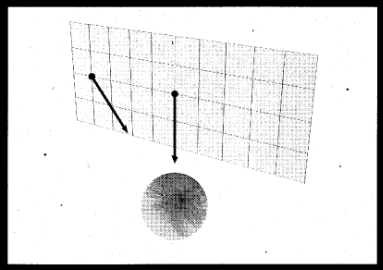
\includegraphics[width=0.8\linewidth]{imm/failureglobal.png}
\caption{The failure of global frames.}
\label{imm:failureglobal}
\end{figure}

After this we need a mathematical framework were what just said is consistent. The solution is to think that spacetime has a curved geometry and gravitation the manifestation of this curvature.
Before jumping in what is a manifold, let's see if the consequences are of our world.

\subsubsection{Gravitational Redshift}
\begin{figure}[h]
\centering
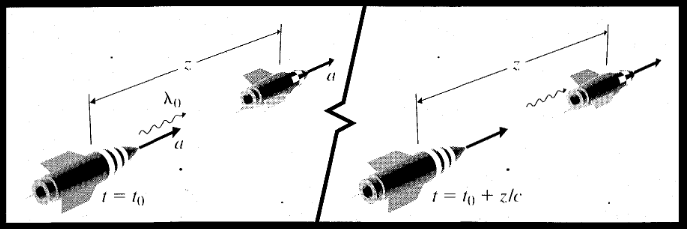
\includegraphics[width=0.8\linewidth]{imm/gravshift1.png}
\caption{Doppler shift measured by two rockets, each feeling acceleration \textbf{a}.}
\label{imm:gravshift1.png}
\end{figure}

Be two spaceships, separated by distance \emph{z}, each moving with constant $\vec{a}$ acceleration in a region without gravitational fields. \par
At \emph{t\textsubscript{0}} ship in the back emits a photos of $\lambda_{0}$.\par
The distance \emph{z} stays constant, so the photon is received after $\Delta t = z/c$ in our reference frame. At $t = t_{0}+ \Delta t$ the boxes have picked up an additional velocity $\Delta v = \vec{a}\Delta t = \vec{a}z/c$. The photon reaching the front spaceship will be redshifted bu the Doppler Effect, by \[
\frac{\Delta \lambda }{\lambda_{0}} = \frac{\Delta v}{c} = \frac{a z}{c^{2}}
\]
And according to EEP this should happen also in a uniform gravitational field.\par
\begin{figure}[h]
\centering
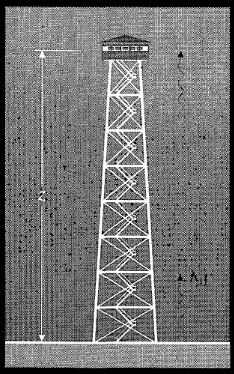
\includegraphics[width=0.3\linewidth]{imm/gravshift2.png}
\caption{Gravitational redshift on Earth's surface}
\label{imm:gravshift2}
\end{figure}
So i a photon e mitted from the ground with $\lambda_{0}$ will be redshifted by
\[
\frac{\Delta  \lambda }{\lambda_{0}} = \frac{a_{g}z}{c^{2}}
\]
To note that is a direct consequence of EEP, no details of GR were required.
The thing is, if i try to represent this with Minkowski metric, I don't notice the redshift.

So now we really need to talk about Manifolds
\subsection{Manifolds}
A manifold is a space that may be curved and have a complicated topology, but in local regions looks just like $\mathbb{R}^{n}$. A crucial part is that the dimensionality \emph{n} of the Euclidean Spaces being used must be the same in every patch of the manifold.
For example are not manifolds, a line ending on a plane and two cones intersecting at their vertices.\par
\begin{figure}[h]
\centering
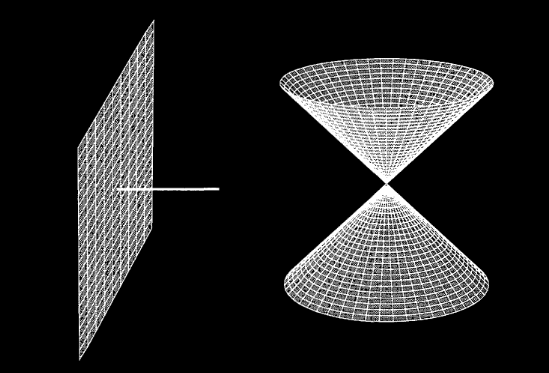
\includegraphics[width=0.5\linewidth]{imm/notmanifold.png}
\caption{Not manifolds}
\label{imm:notmanifold.png}
\end{figure}

\subsubsection{Coordinate System}
Be 
\begin{equation}
\begin{cases}
U\subset M \\
\phi : U \to \mathbb{R}^{n} \\
\phi\left( U \right) \text{ is open in }\mathbb{R}^{n}
\end{cases}
\end{equation}
These are a system of conditions to define a coordinate system or \emph{chart.}\par
\begin{figure}[h]
\centering
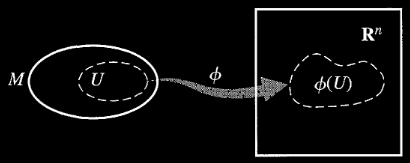
\includegraphics[width=0.65\linewidth]{imm/chart.png}
\caption{A coordinate chart covering an open subset \emph{U} of \emph{M}.}
\label{imm:chart}
\end{figure}
An \emph{atlas} is a indexed collection of charts $\{\left( U_{\alpha}, \phi_{\alpha } \right)\}$.

\subsubsection{Vectors again}
One point we stressed was the notion of a tangent space, the set of all vectors at a single point in spacetime. A vector is not a thing that stretches from one point to another but is an object associated with a single point. \par
Be $f : M \to \mathbb{R}$. Each curve passing through a point \emph{P}, defines an operator, the \emph{ directional derivative}, which maps $f \to df/d\lambda \left( \text{ at }p \right)$. \par
We claim the tangent space $T_{P}$ can be identified with the space of directional derivative operators along curves through \emph{P}.
And for any \emph{f} we can write:
\[
\frac{df}{d\lambda } = \frac{df}{dx^{\mu }} \frac{dx^{\mu }}{d\lambda } \implies \frac{d}{d\lambda } = \frac{dx^{\mu }}{d\lambda } \partial_{\mu }
\]
If i change the coordinates i can apply the chain rule.

\section{Lec 8}
\subsection{Brief Recap}
We saw the WEP, that states $m_{i}= m_{g}$, and as consequence we get that is is impossible distinguish a gravitational field from motion, at least locally. \par
With the EEP we were able to derive the expression that quantify the gravitational redshift.
The SEP included gravity.\par

Focusing on EEP, we introduced \emph{Locally Inertial Frames, LIF} (equivalent to Freely Falling Frames).
Having accepted that gravity cannot be treated as a force, because it is impossible to disentangle acceleration due to gravity, we identified a preferred class of frames: LIFs.\par
In LIFs laws of physics are equal to the laws of SR and spacetime is\break Minkowskian.

We introduced Coordinates: with a generic set M, a chart, given a subset $U \subset M $, is a injective linear  map $\phi $, that \[
\phi : U \to \mathbb{R}^{n}
\]
An \emph{atlas }is an indexed $\{U_{\alpha}, \phi_{\alpha }\}$, in such a way that $U_{\alpha }$ cover \emph{M}.
A \emph{manifold} is a set M along with an atlas. A manifold can be $C^{\infty}$ if $\phi $ are differentiable an infinite amount of times, otherwise is $C^{p}$, differentiable p-times.
\subsubsection{Vectors again and again}
We resurrected $T_{P}$, \emph{P} generic \emph{M} point. $T_{P}$ is the vector space of all the vectors defined at that point.
\begin{quote}
$T_{P}$ is identified with the space of directional derivatives operators acting along the curves through \emph{P}
\end{quote}
Why this identification makes sense?\par
A generic curve through spacetime, that we call WL, is a parametric curve that is indicated by $x^{\mu }\left( \lambda  \right)$: for a specific value of $\lambda $ I have the $x^{\mu }$ point.
\[
x^{\mu }\left( \overline{\lambda } \right) = P
\]
How do I define the directional derivatives?
Be \[
\frac{d}{d\lambda }
\]
that acts on functions, \emph{f},
\[
f : M \to \mathbb{R}
\]
then $\forall f$:
\[
\frac{d}{d\lambda } = \frac{dx^{\mu }}{d\lambda }\partial_{\mu }
\]
We see that it is like a basis.\par
\textbf{Basis vectors } for $T_{P}\to \partial_{\mu }$. (we previously called them $\hat{e}_{\left( \mu  \right)}$). \par
In conclusion a generic vector is 
\[
V = V^{\mu }\partial_{\mu }
\]
where $V^{\mu }$ are the components, and $\partial_{\mu }$ are the basis elements.\par

It's very easy to show how vectors transform because we know how derivatives transform:
\begin{equation}
\frac{\partial}{\partial  x^{\mu'}} = \frac{\partial  x^{\mu }}{\partial  x^{\mu '}} \frac{\partial}{\partial  x^{\mu }}
\end{equation}
or in a tensor-like notation:
\begin{equation}
\partial_{\mu '} = \frac{\partial  x^{\mu }}{\partial x^{\mu '}} \partial_{\mu }
\end{equation}
If \emph{V} tensor is invariant, by definition, it's components transform anyway like
\[
V^{\mu '} = \frac{\partial x^{\mu '}}{\partial x^{\mu }}V^{\mu }
\]

\paragraph{Example} LTs
\[
x^{\alpha '} = \Lambda^{\alpha '}_{\alpha }x^{\alpha }
\]
I consider a specific change of coordinates: LTs, so
\[
\frac{\partial x^{\mu '}}{\partial x^{\mu }} = \frac{\partial}{\partial x^{\mu }} \left( \Lambda^{\mu '}_{\alpha }x^{\alpha } \right) = \Lambda^{\mu '}_{\alpha } \frac{\partial x^{\alpha }}{\partial x^{\mu }} = \Lambda^{\mu '}_{\alpha } \delta^{\alpha }_{\mu } = \Lambda^{\mu '}_{\mu }
\]
we get under more general transformations vectors components transform like this, and more, we recovered the LT transformation.

\subsection{Dual Vectors}
Be the \emph{cotangent space} $T_{P}^{*}$. If $\omega \in T_{P}^{*}$, $\omega$ is a linear map that  $\omega : T_{P}\to \mathbb{R}$.
We want to define formally $T_{P}^{*}$ (like we did for $T_{P}$).
We know that the tangent space $T_{P}$ holds directional derivatives, while cotangent space $T_{P}^{*}$ holds gradients. \par
For a generic $f: M\to \mathbb{R}$:
\begin{gather*}
\frac{d}{d\lambda } \in T_{P} \\
d \in T_{P}^{*} \\
\text{ and so } \\
df \left( \frac{d}{d\lambda } \right) \equiv \frac{df}{d\lambda }\\
\downarrow \quad\; \downarrow \qquad \;\downarrow \\
\in T_{P}^{*}, \in T_{P}, \in \mathbb{R}
\end{gather*}
\textbf{Basis} for T\textsubscript{P}\textsuperscript{*}: $dx^{\mu }$.\par
\[
dx^{\mu } \left( \frac{\partial}{\partial x^{\nu }} \right) = \frac{\partial x^{\mu }}{\partial x^{\nu }} = \delta^{\mu }_{\nu }
\]
that is the same as the old $\hat{O}^{\left( \mu  \right)}\left( \hat{e}_{\nu } \right)=\delta^{\mu }_{\nu }$.

A dual vector is \[
\omega = \omega_{\mu }dx^{\mu }
\]
the basis component transform like
\[
dx^{\mu '} = \frac{\partial x^{\mu '}}{\partial x^{\mu }} dx^{\mu }
\]
and the vector components
\[
\omega_{\mu '} = \frac{\partial x^{\mu }}{\partial x^{\mu '}}\omega_{\mu }
\]

\subsection{Tensors (k,l)}
\[
T : T_{P}^{*}\times \ldots \times T_{P}^{*} \times T_{P}\times \ldots \times T_{P}\to \mathbb{R}
\]
Tensors can be expanded into components:
\[
T = T^{\mu_{1}\ldots \mu_{k}}_{\nu_{1}\ldots \nu_{l}} \left( \partial_{\mu_{1}} \otimes \ldots \otimes \partial_{\mu_{k}} \otimes dx^{\nu_{1}} \otimes \ldots \otimes dx^{\nu_{l}} \right)
\]
So the components of a generic tensor transform like
\[
T^{\mu_{1}' \ldots \mu_{k}'}_{\nu_{1}' \ldots \nu_{l}'} = \left( \frac{\partial x^{\mu_{1}'}}{\partial x^{\mu_{1}}} \ldots \frac{\partial x^{\nu_{1}}}{\partial x^{\nu_{1}'}}\ldots  \right) T^{\mu_{1}\ldots \mu_{k}}_{\nu_{1}\ldots \nu_{l}}
\]

Now let's see a unusual tensor, it's a (2,1) tensor, how does transform?
\[
T^{\alpha' \beta'}_{\gamma'} = \frac{\partial x^{\alpha '}}{\partial x^{\alpha }} \frac{\partial x^{\beta '}}{\partial x^{\beta }} \frac{\partial x^{\gamma }}{\partial x^{\gamma '}} T^{\alpha \beta }_{\gamma }	 
\]
\paragraph{Example/exercise} (from 2.4 of Carroll)
Be a tensor $S_{ij}$, with $i,j =1,2$, so it's a (0,2) tensor.
We know that
\begin{itemize}
	\item S\textsubscript{11} = 1
	\item S\textsubscript{12}=S\textsubscript{21} = 0
	\item S\textsubscript{22} = x\textsuperscript{2}
\end{itemize}
We get new coordinates:
\begin{gather*}
x' = \frac{2x}{y} \\
y' = \frac{y}{2}
\end{gather*}
What are the expressions for $S_{i'j'}$?\par
One could think to compute each entry doing
\[
S_{i'j'}= \frac{\partial x^{i}}{\partial x^{i'}} \frac{\partial x^{j}}{\partial x^{j'}} S_{ij}
\]
So, like the (1,1) one looks like
\[
S_{1'1'} = \frac{\partial x^{i}}{\partial x^{1'}} \frac{\partial x^{j}}{\partial x^{1'}} S_{ij}
\]
It is good exercise to do this. (see sec \ref{ex:changebasis})
But it seems that there is a much faster way than this.\par
We can write the tensor $S$ as
\[
S = S_{\mu \nu }\left( dx^{\mu } \otimes dx^{\nu } \right)
\]
and for our case 
\[
S = S_{ij}\left( dx^{i} \otimes dx^{j} \right)
\]
The action of this tensor could be written as 
\begin{equation}\label{eq:1}
S \left( dx^{i},dx^{j} \right) = S_{11}dx^{2} + S_{12}dxdy + S_{21}dydx + S_{22}dy^{2} = dx^{2} +x^{2}dy^{2}		
\end{equation}
the two middle terms are not grouped because tensor product does not commute.\par

Now we can take the inverse coordinate transformation and write it down.
\begin{equation}
\begin{cases}
x = x'y' \\
 y = 2y'\\
\end{cases} \to 
\begin{cases}
dx = x'dy' + y'dx' \\
dy = 2dy' \\
\end{cases}
\end{equation}
and then we substitute inside eq. [\ref{eq:1}], getting
\begin{gather*}
	\left( x'dy' + y'dx' \right)^{2} + 4dy'^{2} = \\
	x'^{2}dy'^{2} + y'^{2}dx'^{2} + x'y'\left( dx'dy'+dy'dx' \right) + 4dy'^{2} 
\end{gather*}
so we get:
\begin{equation}
\begin{cases}
S_{ii} = y'^{2} \\
S_{ij} = S_{ji} = x'y' \\
S_{jj} = x'^{2} + 4\left( x'y' \right)^{2}
\end{cases}
\to 
\begin{pmatrix}
y'^{2} & x'y' \\
x'y' & x'^{2}+4\left( x'y' \right)^{2}
\end{pmatrix} = S_{i'j'} 
\end{equation}

\subsection{Special Tensors}
Special tensor that we will see are
\begin{itemize}
	\item Derivative
	\item Metric tensor
	\item Levi-Civita Symbol
\end{itemize}

\subsubsection{Derivative}
We will show that the derivative of a tensor is not a tensor anymore.\par

Derivative of a scalar is a (0,1) tensor.
\[
\partial_{\mu }\phi \to \partial_{\mu '}\phi = \frac{\partial x^{\mu }}{\partial x^{\mu '}} \partial_{\mu }\phi 
\]
$\phi $ does not change under transformation, but the derivative does.

Derivative of a tensor $\neq$ tensor:\par
\textbf{example} : 
\[
A_{\mu \nu } = \partial_{\mu }V_{\nu }
\]
But why? \par
Let's transform it:
\begin{gather*}
A_{\mu '\nu '} = \partial_{\mu '}V_{\nu '} = \frac{\partial x^{\mu }}{\partial x^{\mu '}} \frac{\partial }{\partial x^{\mu }} \left( \frac{\partial x^{\nu }}{\partial x^{\nu '}}V_{\nu }  \right) = \\
\text{now if we apply the partial derivative we obtain}\\
= \frac{\partial x^{\mu }}{\partial x^{\mu '}} \frac{\partial x^{\nu }}{\partial x^{\nu '}} \partial_{\mu } V_{\nu } + \left( \frac{\partial x^{\mu }}{\partial x^{\mu '}}  \right)\left( \frac{\partial^{2}x^{\nu }}{\partial x^{\nu '}\partial x^{\mu }}  \right)V_{\nu }
\end{gather*}
What happened? We see there is a piece that we don't like. This second piece is 0 for LTs, because they are linear so second derivatives are null. This because in Euclidean space the derivative is independent on the coordinates, and on Minkowski space too, since it's flat. \par
The tensor itself is independent of the coordinate system, but the operation of taking a partial derivative is highly dependent on what coordinate system you're using.\par
We give importance to this anyway because GR is not a theory for just LTs.
We will develop a covariant derivative that applied to a tensor will give back a tensor.

\subsubsection{Metric tensor}
The roles of the metric tensor are many:
\begin{itemize}
	\item supplies a notion of \emph{past} and \emph{future}
	\item allows the computation of path length and proper time
	\item determines the \emph{shortest distance} between two points
	\item replaces the Newtonian gravitational field $\phi $
	\item provides a notion of locally inertial frames
	\item determines causality
	\item replaces the Euclidean 3D dot product of Newtonian mechanics.
\end{itemize}

We know the Minkowski's one:
\begin{equation}
\eta_{\mu \nu } = \text{diag }\left( -1,1,1,1 \right) = \begin{pmatrix}
-1 & 0 & 0 & 0 \\
0 & 1 & 0 & 0 \\
0 & 0 & 1 & 0 \\
0 & 0 & 0 & 1
\end{pmatrix} 
\end{equation}
\bigskip
In general $g_{\mu \nu }$ will be the metric tensor.\par
We assume the determinant of $g_{\mu \nu }: \text{det}\left( g_{\mu \nu } \right) \equiv g \neq 0 \to $ the metric tensor is \emph{invertible}.
\[
g_{\mu \nu }g^{\nu \alpha } = \delta^{\alpha }_{\mu } \text{ ; } g^{\mu \nu }g_{\nu \alpha } = \delta^{\mu }_{\alpha }
\]
A constant metric tensor implies not curvature.\par
A metric tensor that depends explicitly on the coordinates must describe a non-flat space? \textbf{FALSE} e.g. the polar coordinates: writing $\eta_{\mu \nu }$ in them
\begin{equation}
\eta_{\mu \nu }^{\left(polar\right)} = \begin{pmatrix}
-1 & 0 & 0 & 0 \\
0 & 1 & 0 & 0 \\
0 & 0 & r^{2} & 0 \\
0 & 0 & 0 & r^{2} \text{sin}^{2}\theta ,
\end{pmatrix} 
\end{equation}.
Given a generic metric $g_{\mu \nu }$ and a given event P, it is always possible to find new coordinates:
\[
g_{\hat{\mu }\hat{\nu }} = \frac{\partial x^{\mu }}{\partial x^{\hat{\mu }}} \frac{\partial x^{\nu }}{\partial x^{\hat{\nu }}} g_{\mu \nu }
\]
And
\[
g_{\hat{\mu }\hat{\nu }}\left( P \right) = \eta_{\hat{\mu }\hat{\nu }} \text{ ; } \partial_{\hat{\sigma }}g_{\hat{\mu }\hat{\nu }}\left( P \right)=0
\]
This recalls the definition of LIFs.


\subsection{Applying tensor transformation formula}\label{ex:changebasis}

This is the suggested-to-try alternative way to do the exercise about tensor change of basis. I did it, and since I'm not that good with tensors I thought it is not trivial so will report here.\par
\[
S_{i\prime j\prime } = \frac{\partial x^{i}}{\partial x^{i\prime }} \frac{\partial x^{j}}{\partial x^{j\prime }} S_{ij}
\]
Partial derivatives are a jacobian. So one need to express \emph{x,y} in terms of $x^{\prime },y^{\prime }$, and then derive them to fill the jacobian
\begin{equation}
\frac{\partial x^{i}}{\partial x^{i\prime }}  = \begin{pmatrix}
\partial x /\partial x^{\prime } & \partial x / \partial y^{\prime } \\
\partial y / \partial x^{\prime } & \partial y / \partial y^{\prime }
\end{pmatrix} 
\end{equation}
Express $S_{ij}$ in terms of $x^{\prime }, y^{\prime }$:
\[
S_{ij} = \begin{pmatrix}
1 & 0 \\
0 & \left( x^{\prime }y^{\prime } \right)^{2}
\end{pmatrix} 
\]
And then compute each entry
\[
S_{1^{\prime }1^{\prime }} = \frac{\partial x^{i}}{\partial x^{1\prime }} \frac{\partial x^{j}}{\partial x^{1\prime }} S_{ij} 
\]
et cetera. 



\section{Lec 9}
\subsubsection{Active and passive transformations}
Active transformations change the physical position of a set of points relative to a fixed coordinate system. \par
Passive transformations leave the points fixed but change the coordinate system relative to which they are described.
We prefer the first approach, we leave vectors untouched and transform RFs.

\subsection{Still on Metric Tensor}
We described a little this tensor in the previous lecture. I remember that:
\[
det\left( g \right) = g \neq 0
\]
in 3D Euclidean Space
\[
	g = \mathbb{I} = \begin{pmatrix}
	1 & 0 & 0 \\
	0 & 1 & 0 \\
	0 & 0 & 1
	\end{pmatrix} 		
\]
and in spherical it would be like
\[
\begin{pmatrix}
1 & 0 & 0 \\
0 & r^{2}sin^{2}\theta  & 0 \\
0 & 0 & r^{2}
\end{pmatrix} 
\]
In general the metric tensor has this form
\[
g_{\mu \nu } = diag\left( -1, \ldots, 1, \ldots , 0, \ldots   \right)
\]
If there are just '$+1$', the metric is Euclidean.\par
If I have one ' $-1$' and only ' $+1$' the metric is Lorentzian.\par
We will not discuss other combinations.

Today we will try to formalize EEP.\par

Let $P$ be a spacetime point and 
\[
g_{\mu \nu }\left( P \right)= \text{ some generic matrix } \neq \eta_{\mu \nu }
\]
I want to find new coordinates $x^{\hat{\mu }}$ such that $g_{\hat{\mu }\hat{\nu }}\left( P \right)=\eta_{\mu \nu }$ and $\partial_{\hat{\rho }}g_{\hat{\mu }\hat{\nu }}\left( P \right)=0$.
If you watch the last expression you see that it includes 40 different expressions $\left( 64/2 \right)+8$

I choose $x^{\mu }_{P}= x^{\hat{\mu }}_{P}=0$, so $P$ is the origin of both frames. So I get
\[
g_{\hat{\mu }\hat{\nu }}\left( x^{\hat{\alpha }} \right) = \frac{\partial x^{\mu }}{\partial x^{\hat{\mu }}} \frac{\partial x^{\nu }}{\partial x^{\hat{\nu }}} g_{\mu \nu }\left( x^{\alpha } \right) 
\]
I'm interested in transformations around $P$, so I see that spacetime is locally Minkoskian.\par
Doing a Taylor expansion I will see that first order is Minkoskian:
\begin{equation}
x^{\mu }\left( x^{\hat{\mu }} \right) = \left( \frac{\partial x^{\mu }}{\partial x^{\hat{\mu }}}  \right)_{P}x^{\hat{\mu }} + \frac{1}{2}\left( \frac{\partial^{2}x^{\mu }}{\partial x^{\hat{\mu }}\partial  x^{\hat{\nu }}}  \right)_{P}x^{\hat{\mu }}x^{\hat{\nu }}+ \frac{1}{6} \left( \frac{\partial^{3}x^{\mu }}{\partial x^{\hat{\mu }}\partial x^{\hat{\nu }}\partial x^{\hat{\rho }} }  \right)_{P} x^{\hat{\mu }}x^{\hat{\nu }}x^{\hat{\rho }}+ \ldots 
\end{equation}

Why did he stop at $3^{rd}$ order? Listen to recording at $\sim 39:00$.
\begin{equation}
\frac{\partial x^{\mu }}{\partial x^{\hat{\mu }}} = \left( \frac{\partial x^{\mu }}{\partial x^{\hat{\mu }}}  \right)_{P} + \left( \frac{\partial^{2}x^{\mu }}{\partial x^{\hat{\mu }}\partial x^{\hat{\alpha }} }  \right)_{P} x^{\hat{\alpha }} +\frac{1}{2} \left( \frac{\partial^{3}x^{\mu }}{\partial x^{\hat{\mu }}\partial x^{\hat{\alpha }} \partial x^{\hat{\beta  }}}  \right)_{P} x^{\hat{\alpha }}x^{\hat{\beta }}
\end{equation}

\begin{equation}
g_{\mu \nu } \left( x^{\alpha } \right) = \left( g_{\mu \nu } \right)_{P} + \left( \partial_{\rho }g_{\mu \nu } \right)_{P} x^{\rho } +\frac{1}{2} \left( \partial_{\rho }\partial _{\sigma } g_{\mu \nu } \right)_{P} x^{\rho }x^{\sigma }+ \ldots 
\end{equation}
Now i just need to write down the metric tensor in new coordinates:
\begin{gather*}
\hat{g} + \left( \hat{\partial }\hat{g} \right)_{P}\hat{x} + \left( \hat{\partial }\hat{\partial }\hat{g} \right)_{P}\hat{x}\hat{x}  = \left( \frac{\partial x}{\partial \hat{x}} \frac{\partial x}{\partial \hat{x}} g \right)_{P} + \left( \frac{\partial x}{\partial \hat{x}}  \frac{\partial^{2}x}{\partial \hat{x} \partial \hat{x}} + \frac{\partial x}{\partial \hat{x}} \frac{\partial x}{\partial \hat{x}} \partial g \right)_{P}\hat{x} + \\
+ \left( \frac{\partial x}{\partial \hat{x}} \frac{\partial^{3}x}{\partial \hat{x} \partial \hat{x} \partial \hat{x}} g + \frac{\partial^{2}x}{\partial \hat{x} \partial \hat{x}} \frac{\partial^{2}x}{\partial \hat{x} \partial \hat{x}} g + \frac{\partial x}{\partial \hat{x}} \frac{\partial^{2}x}{\partial \hat{x} \partial \hat{x}} \partial \hat{g} + \frac{\partial x}{\partial \hat{x}} \frac{\partial x}{\partial \hat{x}} \hat{\partial }\hat{\partial g}   \right) \hat{\partial }\hat{x}
\end{gather*}

This is the structure (with all indices suppressed) of the Taylor expansion (.rec..) around point $P$. \par
It's true to write:
\[
	\hat{g} = A+ B \hat{x} + C \hat{x}\hat{x} + \ldots 
\]
with \emph{A,B,C} the three terms up there. So we can set terms of equal order in $\hat{x}$ on each side equal to each other. Therefore it's like having
\[
	\left( g_{\hat{\mu }\hat{\nu }} \right)_{P} = A = \left( \frac{\partial x}{\partial } \hat{x} \frac{\partial x}{\partial \hat{x}} g  \right)_{P}
\]
On the left we have 10 numbers in all to describe a symmetric two-index tensor, and they are determined by the matrix on the right, This is a $4\times 4$ matrix without constraints, so we have enough freedom to put the 10 numbers of the left tensor into \emph{canonical form}.\par
At first order we have, on the left, four derivatives of 10 components for a total of 40 numbers, while on the right side we have 10 choices of $\hat{\mu }$s and four choices of $\mu$s, for a total of 40 degrees of freedom. This is precisely the number of choices we need to determine all of the first derivatives of the metric, which we can therefore set to 0. \par
At second order with left side the item is symmetric on it's indices in pairs for a total of $10 \times 10 = 100$ numbers, On the right-hand side we have symmetry in the three lower indices gaining 20 possibilities multiplied by four for the upper index we have 80 degrees of freedom, 20 fewer than we require to set the second derivative of the metric to 0.\par

\subsection{Levi Civita symbol}
We like tensors but sometimes we also like nontensorial objects.
Let's remember the Levi Civita symbol 
\[
	\tilde{\epsilon}_{\mu _{1}\ldots \mu _{n }} = \begin{cases}
	+1 \text{ if even permutations } \\
	-1 \text{ if odd permutations } \\
	0 \text{ otherwise }
	\end{cases}	
\]
By definition this symbol has the components specified above in \emph{any} coordinate system, and it is a symbol and not a tensor because it is defined to not change under coordinate transformations, We are able to treat him like tensor only in inertial coordinates in flat spacetime.

If $\epsilon_{\mu \nu \rho \gamma }$ was a tensor then it should transform like
\begin{equation}
\tilde{\epsilon}_{\mu_{1}' \ldots \mu_{n}'} = \frac{\partial x^{\mu_{1}}}{\partial x^{\mu_{1'}}} \ldots \frac{\partial x^{\mu_{n'}}}{\partial x^{\mu_{n'}}} \tilde{\epsilon}_{\mu_{1}\ldots \mu_{n}}
\end{equation}

but this is \textbf{NOT TRUE}.\par
 

We are able to treat it as a tensor only in inertial coordinates of spacetime since LTs would have left the components invariant anyway.\par
It's behaviour can be related to the determinant of a generic matrix $M$:
\[
\tilde{\epsilon}_{\mu_{1'}\ldots \mu_{n'}} \|M\| = \tilde{\epsilon}_{\mu_{1}\ldots \mu_{n}} M^{\mu_{1}}_{\mu_{1'}} \ldots M^{\mu_{n}}_{\mu_{n'}}.
\]

For example, a $2\times 2$ matrix:\par
$M^{\mu }_{\nu }$ with $\mu ,\nu =1,2$.
\begin{gather}
	\tilde{\epsilon }_{12} \cdot det\left( M \right) = det\left( M \right)= \tilde{\epsilon }_{\mu_{1}\mu_{2}} M^{\mu_{1}}_{1} M^{\mu_{2}}_{2} = \\
	= \tilde{\epsilon }_{12} M^{1}_{1} M^{2}_{2} + \tilde{\epsilon }_{21}M^{2}_{1}M^{1}_{2} = M^{1}_{1}M^{2}_{2} - M^{2}_{1}M^{1}_{2} = ad- bc
\end{gather}\par

Setting $M^{\mu }_{\mu '} = \partial x^{\mu } / \partial x^{\mu '} $, we get
\[
\tilde{\epsilon }_{\mu_{1}' \ldots \mu_{n}'} = \left| \frac{\partial x^{\mu '}}{\partial x^{\mu }} \right| \tilde{\epsilon }_{\mu _{1}\ldots \mu_{n}} \frac{\partial x^{\mu _{1}}}{\partial x^{\mu _{1}'}} \ldots \frac{\partial x^{\mu _{n}}}{\partial x^{\mu_{n}'}} 
\]

If you notice, we moved the determinant from the left-hand side to the right-hand one, by reversing it.\par
$\tilde{\epsilon }$ is not a tensor because otherwise that determinant wouldn't be there. So it does not transform the way I want. Let's construct a Levi-Civita \emph{tensor.}\par
Remember the transformation of the metric tensor?
\[
g_{\mu \nu }= \frac{\partial x^{\mu '}}{\partial x^{\mu }} \frac{\partial x^{\nu '}}{\partial x^{\nu }} g_{\mu '\nu '}
\]
I can take the determinant and apply the Binet Rule \footnote{det(AB) = det(A)*det(B)}
\[
det g\left( x^{\mu } \right) = det\left( \frac{\partial x^{\mu '}}{\partial x^{\mu }}  \right)^{2} det g\left( x^{\mu '} \right)
\]
and rewrite it in 
\[
det g\left( x^{\mu '} \right) = \frac{1}{det\left( \frac{\partial x^{\mu '}}{\partial x^{\mu }}  \right)^{2}} det g\left( x^{\mu } \right)
\]
I see that \emph{g} is not invariant if i change coordinates.

\paragraph{Weights}
Tensor densities, they almost transform like a tensor up to a given factor of a given power. \par
For example $\tilde{\epsilon }$ has weight $w=+1$\par
\emph{g} has weight $w=-2$\par
Using this I get that
\[
	\sqrt{|g|} \tilde{\epsilon }_{\mu _{1}\ldots \mu_{n}} (\to w=0) \equiv \epsilon_{\mu_{1}\ldots  \mu _{n}}
\]
So it is a tensor, because a tensor has $w=0$. 
We introduce this distinction:
\begin{itemize}
	\item $\tilde{\epsilon }$ is the \textbf{symbol}
	\item $\epsilon $ it the L-C \textbf{tensor} 
\end{itemize}

For the L-C symbol with upper indices $\tilde{\epsilon}^{\mu _{1}\ldots \mu _{n}}$ the values are
\[
\epsilon ^{\mu _{1}\ldots \mu _{n}} = sgn\left( g \right) \tilde{\epsilon }_{\mu _{1}\ldots \mu _{n}}
\]
so we have a weight of $-1$ and so the relative tensor with upper indices is 
\[
	\epsilon ^{\mu _{1}\ldots \mu _{n}} = \frac{1}{\sqrt{|g|}} \tilde{\epsilon }^{\mu _{1}\ldots \mu _{n}}
\]




\section{Lec 10}
\subsection{Differential form}
A \emph{p-form} or \emph{differential form} is a (0,p) tensor that is completely antisymmetric.
Examples of p-forms
\begin{itemize}
	\item scalars are 0-forms
	\item dual vectors are 1-forms
	\item $\tilde{\epsilon }$ is a 4-form
\end{itemize}
P-forms do have a operation called \emph{wedge product}:\par
Be A a p-form and B a q-form, then $\left( A \wedge B \right)$ is a (p+q)-form, in detail
\[
	\left( A \wedge B \right)_{\mu _{1}\ldots \mu _{p+q}} = \frac{\left( p+q \right)!}{p!q!} A_{[\mu _{1}\ldots }B_{\mu _{p+1}\ldots \mu _{p+q}]}
\]
So, for example, if A and B are both a 1-form,
\[
	\left( A \wedge B \right) = \frac{2!}{1!1!} A_{[\mu }B_{\nu ]} = \frac{2!}{1!} \frac{1}{2!} \left( A_{\mu }B_{\nu }-A_{\nu }B_{\mu } \right) = A_{\mu }B_{\nu }-A_{\nu }B_{\mu }	
\]
Also note that
\[
A\wedge B = \left( -1 \right)^{pq} B\wedge A	
\]
There is also something about Integral over volume \& principle of least action. 

\subsubsection{Exterior Derivative}
There is also this operation, not really used, that is
\[
	d : p-\text{form} \to \left( p+1 \right)-\text{form}
\]
\[
	\left( dA \right)_{\mu _{1}\ldots \mu _{p+1} } = \left( p+1 \right) \partial_{[\mu _{1}}A_{\mu _{2}\ldots \mu _{p+1}]}
\]
It has a special property: \emph{dA} is a tensor.
\begin{gather}
\partial_{\alpha }A_{\beta  \gamma  \delta \ldots }\\
\text{ is not a tensor, we already saw that, because of the extra piece}\\
\text{that is symmetric and become 0 by anti-symmetrization }\\
\partial_{[\alpha }A_{\beta  \gamma  \delta  \ldots ]} \text{ is a tensor! }
\end{gather}
Now let's see how this is related to integrals.\par
Be in 3D, can be cartesian coordinates (x,y,z) or spherical (r, $\theta $, $\phi $), and be the gravitational field $\Phi\left( x,y,z \right)$ or $\Phi \left( r,\theta ,\phi  \right)$. What's the integral over space of $\Phi $?
\[
	\int_{\text{space}}^{}{\Phi dV}
\]
with 
\[
	dV = dxdydz = \left( r^{2}\text{sin}^{2}\theta  \right)drd\theta d\phi 
\]
Thinking about our guidelines: we want to describe independently on the chosen coordinates. $\Phi $ is a scalar, so let's see it's integration
\[
I = \int_{}^{}{\Phi \left( x \right) d^{n}x} \neq \int_{}^{}{\phi \left( x' \right)d^{n}x'}
\]
because
\[
d^{n}x^{\mu '} = \left| \frac{\partial x^{\mu '}}{\partial x^{\mu }}\right| d^{n}x^{\mu }
\]
there is a Jacobian in there.\par
The integrand of an integral is a p-form, and the integral a real number.
\[
d^{n}x = dx^{0}\wedge \ldots  \wedge dx^{n-1} = \frac{1}{n!} \tilde{\epsilon }_{\mu_{1}\ldots \mu _{n}}dx^{\mu _{1}} \wedge \ldots \wedge dx^{\mu _{n}}
\]
This is the integration measure. When I change coordinate system I get
\begin{gather}
d^{n}x = \frac{1}{n!} \tilde{\epsilon}_{\mu_{1}\ldots \mu _{n}} \left( dx^{\mu _{1}} \wedge \ldots dx^{\mu _{n}} \right) =\\
\frac{1}{n!}\tilde{\epsilon }_{\mu _{1}\ldots \mu _{n}} \frac{\partial x^{\mu _{1}}}{\partial x^{\mu _{1}'}} \ldots \frac{\partial x^{\mu _{n}}}{\partial x^{\mu _{n}'}} \times \left( dx^{\mu _{1}'} \wedge \ldots \wedge dx^{\mu _{n}'} \right) = \\
= \frac{1}{n!} \tilde{\epsilon }_{\mu _{1}' \ldots \mu_{n}'} det\left( \frac{\partial x^{\mu }}{\partial x^{\mu '}}  \right)\left( dx^{\mu_{1}}\ldots dx^{\mu _{n}} \right)
\end{gather}
What did I get? That 
\[
	d^{n}x = \left[ det\left( \frac{\partial x^{\mu' }}{\partial x^{\mu }}  \right)\right]^{-1} d^{n}x'
\]
$d^{n}x$ is not a tensor but it is a tensor density.
We want an invariant integration measure $\sqrt{|g|}d^{n}x$, such that if $\Phi $ is a scalar also
\[
	\int_{}^{}{d^{n}x \sqrt{|g|}\Phi }
\]
is a scalar.\par

Now why $\partial_{\alpha }$ does not give a tensor? $\partial_{\mu }A_{\nu }$ is not a tensor.
\[
	\partial_{\mu '}A_{\nu '} = \frac{\partial x^{\mu }}{\partial x^{\mu '}} \frac{\partial x^{\nu }}{\partial x^{\nu '}} \partial_{\mu } A_{\nu } + \frac{\partial^{2}x^{\nu }}{\partial x^{\mu '}x^{\nu '}} A_{\nu }
\]
This last piece is symmetric, so in the exterior derivative it cancels out.\par

\subsection{Covariant Derivative}

This is the only derivative that matters for real.
\[
\nabla_{\mu }V^{\nu } \equiv \partial_{\mu }V^{\nu } + \Gamma ^{\nu }_{\mu \alpha }V^{\alpha }		
\]
the factor $\Gamma $ is unknown and we need to construct it. Keep in mind that the combination of the two addends makes a tensor, but singularly they aren't.

The transformation need to be both \emph{linear on V}
\[
\nabla \left( T+S \right) = \nabla T + \nabla S
\]
and needs to follow the \emph{Leibniz product rule}\footnote{ $\left( fg \right)' = f'g + fg'$ to have an example on things we already studied.}
\[
\nabla \left( T \otimes S \right) = \left( \nabla T \right) \otimes S + T \otimes \left( \nabla S \right)
\]
$\Gamma^{\nu }_{\mu \alpha }$ is called \emph{connection} and it is \emph{not a tensor} but we can think of it like a collection of numbers. \par
It is a Christoffel symbol.\par

Before diving in the deep of this symbol $\Gamma^{\mu }_{\nu \alpha }$ we want to know how it transform. One could think the trivial way, because if we have two coordinates systems \[
\Gamma^{\alpha '}_{\mu '\nu '} \neq \frac{\partial x^{\alpha '}}{\partial x^{\alpha }}  \frac{\partial x^{\mu }}{\partial x^{\mu '}} \frac{\partial x^{\nu }}{\partial x^{\nu '}} \Gamma ^{\alpha }_{\mu \nu } 
\]
but this is not true since $\Gamma $ is not a tensor.\par
Since we know that the covariant derivative is a tensor by construction, let's start from here
\begin{equation}\label{eq:coder}
\nabla _{\mu '}V^{\nu '} = \frac{\partial x^{\mu }}{\partial x^{\mu '}} \frac{\partial x^{\nu '}}{\partial x^{\nu }}  \nabla _{\mu }V^{\nu }
\end{equation}
How are the sides of the equality related?
The left-hand side of eq.\ref{eq:coder} is 
\begin{equation}
\nabla _{\mu '}V^{\nu '} = \partial_{\mu '}V^{\nu '} + \Gamma ^{\nu '}_{\mu '\alpha '} V^{\alpha '} = \frac{\partial x^{\mu }}{\partial x^{\mu '}} \frac{\partial }{\partial x^{\mu }} \left( \frac{\partial x^{\nu '}}{\partial x^{\nu }} V^{\nu } \right) + \Gamma ^{\nu '}_{\mu '\alpha '} \frac{\partial x^{\alpha '}}{\partial x^{\alpha }} V^{\alpha }
\end{equation}
while the right hand side of eq.\ref{eq:coder} is 
\begin{equation}
\frac{\partial x^{\mu }}{\partial x^{\mu '}} \frac{\partial x^{\nu '}}{\partial x^{\nu }} \left( \partial_{\mu }V^{\nu } + \Gamma ^{\nu }_{\mu \alpha } V^{\alpha } \right) = \frac{\partial x^{\mu }}{\partial x^{\mu '}} \frac{\partial x^{\nu '}}{\partial x^{\nu }} \partial_{\mu }V^{\nu } + \frac{\partial x^{\mu }}{\partial x^{\mu '}} \frac{\partial x^{\nu '}}{\partial x^{\nu }} \Gamma ^{\nu }_{\mu \alpha }V^{\alpha } 
\end{equation}
we see that we have free indices $\mu ', \nu '$	on both sides.
Now let's develop the left-hand side some more
\begin{equation}
	\frac{\partial x^{\mu }}{\partial x^{\mu '}} \frac{\partial ^{2}x^{\mu '}}{\partial x^{\mu }\partial x^{\nu }} V^{\nu } + \text{\colorbox{orange}{$ \frac{\partial x^{\mu }}{\partial x^{\mu '}} \frac{\partial x^{\nu '}}{\partial x^{\nu }} \frac{\partial V^{\nu }}{\partial x^{\mu }}$}} + \Gamma ^{\nu '}_{\mu '\alpha '} \frac{\partial x^{\alpha '}}{\partial x^{\alpha }}V^{\alpha }
\end{equation}
Remember that for us partial derivatives commute.\par
Let's compare the sides:
\begin{itemize}
\item the first on the right-side cancels out with the second on the left (orange).
\item Renaming the first term on the left to get $V^{\alpha }$, lead to simplifying every vector on both sides.
\end{itemize}
We can \emph{rename} the vector because everything is valid for a generic vector, and its indices are summed over.\par
We are left with
\[
\frac{\partial x^{\mu }}{\partial x^{\mu '}}  \frac{\partial x^{\nu '}}{\partial x^{\nu }} \Gamma ^{\nu }_{\mu \alpha } = \frac{\partial x^{\alpha' }}{\partial x^{\alpha }} \Gamma ^{\nu '}_{\mu '\alpha '} + \frac{\partial x^{\mu }}{\partial x^{\mu '}} \frac{\partial ^{2}x^{\nu '}}{\partial x^{\mu }\partial x^{\alpha }} 
\]
And this is how $\Gamma $ transforms.\par

If this derivation is still obscure to you and want to see it on paper, old-style, I did again the derivation of this result, see image \ref{imm:conntransf}.
\begin{figure}[h]
\centering
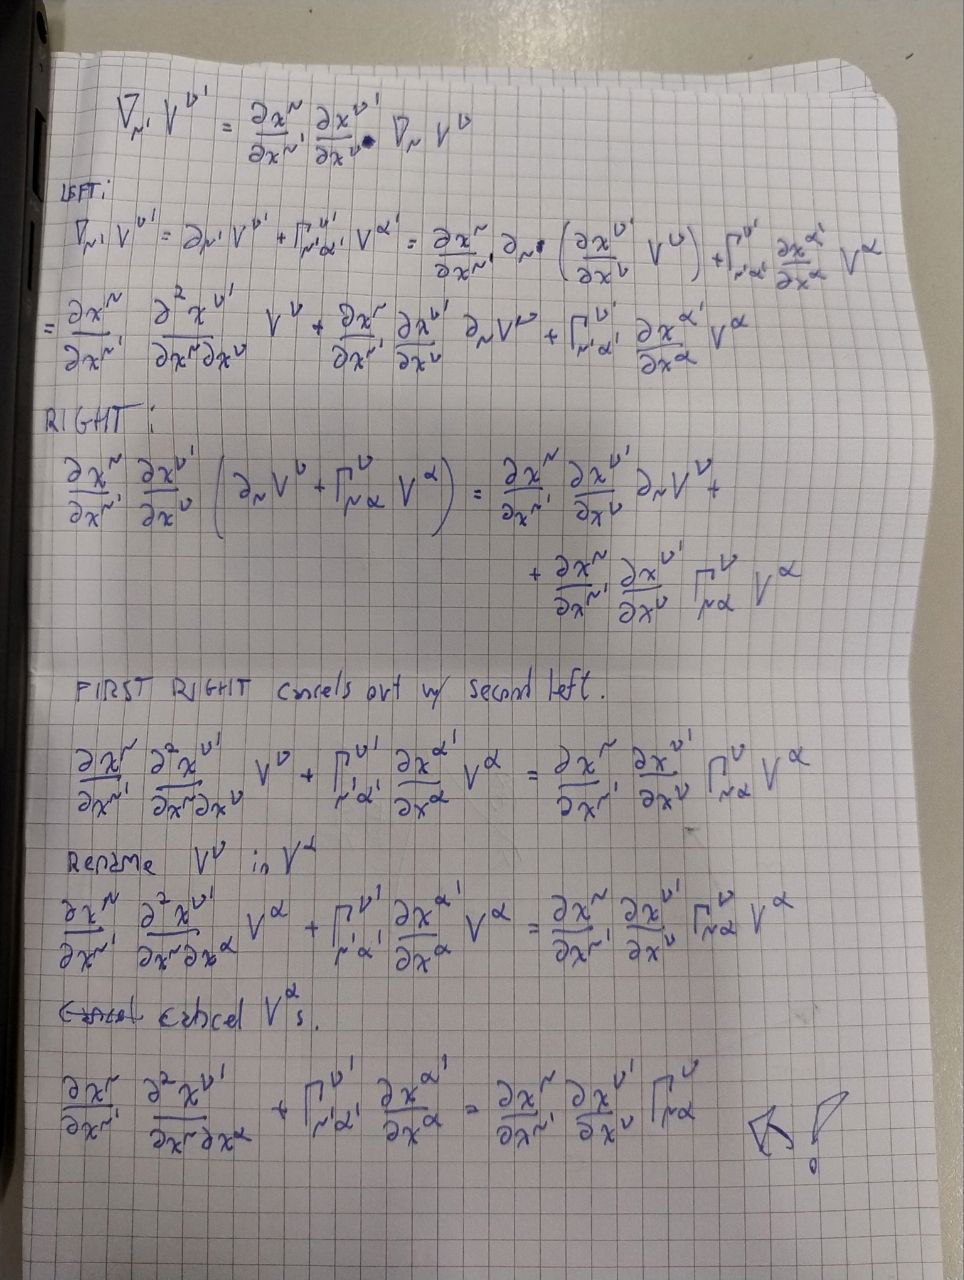
\includegraphics[width=0.8\linewidth]{imm/conntransf.jpg}
\caption{Same derivation but on paper. If you have any doubts compare with this one.}
\label{imm:conntransf}
\end{figure}
We see that $\Gamma $ is not a tensor because of this extra piece after the transformation.\par

\paragraph{Covariant derivative - dual vector}
We saw that for a \emph{vector} the covariant derivative acts like
\[
\nabla_{\mu }V^{\nu } = \partial_{\mu }V^{\nu } + \Gamma ^{\nu }_{\mu \alpha }V^{\alpha }
\]
Instead for a \emph{dual vector} the derivative is defined as
\[
\nabla _{\mu} \omega _{\nu } \equiv \partial_{\mu }\omega _{\nu } + \tilde{\Gamma }^{\alpha }_{\mu \nu }\omega _{\alpha }
\]
The question that arises from this is obvious: \emph{how $\tilde{\Gamma }$ is related to $\Gamma $?}\par
Let's compute 
\[
\nabla _{\mu }\left( \omega _{\lambda }V^{\lambda } \right) = \partial_{\mu } \left( \omega _{\lambda }V^{\lambda } \right)
\]
This because the covariant derivative of a scalar \emph{is} the derivative of a scalar. So, applying the Leibniz Rule:
\begin{gather*}
\nabla _{\mu }V^{\lambda }\cdot \omega _{\lambda } + V^{\lambda }\nabla _{\mu }\omega _{\lambda } = \partial_{\mu }V^{\lambda }\omega _{\lambda } + V^{\lambda }\partial_{\mu }\omega _{\lambda } \\
\left( \partial_{\mu }V^{\lambda } + \Gamma ^{\lambda }_{\mu  \alpha }V^{\alpha } \right)\omega _{\lambda } + V^{\lambda }\left( \partial_{\mu }\omega _{\lambda } + \tilde{\Gamma }^{\alpha }_{\mu  \lambda } \omega _{\alpha } \right) = \left( \partial_{\mu }V^{\lambda } \right)\omega _{\lambda }+ \left( \partial_{\mu }\omega _{\lambda } \right)V^{\lambda }\\
\to  \Gamma ^{\lambda }_{\mu  \alpha }V^{\alpha }\omega _{\lambda } + \tilde{\Gamma }^{\alpha }_{\mu \lambda } V^{\lambda }\omega _{\alpha } = 0 \\
\text{ renaming some indices to get }\\
\Gamma ^{\lambda }_{\mu \alpha }V^{\alpha }\omega _{\lambda } + \tilde{\Gamma }^{\lambda }_{\mu  \alpha } V^{\alpha }\omega _{\lambda } \\
\implies \Gamma ^{\lambda }_{\mu \alpha } + \tilde{\Gamma }^{\lambda }_{\mu  \alpha } = 0
\end{gather*}

To conclude, the covariant derivative of a dual vector is actually
\begin{equation}
\nabla _{\mu }\omega_{\nu  }= \partial_{\mu }\omega _{\nu } - \Gamma ^{\alpha }_{\mu \nu }\omega _{\alpha }
\end{equation}
 
























\section{Lec 11}
\subsection{Covariant derivative - Connection}
In the last lecture we talked about the covariant derivative and we saw the version for the vector, for the dual vector, and how it transform between two coordinates systems. We constructed it so the output is a tensor, and we saw that even after changes of coordinates we still get a tensor.\par
The question now is, how to do
\[
\nabla _{\rho }T^{\mu _{1}\ldots \mu _{k}}_{\nu _{1}\ldots \nu _{l}} = ?
\]
The development is pretty boring but straight-forward:
\begin{equation}
= \partial_{\rho }T^{\mu_{1} \ldots \mu_{k}}_{\nu_{1} \ldots \nu_{l}} + \Gamma ^{\mu _{1}}_{\rho \alpha } T^{\alpha \mu_{2} \ldots \mu_{k}}_{\nu_{1} \ldots \nu_{l}} + \Gamma ^{\mu_{2}}_{\rho \alpha }T^{\mu_{1} \alpha \mu_{3} \ldots \mu_{k}}_{\nu_{1} \ldots \nu_{l}} + \ldots - \Gamma ^{\alpha }_{\mu \nu _{1}} T^{\mu _{1} \ldots \mu _{k}}_{\alpha \nu_{2} \ldots \nu_{l}} - \ldots 
\end{equation}
These $\Gamma $ connections are just tables of 64 entries of numbers, not tensors, and putting indices up and down to it it's abuse of notation. \par
Now we will make a couple of assumptions on the structure of $\Gamma $.
\subsubsection{Torsion}
\paragraph{Statement I} Given two different connections $\Gamma^{\mu }_{\alpha \beta }$ and $\tilde{\Gamma }^{\mu }_{\alpha \beta }$, we define
\[
S^{\mu }_{\alpha \beta } = \Gamma ^{\mu }_{\alpha \beta } - \tilde{\Gamma }^{\mu }_{\alpha \beta }	
\]
$\to  S^{\mu }_{\alpha \beta }$ is a (1,2) tensor. Why? Since I have
\[
\nabla _{\mu }V^{\nu } = \partial_{\mu }V^{\nu }+ \Gamma ^{\nu }_{\mu  \alpha }V^{\alpha }
\]
I can define a complement
\[
\tilde{\nabla }_{\mu }V^{\nu } = \partial_{\mu }V^{\nu } + \tilde{\Gamma }^{\nu }_{\mu \alpha }V^{\alpha }
\]
so i get
\[
\to  \nabla _{\mu }V^{\nu }- \tilde{\nabla }_{\mu }V^{\nu } = \left( \Gamma ^{\nu }_{\mu  \alpha } - \tilde{\Gamma }^{\nu }_{\mu  \alpha } \right)V^{\alpha } = S^{\nu }_{\mu  \alpha }V^{\alpha }
\]
and this is valid \emph{only} if $S^{\mu }_{\nu  \alpha }$ is a tensor.

\paragraph{Statement II} if $\Gamma ^{\mu }_{\alpha \beta }$ is a connection $\implies  \Gamma ^{\mu }_{\beta  \alpha }$ is a connection.\par
That's why we define the \emph{ Torsion tensor}
\[
	T^{\mu }_{\alpha \beta }\equiv \Gamma  ^{\mu }_{\alpha \beta } - \Gamma ^{\mu }_{\beta  \alpha } = 2 \Gamma ^{\mu }_{[\alpha \beta ]}
\]
The metric adopted in this course is a \emph{ Torsion-Free} metric, so the torsion tensor is vanishing.\par
How many entries do I have for a connection?
\[
\Gamma ^{\mu \to 4}_{\alpha \beta \to 10}
\]
so in total I have 40 entries, 4 for the upper index and 10 for the lowers because symmetry, \par

As we will see later, the name \emph{connection} comes from the fact that it is used to transport vectors from one tangent space to another.
\subsubsection{Metric Compatibility}
So, the torsion tensor is antisymmetric on its lower indices, and a connection that is symmetric on its lower indices is \emph{torsion-free}
We can define a unique connection on a manifold with metric $g_{\mu \nu }$ by introducing two additional properties, torsion-freeness and the metric compatibility.
The metric compatibility is a property of the covariant derivative and it's expressed as follows
\[
\nabla \rho g_{\mu \nu } = 0
\]
A connection is \emph{metric compatible} if the covariant derivative of the metric with respect to that connection is everywhere 0. \par
We want to see how this property works with the \emph{inverse metric tensor}, so let's start from
\begin{equation}
\nabla _{\rho } \left( g^{\alpha \beta } g_{\beta  \gamma } \right) =\nabla _{\rho } \left( \delta ^{\alpha }_{\gamma }  \right) = \Gamma ^{\alpha }_{\rho \lambda  }\delta^{\lambda }_{\gamma } - \Gamma ^{\sigma  }_{\rho \gamma }\delta^{\alpha }_{\sigma } + \partial_{\rho }\left( \delta ^{\alpha }_{\gamma } \right) = \left( \Gamma ^{\alpha }_{\rho  \gamma } - \Gamma ^{\alpha }_{\rho  \gamma } \right) = 0
\end{equation}
the term with the partial derivative cancels out because $\delta $ is constant, and we equal everything to zero because the covariant derivative of the Kronecker delta is 0. On the right side we can apply the Leibniz rule so
\begin{equation}
g^{\alpha \beta }\nabla _{\rho }\left( g_{\beta \gamma } \right) + \nabla _{\rho }\left( g^{\alpha \beta } \right)g_{\beta \gamma } = 0
\end{equation}
the first term is 0, because we said so, the connection is metric compatible. We are left with
\[
g_{\beta  \gamma }\nabla _{\rho }\left( g^{\alpha \beta } \right) = 0
\]
by multiplying on both sides $g^{\gamma \sigma }$
\[
g^{\gamma \sigma } g_{\beta \gamma } \nabla _{\rho } \left( g^{\alpha \beta } \right) =0
\]
I get
\[
\delta ^{\sigma }_{\beta }\nabla _{\rho }\left( g^{\alpha \beta } \right) = \nabla _{\rho }\left( \delta ^{\sigma }_{\beta } g^{\alpha \beta } \right) = \nabla _{\rho }\left( g^{\alpha \sigma } \right) = 0
\]
So, in conclusion the covariant derivative of the inverse of metric tensor is null. It was not trivial.

After this we can see that a metric-compatible covariant derivative commutes with raising and lowering of indices, so for a generic vector $V^{\nu }$
\[
\nabla _{\mu }V^{\nu } = g_{\alpha \nu }\nabla _{\mu }\left( v^{\mu } \right) = \nabla _{\mu }\left( g_{\alpha \nu }V^{\nu } \right) = \nabla _{\mu }V_{\nu }
\]

With non-metric compatible connections we would have to be very careful about index placement wen taking a covariant derivative. \par
There is exactly one torsion-free connection on a manifold that is compatible with some generic metric on that manifold. \par

We can demonstrate \emph{existence} and \emph{uniqueness} by deriving a manifestly unique expression for the connection coefficients in terms of the metric, so we will expand the equation of metric compatibility for three different permutations of the indices.
\begin{gather*}
\nabla _{\rho }g_{\mu \nu } = \partial_{\rho }g_{\mu \nu } - \Gamma ^{\lambda }_{\rho \mu }g_{ \lambda \nu  } - \Gamma ^{\lambda }_{\rho \nu } g_{\mu \lambda }=0  \text{ (a) }\\
\nabla _{\mu }g_{\nu \rho } = \partial_{\mu }g_{\nu \rho } - \Gamma ^{\lambda }_{\mu \nu }g_{\lambda \rho } - \Gamma ^{\lambda }_{\mu \rho }g_{\nu \lambda } =0 \text{ (b) }\\
\nabla _{\nu }g_{\rho \mu } = \partial_{\nu }g_{\rho \mu } - \Gamma ^{\lambda }_{\nu \rho } g_{\lambda \mu } - \Gamma ^{\lambda }_{\nu \mu } g_{\rho  \lambda } = 0 \text{ (c) }
\end{gather*}
we see that \emph{(a)-(b)-(c) = 0}, and it is obvious because individually they're equal to 0. \par
But let's see in detail what's happening
\begin{gather*}
\partial_{\rho }g_{\mu \nu } - \partial_{\mu }g_{\nu \rho } - \partial_{\nu }g_{\rho \mu } - \colorbox{yellow}{$ \Gamma^{\alpha }_{\rho \mu }g_{\alpha \nu }  $} - \colorbox{green}{$ \Gamma ^{\alpha }_{\rho \nu }g_{\mu \alpha }  $} + \\
 + \Gamma ^{\alpha }_{\mu \nu }g_{\alpha \rho } + \colorbox{yellow}{$ \Gamma^{\alpha }_{\mu \rho }g_{\nu \alpha }  $} + \colorbox{green}{$ \Gamma ^{\alpha }_{\nu \rho }g_{\alpha \mu }  $} + \Gamma ^{\alpha }_{\nu \mu }g_{\rho \alpha } = 0 \\
\end{gather*}
 We subtract the highlighted ones and use the symmetry of the connection to get
 \[
 2g_{\rho \alpha }\Gamma ^{\alpha }_{\mu \nu } - \partial_{\mu }g_{\nu \rho } + \partial_{\nu }g_{\mu \rho } - \partial_{\rho }g_{\mu \nu }
 \]
 We multiply both sides by $g^{\rho \sigma }$	
\begin{equation}
	\Gamma^{\sigma }_{\mu \nu } = \frac{1}{2} g^{\rho \sigma } [\partial_{\mu } g_{\nu \rho } + \partial_{\nu } g_{\mu \rho } - \partial_{\rho }g_{\mu \nu } ]
\end{equation}
 This is one of the most important expressions of the course. \par
 We have seen that a flat spacetime has a Minkowski metric everywhere. \par
 But how to define curvature? \par
 The fact that $g_{\mu \nu }$ depends on the coordinates is not enough (e.g. spherical coordinates). But now we have a new object\par
 Let's think a little bit: in flat spacetime if $\partial \leftrightarrow \nabla $ and this $\implies \Gamma  = 0$. Is that true? \par
 
 In 3D coordinates, using other coordinates, do connections have to be 0? Be
 \[
 \overline{\nabla } = \left( \frac{\partial }{\partial x} , \frac{\partial }{\partial y}  \right)
 \]
 that's the gradient in cartesian coordinates, but in polar coordinates
 \[
 = \left( \frac{\partial }{\partial r} , \frac{1}{r} \frac{\partial }{\partial \theta }  \right)
 \]
 I can compute the additional factor with christoffel symbols.
 Take $ds^{2} = dr^{2} + r^{2}d\theta ^{2}$, polar coordinates on plane, and compute the christoffel symbol. How many entries?
 \[
 \Gamma ^{\alpha \to 2}_{\beta \gamma \to 3} 
 \]
 I don't remember what the professor was trying to say but in doubt see Carroll.

 \subsection{Parallel Transport}
 


\tikzset{every picture/.style={line width=0.75pt}} %set default line width to 0.75pt        

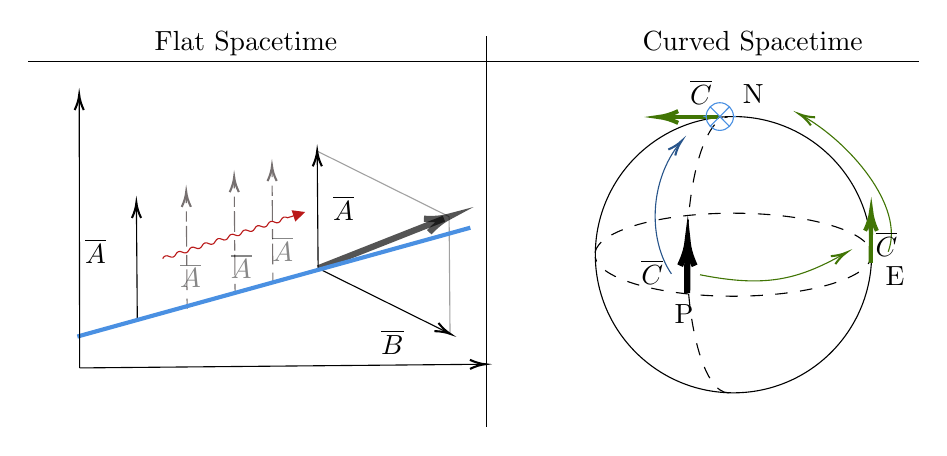
\begin{tikzpicture}[x=0.50pt,y=0.50pt,yscale=-1,xscale=1]
%uncomment if require: \path (0,300); %set diagram left start at 0, and has height of 300

%Straight Lines [id:da7804419238627388] 
\draw    (350.5,11.25) -- (350.5,294) ;
%Straight Lines [id:da6280355665081884] 
\draw    (19.5,29.25) -- (663,29.25) ;
%Straight Lines [id:da4130726982439956] 
\draw    (98.33,216.33) -- (97.68,133.67) ;
\draw [shift={(97.67,131.67)}, rotate = 89.55] [color={rgb, 255:red, 0; green, 0; blue, 0 }  ][line width=0.75]    (10.93,-3.29) .. controls (6.95,-1.4) and (3.31,-0.3) .. (0,0) .. controls (3.31,0.3) and (6.95,1.4) .. (10.93,3.29)   ;
%Straight Lines [id:da4487944386747611] 
\draw    (229,179) -- (228.35,96.33) ;
\draw [shift={(228.33,94.33)}, rotate = 89.55] [color={rgb, 255:red, 0; green, 0; blue, 0 }  ][line width=0.75]    (10.93,-3.29) .. controls (6.95,-1.4) and (3.31,-0.3) .. (0,0) .. controls (3.31,0.3) and (6.95,1.4) .. (10.93,3.29)   ;
%Straight Lines [id:da34584707728272546] 
\draw [color={rgb, 255:red, 118; green, 112; blue, 112 }  ,draw opacity=1 ] [dash pattern={on 3.75pt off 3pt on 7.5pt off 1.5pt}]  (134.33,208.33) -- (133.68,125.67) ;
\draw [shift={(133.67,123.67)}, rotate = 89.55] [color={rgb, 255:red, 118; green, 112; blue, 112 }  ,draw opacity=1 ][line width=0.75]    (10.93,-3.29) .. controls (6.95,-1.4) and (3.31,-0.3) .. (0,0) .. controls (3.31,0.3) and (6.95,1.4) .. (10.93,3.29)   ;
%Straight Lines [id:da8607896715027422] 
\draw [color={rgb, 255:red, 118; green, 112; blue, 112 }  ,draw opacity=1 ] [dash pattern={on 3.75pt off 3pt on 7.5pt off 1.5pt}]  (169,197.67) -- (168.35,115) ;
\draw [shift={(168.33,113)}, rotate = 89.55] [color={rgb, 255:red, 118; green, 112; blue, 112 }  ,draw opacity=1 ][line width=0.75]    (10.93,-3.29) .. controls (6.95,-1.4) and (3.31,-0.3) .. (0,0) .. controls (3.31,0.3) and (6.95,1.4) .. (10.93,3.29)   ;
%Straight Lines [id:da18547678451320238] 
\draw [color={rgb, 255:red, 118; green, 112; blue, 112 }  ,draw opacity=1 ] [dash pattern={on 3.75pt off 3pt on 7.5pt off 1.5pt}]  (196.33,189.67) -- (195.68,107) ;
\draw [shift={(195.67,105)}, rotate = 89.55] [color={rgb, 255:red, 118; green, 112; blue, 112 }  ,draw opacity=1 ][line width=0.75]    (10.93,-3.29) .. controls (6.95,-1.4) and (3.31,-0.3) .. (0,0) .. controls (3.31,0.3) and (6.95,1.4) .. (10.93,3.29)   ;
%Straight Lines [id:da6531580304035787] 
\draw [color={rgb, 255:red, 186; green, 25; blue, 25 }  ,draw opacity=1 ]   (116.67,172) .. controls (117.74,169.9) and (119.32,169.38) .. (121.42,170.45) .. controls (123.53,171.52) and (125.11,171) .. (126.17,168.89) .. controls (127.24,166.79) and (128.82,166.27) .. (130.92,167.34) .. controls (133.02,168.41) and (134.61,167.89) .. (135.68,165.79) .. controls (136.74,163.68) and (138.32,163.16) .. (140.43,164.23) .. controls (142.53,165.3) and (144.11,164.78) .. (145.18,162.68) .. controls (146.25,160.58) and (147.83,160.06) .. (149.93,161.13) .. controls (152.04,162.2) and (153.62,161.68) .. (154.69,159.57) .. controls (155.76,157.47) and (157.34,156.95) .. (159.44,158.02) .. controls (161.54,159.09) and (163.12,158.57) .. (164.19,156.47) .. controls (165.25,154.36) and (166.83,153.84) .. (168.94,154.91) .. controls (171.04,155.98) and (172.63,155.46) .. (173.7,153.36) .. controls (174.77,151.26) and (176.35,150.74) .. (178.45,151.81) .. controls (180.56,152.88) and (182.14,152.36) .. (183.2,150.25) .. controls (184.27,148.15) and (185.86,147.63) .. (187.96,148.7) .. controls (190.06,149.77) and (191.64,149.25) .. (192.71,147.15) .. controls (193.77,145.04) and (195.35,144.52) .. (197.46,145.59) .. controls (199.56,146.66) and (201.14,146.14) .. (202.21,144.04) .. controls (203.28,141.93) and (204.86,141.41) .. (206.97,142.48) -- (209.21,141.75) -- (216.82,139.27) ;
\draw [shift={(219.67,138.33)}, rotate = 161.9] [fill={rgb, 255:red, 186; green, 25; blue, 25 }  ,fill opacity=1 ][line width=0.08]  [draw opacity=0] (8.93,-4.29) -- (0,0) -- (8.93,4.29) -- cycle    ;
%Straight Lines [id:da096404784455415] 
\draw    (229,179) -- (322.54,225.44) ;
\draw [shift={(324.33,226.33)}, rotate = 206.4] [color={rgb, 255:red, 0; green, 0; blue, 0 }  ][line width=0.75]    (10.93,-3.29) .. controls (6.95,-1.4) and (3.31,-0.3) .. (0,0) .. controls (3.31,0.3) and (6.95,1.4) .. (10.93,3.29)   ;
%Straight Lines [id:da31708594059819595] 
\draw [color={rgb, 255:red, 0; green, 0; blue, 0 }  ,draw opacity=0.37 ]   (228.33,94.33) -- (323.67,141.67) ;
%Straight Lines [id:da44013896128415253] 
\draw [color={rgb, 255:red, 0; green, 0; blue, 0 }  ,draw opacity=0.37 ]   (324.33,226.33) -- (323.67,141.67) ;
%Straight Lines [id:da693791852252502] 
\draw [color={rgb, 255:red, 0; green, 0; blue, 0 }  ,draw opacity=0.67 ][line width=2.25]    (229,179) -- (319.95,143.13) ;
\draw [shift={(323.67,141.67)}, rotate = 158.48] [color={rgb, 255:red, 0; green, 0; blue, 0 }  ,draw opacity=0.67 ][line width=2.25]    (17.49,-5.26) .. controls (11.12,-2.23) and (5.29,-0.48) .. (0,0) .. controls (5.29,0.48) and (11.12,2.23) .. (17.49,5.26)   ;
%Shape: Circle [id:dp9665324253206228] 
\draw   (429.33,169.17) .. controls (429.33,114.03) and (474.03,69.33) .. (529.17,69.33) .. controls (584.3,69.33) and (629,114.03) .. (629,169.17) .. controls (629,224.3) and (584.3,269) .. (529.17,269) .. controls (474.03,269) and (429.33,224.3) .. (429.33,169.17) -- cycle ;
%Shape: Arc [id:dp9307781681306638] 
\draw  [draw opacity=0][dash pattern={on 4.5pt off 4.5pt}] (429.12,167.7) .. controls (431.66,151.81) and (475.41,139.17) .. (529,139.17) .. controls (584.23,139.17) and (629,152.6) .. (629,169.17) .. controls (629,185.74) and (584.23,199.17) .. (529,199.17) .. controls (475.9,199.17) and (432.46,186.75) .. (429.2,171.07) -- (529,169.17) -- cycle ; \draw  [dash pattern={on 4.5pt off 4.5pt}] (429.12,167.7) .. controls (431.66,151.81) and (475.41,139.17) .. (529,139.17) .. controls (584.23,139.17) and (629,152.6) .. (629,169.17) .. controls (629,185.74) and (584.23,199.17) .. (529,199.17) .. controls (475.9,199.17) and (432.46,186.75) .. (429.2,171.07) ;  
%Shape: Arc [id:dp9109349274225841] 
\draw  [draw opacity=0][dash pattern={on 4.5pt off 4.5pt}] (525.66,269) .. controls (525.63,269) and (525.6,269) .. (525.57,269) .. controls (509,269) and (495.57,224.35) .. (495.57,169.27) .. controls (495.57,114.74) and (508.73,70.44) .. (525.07,69.55) -- (525.57,169.27) -- cycle ; \draw  [dash pattern={on 4.5pt off 4.5pt}] (525.66,269) .. controls (525.63,269) and (525.6,269) .. (525.57,269) .. controls (509,269) and (495.57,224.35) .. (495.57,169.27) .. controls (495.57,114.74) and (508.73,70.44) .. (525.07,69.55) ;  
%Straight Lines [id:da9377226925217493] 
\draw [line width=2.25]    (495.67,197) -- (495.96,163.67) ;
\draw [shift={(496,159.67)}, rotate = 90.51] [color={rgb, 255:red, 0; green, 0; blue, 0 }  ][line width=2.25]    (17.49,-5.26) .. controls (11.12,-2.23) and (5.29,-0.48) .. (0,0) .. controls (5.29,0.48) and (11.12,2.23) .. (17.49,5.26)   ;
%Curve Lines [id:da248689634217361] 
\draw [color={rgb, 255:red, 65; green, 117; blue, 5 }  ,draw opacity=1 ]   (505,183.67) .. controls (551.62,192.86) and (574.96,187.82) .. (609.1,168.56) ;
\draw [shift={(610.67,167.67)}, rotate = 150.26] [color={rgb, 255:red, 65; green, 117; blue, 5 }  ,draw opacity=1 ][line width=0.75]    (10.93,-3.29) .. controls (6.95,-1.4) and (3.31,-0.3) .. (0,0) .. controls (3.31,0.3) and (6.95,1.4) .. (10.93,3.29)   ;
%Curve Lines [id:da3715785341810326] 
\draw [color={rgb, 255:red, 40; green, 85; blue, 139 }  ,draw opacity=1 ]   (484.33,183) .. controls (467.26,158.05) and (468.3,115.63) .. (490.63,88.24) ;
\draw [shift={(491.67,87)}, rotate = 130.49] [color={rgb, 255:red, 40; green, 85; blue, 139 }  ,draw opacity=1 ][line width=0.75]    (10.93,-3.29) .. controls (6.95,-1.4) and (3.31,-0.3) .. (0,0) .. controls (3.31,0.3) and (6.95,1.4) .. (10.93,3.29)   ;
%Curve Lines [id:da33000822429954535] 
\draw [color={rgb, 255:red, 65; green, 117; blue, 5 }  ,draw opacity=1 ]   (641,167) .. controls (653.48,134.17) and (612.27,87.1) .. (578.54,68.5) ;
\draw [shift={(577,67.67)}, rotate = 27.9] [color={rgb, 255:red, 65; green, 117; blue, 5 }  ,draw opacity=1 ][line width=0.75]    (10.93,-3.29) .. controls (6.95,-1.4) and (3.31,-0.3) .. (0,0) .. controls (3.31,0.3) and (6.95,1.4) .. (10.93,3.29)   ;
%Straight Lines [id:da11933692361161596] 
\draw [color={rgb, 255:red, 65; green, 117; blue, 5 }  ,draw opacity=1 ][line width=1.5]    (628.33,175) -- (628.64,140.67) ;
\draw [shift={(628.67,137.67)}, rotate = 90.51] [color={rgb, 255:red, 65; green, 117; blue, 5 }  ,draw opacity=1 ][line width=1.5]    (14.21,-4.28) .. controls (9.04,-1.82) and (4.3,-0.39) .. (0,0) .. controls (4.3,0.39) and (9.04,1.82) .. (14.21,4.28)   ;
%Straight Lines [id:da9460218080051334] 
\draw [color={rgb, 255:red, 65; green, 117; blue, 5 }  ,draw opacity=1 ][line width=1.5]    (519,69.67) -- (478,69.67) ;
\draw [shift={(475,69.67)}, rotate = 360] [color={rgb, 255:red, 65; green, 117; blue, 5 }  ,draw opacity=1 ][line width=1.5]    (14.21,-4.28) .. controls (9.04,-1.82) and (4.3,-0.39) .. (0,0) .. controls (4.3,0.39) and (9.04,1.82) .. (14.21,4.28)   ;
%Shape: Light Bulb [id:dp7648536590068119] 
\draw  [color={rgb, 255:red, 74; green, 144; blue, 226 }  ,draw opacity=1 ] (509.44,69.33) .. controls (509.44,63.81) and (513.86,59.33) .. (519.31,59.33) .. controls (524.75,59.33) and (529.17,63.81) .. (529.17,69.33) .. controls (529.17,74.86) and (524.75,79.33) .. (519.31,79.33) .. controls (513.86,79.33) and (509.44,74.86) .. (509.44,69.33) -- cycle (512.28,62.21) -- (526.33,76.45) (526.33,62.21) -- (512.28,76.45) (507.47,69.33) -- (509.44,69.33) (529.17,69.33) -- (531.14,69.33) ;
%Straight Lines [id:da26085572297009496] 
\draw [color={rgb, 255:red, 74; green, 144; blue, 226 }  ,draw opacity=1 ][line width=1.5]    (55,228.33) -- (339,149.67) ;
%Straight Lines [id:da17265066162065923] 
\draw    (56.67,251) -- (56.34,55.67) ;
\draw [shift={(56.33,53.67)}, rotate = 89.9] [color={rgb, 255:red, 0; green, 0; blue, 0 }  ][line width=0.75]    (10.93,-3.29) .. controls (6.95,-1.4) and (3.31,-0.3) .. (0,0) .. controls (3.31,0.3) and (6.95,1.4) .. (10.93,3.29)   ;
%Straight Lines [id:da8026826708800486] 
\draw    (56.67,251) -- (347.67,248.35) ;
\draw [shift={(349.67,248.33)}, rotate = 179.48] [color={rgb, 255:red, 0; green, 0; blue, 0 }  ][line width=0.75]    (10.93,-3.29) .. controls (6.95,-1.4) and (3.31,-0.3) .. (0,0) .. controls (3.31,0.3) and (6.95,1.4) .. (10.93,3.29)   ;

% Text Node
\draw (109,5.5) node [anchor=north west][inner sep=0.75pt]   [align=left] {Flat Spacetime};
% Text Node
\draw (461.67,5.67) node [anchor=north west][inner sep=0.75pt]   [align=left] {Curved Spacetime};
% Text Node
\draw (58.67,155.67) node [anchor=north west][inner sep=0.75pt]   [align=left] {$\displaystyle \overline{A}$};
% Text Node
\draw (238,125) node [anchor=north west][inner sep=0.75pt]   [align=left] {$\displaystyle \overline{A}$};
% Text Node
\draw (127.33,173.67) node [anchor=north west][inner sep=0.75pt]  [color={rgb, 255:red, 0; green, 0; blue, 0 }  ,opacity=0.47 ] [align=left] {$\displaystyle \overline{A}$};
% Text Node
\draw (164,167) node [anchor=north west][inner sep=0.75pt]  [color={rgb, 255:red, 0; green, 0; blue, 0 }  ,opacity=0.47 ] [align=left] {$\displaystyle \overline{A}$};
% Text Node
\draw (194,154.33) node [anchor=north west][inner sep=0.75pt]  [color={rgb, 255:red, 0; green, 0; blue, 0 }  ,opacity=0.47 ] [align=left] {$\displaystyle \overline{A}$};
% Text Node
\draw (272.67,221.67) node [anchor=north west][inner sep=0.75pt]   [align=left] {$\displaystyle \overline{B}$};
% Text Node
\draw (484.67,203) node [anchor=north west][inner sep=0.75pt]   [align=left] {P};
% Text Node
\draw (534,44.67) node [anchor=north west][inner sep=0.75pt]   [align=left] {N};
% Text Node
\draw (637.33,176) node [anchor=north west][inner sep=0.75pt]   [align=left] {E};
% Text Node
\draw (460.67,171) node [anchor=north west][inner sep=0.75pt]   [align=left] {$\displaystyle \overline{C}$};
% Text Node
\draw (630,151) node [anchor=north west][inner sep=0.75pt]   [align=left] {$\displaystyle \overline{C}$};
% Text Node
\draw (496,41) node [anchor=north west][inner sep=0.75pt]   [align=left] {$\displaystyle \overline{C}$};
\end{tikzpicture}

In flat spacetime, if we want to add $\overline{A}+ \overline{B}$, we move the $\overline{A}$ vector along the blue line. We \emph{can} move $\overline{A}$ also along a non-straight line but $\overline{A}$ remains $\overline{A}$, and for the sum I get the same result.\par
In flat spacetime parallel transport does not depend on the path.\par

In curved spacetime, if I move $\overline{C}$ from \emph{P} to \emph{N} along the geodesic, we get that $\overline{C}$ points inside the sheet. But if I choose another path like \emph{P-E-N}, then the outcome is a vector $\overline{C}$ that points toward left. It's not the same vector. \par
In curved spacetime parallel transport depends on the trajectory, we have to specify the path.\par
Be the path $x^{\mu }\left( \lambda  \right) : \mathbb{R} \to \text{ spacetime coordinates }$. In FST parallel transportation of a generic tensor is
\[
\frac{d}{d\lambda } \left( T^{\mu _{1} \ldots \mu _{l}}_{\nu _{1}\ldots \nu _{l}} \right) = 0
\]
and the first factor is the directional derivative. Or
\[
\frac{d x^{\sigma }}{d \lambda } \partial_{\sigma } \left( T^{\mu _{1}\ldots \mu _{k}}_{\nu _{1}\ldots \nu _{l}} \right) = 0
\]
While in CST:
\[
\frac{dx^{\sigma }}{d\lambda } \nabla _{\sigma } \left(T^{\mu _{1}\ldots \mu _{k}}_{\nu _{1}\ldots \nu _{l}} \right) = 0
\]
Let's see a simple example: imagine we have $x^{\mu }\left( \lambda  \right) = \left( \lambda , 0, 0 , 0 \right)$ so $x^{\mu }\left( 0 \right) = \left( 0,0,0,0 \right)$ and the four velocity is $V^{\mu }\left( 0 \right) = \left( 1,0,0,0 \right)$.
In FST 
\[
\frac{dx^{\sigma }}{d\lambda } \left( \partial_{\sigma }V^{\mu } \right) = \frac{dx^{0}}{d\lambda } \partial_{0}V^{\mu } = \partial_{0}V^{\mu } = 0
\]
The vector does not change. \par

Why is it useful? Let's introduce
\subsubsection{Geodesics}
They are a straight line in curved space, the trajectory of a particle only subject to gravity. With \emph{straight line} we mean the path that is parallel transported along it's tangent vector.

\textbf{Example} In FST we have a vector that have the same direction of a straight line, and we want to move it along that line. 
So if I transport the vector tangent to the line, I get the same line.

\tikzset{every picture/.style={line width=0.75pt}}\label{imm:straigthline}

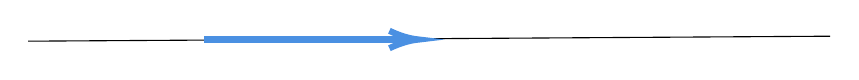
\begin{tikzpicture}[x=0.60pt,y=0.60pt,yscale=-1,xscale=1]
%uncomment if require: \path (0,300); %set diagram left start at 0, and has height of 300

%Straight Lines [id:da7933369365137976]
\draw    (100,106) -- (583,103) ;
%Straight Lines [id:da5367435588258249]
\draw [color={rgb, 255:red, 74; green, 144; blue, 226 }  ,draw opacity=1 ][line width=2.25]    (206,105) -- (331,105) ;
\draw [shift={(335,105)}, rotate = 180] [color={rgb, 255:red, 74; green, 144; blue, 226 }  ,draw opacity=1 ][line width=2.25]    (17.49,-5.26) .. controls (11.12,-2.23) and (5.29,-0.48) .. (0,0) .. controls (5.29,0.48) and (11.12,2.23) .. (17.49,5.26)   ;
\end{tikzpicture} \par
In CST, with path $x^{\mu }\left( \lambda  \right)$, we have tangent
\[
\frac{dx^{\mu }}{d\lambda  }
\]
and that gives
\[
\frac{dx^{\sigma }}{d\lambda } \nabla _{\sigma } \left( \frac{dx^{\mu }}{d\lambda } \right) = 0
\]
It's a geodesics if this last condition is satisfied.
Let's focus on this
\begin{gather*}
	\frac{dx^{\sigma }}{d\lambda } \left[ \frac{\partial }{\partial x^{\sigma }}  \frac{dx^{\mu }}{d\lambda } + \Gamma ^{\mu }_{\sigma \alpha } \frac{dx^{\alpha }}{d\lambda }\right] = 0 \\
\to  \frac{d^{2}x^{\mu }}{d\lambda } + \Gamma^{\mu }_{\alpha \beta } \frac{dx^{\alpha }}{d\lambda } \frac{d x^{\beta }}{d\lambda } = 0
\end{gather*}
the last one is the \emph{geodesics equation}, and it's very important. \par

Suggested exercise: do that in polar coordinates in FST.
















\section{Lec 12}
\subsection{Geodesic Equation}
Given a generic path (WL) $x^{\mu }\left( \lambda  \right)$, parallel transport of a generic tensor is
\[
\frac{D}{d\lambda } \left( T^{\mu _{1}\ldots \mu _{k}}_{\nu _{1}\ldots \nu _{l}}\right) =\frac{d x^{\sigma }}{d \lambda } \nabla _{\sigma } T^{\mu _{1}\ldots \mu _{k}}_{\nu _{1}\ldots \nu _{l}} = 0		
\]
while for a vector is 
\[
	\frac{D}{d\lambda } \left( V^{\rho } \right) = \frac{d x^{\mu }}{d \lambda } \nabla _{\mu }V^{\rho } = \frac{d x^{\mu }}{d \lambda } \left[ \partial_{\mu }V^{\rho } + \Gamma ^{\rho }_{\mu \sigma  } V^{\sigma } \right]=0
\]
We can look at the parallel transport equations as a first-order differential equation defining an initial-value problem: given a tensor at some point along the path, there will be a unique continuation of the tensor to other points along the path.

Probably it was not said before but to make the parallel transport properly tensorial we need to replace the partial derivative by a covariant one, and define the \emph{directional covariant derivative} as
\[
\frac{D}{d\lambda } = \frac{d x^{\mu }}{d \lambda }\nabla _{\mu }
\]

We will review \emph{geodesic equation} and derive it again with a different method.

\subsubsection{Geodesic I}
Geodesic is a path that transport its own tangent vector. That's the definition we will use for the first method. We schematized this in Lec 11, fig. \ref{imm:straigthline}.

\begin{gather*}
\frac{D}{d\lambda } \left( \frac{d x^{\mu }}{d \lambda } \right) = 0 \\
\to  \frac{d x^{\sigma }}{d \lambda }\nabla _{\sigma }\left( \frac{d x^{\mu }}{d \lambda } \right) = \frac{d x^{\sigma }}{d \lambda }\left[ \partial_{\sigma } \left( \frac{d x^{\mu }}{d \lambda } \right) + \Gamma ^{\mu }_{\sigma \rho } \frac{d x^{\rho }}{d \lambda } \right] = 0 \\
\to \frac{d ^{2} x^{\mu }}{d \lambda ^{2}} + \Gamma ^{\mu }_{\rho \sigma } \frac{d x^{\rho }}{d \lambda } \frac{d x^{\sigma }}{d \lambda } = 0 
\end{gather*}
so we get the \emph{geodesic equation.}

\subsubsection{Geodesic II}

This time let's start from the concept of distance so
\[
ds^{2} = g_{\mu \nu } dx^{\mu }dx^{\nu }
\]
There is no point in trying to minimize it, because if it's the path of a photon it is 0, it's already minimized for each null-path.\par
Since the metric is compatible with the connection we are using, we take the parallel transportation of this quantity, that is a scalar, $g_{\mu \nu }V^{\mu }W^{\nu }$:
\begin{equation}
\frac{D}{d\lambda } \left( g_{\mu \nu }V^{\mu }W^{\nu }	 \right) = \left( \frac{D}{d\lambda } g_{\mu \nu } \right)V^{\mu }W^{\nu } + g_{\mu \nu } \frac{D}{d\lambda }\left( V^{\mu }\right)W^{\nu }+ g_{\mu \nu} V^{\mu } \frac{D }{d \lambda } \left( W^{\nu } \right)
\end{equation}
we see that the first term on the right is 0 because of \emph{metric compatibility} and the other two are 0 as well because we are parallel transporting a vector\footnote{and the vector does not change}.\par
What does it mean? It means that scalar product is preserved by parallel transportation.\par
We will keep this lemma in mind while deriving the Geodesics Equation.

Now since in Lorentzian spacetime the definition of distance is kinda tricky let's stick to use proper time $\tau $, instead. So for a time-like trajectory, like the one of a massive particle, we have
\[
d\tau ^{2}= -g_{\mu \nu }dx^{\mu }dx^{\nu } \text{ and } d\tau ^{2}> 0
\]
For every trajectory we fix the extremes so we get the so-called \emph{proper time functional}
\[
\tau \equiv \int_{path}^{}\sqrt{-g_{\mu \nu } \frac{d x^{\mu }}{d \lambda } \frac{d x^{\nu }}{d \lambda }} d\lambda 	
\]
To search for the shortest distance one could do a thing called \emph{calculus of variations} or alternatively, recalling the twin paradox, recognize that the twin that experience more time is the one who stands still on the Earth. But we will try to check this out anyway.  We can simplify the algebra writing the integral above as
\begin{gather*}
	\tau  \equiv \int_{path}^{}{\sqrt{-f} d\lambda } \\
	\text{ with } f = g_{\mu \nu } \frac{d x^{\mu }}{d \lambda } \frac{d x^{\nu }}{d \lambda }.
\end{gather*}
Then we add perturbations to the path, and we pick the one with the maximum proper time.

To extremize the proper time functional, we need that its variation is null. This implies that the tangent vector to the path $\frac{d x^{\mu }}{d \lambda }$, behaves consistently along the curve. This vector is normalized such that the scalar product \emph{f} is constant, and the fact that parallel transport preserves the scalar product guarantees that this holds along the path.\par
i%So, extremes called A and B are fixed, we took a generic trajectory $x^{\mu }\left( \lambda  \right)$.
We consider a \emph{perturbation} of this trajectory such that
\begin{gather*}
x^{\mu  }\to x^{\mu }\delta x^{\mu } \\
g_{\mu \nu } \to  g_{\mu \nu } + \partial_{\rho }g_{\mu \nu } \delta  x^{\rho }
\end{gather*}
Where the second line comes from Taylor expansion in CST, which uses partial derivative not covariant one, because we are thinking of the components of $g_{\mu \nu }$ as functions of spacetime in some specific coordinates system.
Since we modify the trajectory, $\tau$ also changes
\[
	\delta \tau = \int_{}^{}{\delta \sqrt{-f}d\lambda } = \int_{}^{}{-\frac{1}{2\sqrt{-f}}\delta f d\lambda }
\]
Now we switch parameter to $\tau $ itself, this makes the four-velocity to become the tangent vector, and consequently the value of \emph{f} is now fixed at 
\[
f = g_{\mu \nu }\frac{d x^{\mu }}{d \tau }\frac{d x^{\nu }}{d \tau } = g_{\mu \nu }U^{\mu }U^{\nu } = -1
\]
and so
\[
\delta \tau = -\frac{1}{2} \int_{}^{}{\delta f d\tau }
\]
Stationary points of the \emph{functional of the proper time}, ( path for which $\delta  \tau =0$), are equivalent to stationary points of this simpler integral
\[
I = \frac{1}{2} \int_{}^{}{f d\tau } = \frac{1}{2} \int_{}^{}{g_{\mu \nu }\frac{d x^{\mu }}{d \lambda }\frac{d x^{\nu }}{d \lambda }}
\]
adding the perturbations on \emph{I} gets us
\begin{gather}\label{eq:deltaI}
\delta I = \frac{1}{2} \int_{}^{}{\left( \partial_{\sigma }g_{\mu \nu }\frac{d x^{\mu }}{d \tau }\frac{d x^{\nu }}{d \tau }\delta x^{\sigma } + g_{\mu \nu } \frac{d \left( \delta x^{\mu } \right)}{d \tau }\frac{d x^{\nu }}{d \tau } + g_{\mu \nu }\frac{d x_{\mu }}{d \tau } \frac{d \left(\delta  x^{\nu } \right)}{d \tau } \right)d\tau } \\
= \frac{1}{2} \int_{}^{}{\left( \partial_{\rho }g_{\mu \nu }\delta x^{\rho } \frac{d x^{\mu }}{d \tau } \frac{d x^{\nu }}{d \tau } +  g_{\mu \nu }\frac{d }{d \tau } \delta \left( x^{\mu } \right) \frac{d x^{\nu }}{d \tau } + g_{\mu \nu } \frac{d x^{\mu }}{d \tau } \frac{d }{d \tau } \delta \left( x^{\nu } \right) \right) d\tau }
\end{gather}
The last two terms can be integrated by parts,
\begin{gather*}
	\int_{}^{}{g_{\mu \nu } \frac{d }{d \tau }\left( \delta x^{\mu } \right) \frac{d x^{\nu }}{d \tau } d\tau } = \text{ boundary term } - \int_{}^{}{\frac{d }{d \tau } \left( g_{\mu \nu }\frac{d x^{\nu }}{d \tau } \right) \delta x^{\mu } d\tau } \\
 = - \int_{}^{}{\left( \partial_{\rho }g_{\mu \nu } \frac{d x^{\rho }}{d \tau } \frac{d x^{\nu }}{d \tau } + g_{\mu \nu } \frac{d ^{2} x^{\nu }}{d \tau ^{2}} \right) \delta x^{\mu } d\tau }
\end{gather*}
the boundary term vanishes because we take our variation $\delta x^{\mu }$ to vanish at the endpoints of the path. \par
So now we can insert back what we found in eq. \ref{eq:deltaI}
\begin{gather*}
\delta I = \frac{1}{2} \int_{}^{}{\partial_{\rho }g_{\mu \nu } \frac{d x^{\nu }}{d \tau } \frac{d x^{\mu  }}{d \tau } \delta x^{\rho } d\tau } - \frac{1}{2} \int_{}^{}{\left( \partial_{\rho } g_{\mu \nu } \frac{d x^{\rho }}{d \tau } \frac{d x^{\nu }}{d \tau } + g_{\mu \nu } \frac{d ^{2}x^{\nu }}{d \tau ^{2}} \right) \delta x^{\mu }d\tau }  +\\
- \frac{1}{2} \int_{}^{}{\left( \partial_{\rho } g_{\mu \nu } \frac{d x^{\rho }}{d \tau } \frac{d x^{\mu }}{d \tau } + g_{\mu \nu } \frac{d ^{2} x^{\mu }}{d \tau ^{2}} \right) \delta x^{\nu } d\tau }
\end{gather*}
We can make things easier if we use:
\begin{itemize}
\item $\alpha $ instead of $\rho $ in the first term
\item $\alpha $ instead of $\mu $ in the second term
\item $\alpha $ instead of $\nu $ in the third term
\item $\rho $ in second term is now $\mu $
\item $\rho $ in third term is now $\nu $
\item $\nu $ in one derivative of four-velocity is now $\mu $
\end{itemize}
to sum up, you need index of $\delta x$ be $\alpha $, and $\mu ,\nu $ on four velocities, and we get
\begin{equation}
	\delta I = \int_{}^{}{ \left[ \frac{\left( \partial_{\alpha } g_{\mu \nu } - \partial_{\mu } g_{\alpha \nu } - \partial_{\nu }g_{\mu \alpha } \right)}{2} \frac{d x^{\mu }}{d \tau } \frac{d x^{\nu }}{d \tau } - \frac{2}{2} g_{\mu \alpha } \frac{d ^{2}x^{\mu }}{d \tau ^{2}} \right] \delta x^{\alpha }d\tau }
\end{equation}
%{\footnotesize this has to be checked doing math by hand because probably there is a minus sign outside}\par DONE IT IS OK
Since we are searching for stationary points, we want $\delta I$ to vanish for any variation $\delta x^{\alpha } $, this implies 
\begin{equation}
g_{\beta \alpha } \frac{d ^{2}x^{\beta }}{d \tau ^{2}} + \frac{1}{2} \left( \partial_{\mu }g_{\alpha \nu } + \partial_{\nu } g_{\alpha \mu } - \partial_{\alpha }g_{\mu \nu } \right) \frac{d x^{\mu }}{d \tau } \frac{d x^{\nu }}{d \tau } = 0
\end{equation}
now if I multiply for the inverse metric $g^{\rho \alpha }$ the full expression
\begin{equation}
	\frac{d ^{2}x^{\rho }}{d \tau ^{2}} + \frac{g^{\rho \alpha }}{2} \left[ \partial_{\mu }g_{\alpha \nu } + \partial_{\nu } g_{\mu \alpha } - \partial_{\alpha } g_{\mu \nu }\right] \frac{d x^{\mu }}{d \tau }\frac{d x^{\nu }}{d \tau } = 0
\end{equation}
We see that we got the \emph{Geodesic Equation} but with a specific choice for the Christoffel connection.\par

\paragraph{Some comments on geodesic}
I can change variables, like $\tau \to \alpha \lambda + \beta $ but the geodesic equation does not change.\par

The first derivation was hiding that $ \lambda $ need to be related to $\tau $ in a linear way. Since
\begin{equation}
u^{\mu }\nabla _{\mu }u^{\nu } = 0 \text{ or  } p^{\mu }\nabla _{\mu }p^{\nu } = 0
\end{equation}
geodesics are trajectories defined by this equation, freely falling particles move like this.\footnote{Idk wtf i'm talking about here. Check urself or skip}


































\section{Lec 13}
This lecture is about establishing if spacetime is curved or not. We already attempt at this but failed:
\begin{itemize}
\item metric depends on the curvature
\item $\Gamma ^{\alpha }_{\beta \gamma } = 0$
\end{itemize}
Today we will develop an actual way to determine curvature of spacetime independently on coordinates chosen. This way is the \emph{Riemann Tensor.}\par

\subsubsection{Quick recall on LIC}
Local Inertial coordinates. Given a generic spacetime with generic coordinates system $x^{\mu }$ and metric tensor $g_{\mu \nu }$, for a given spacetime point \emph{P} we can find LIC $x^{\hat{\mu }}$. \par
So LIC at \emph{P} 
\begin{equation}
g_{\hat{\mu }\hat{\nu }} \left( P \right) = \eta _{\hat{\mu }\hat{\nu }}	
\end{equation}
obviously this is valid only in \emph{P}. Also $\partial_{\hat{\rho }} g_{\hat{\mu }\hat{\nu }} \left( P \right) = 0$

\subsubsection{Exponential Map}

Geodesics provide a convenient way of mapping the tangent space $T_{P}$ of a point $P$ to a region of the manifold that contains \emph{P}, called the \textbf{exponential map}. This map defines a set of coordinates for this region that are automatically the LIC, local inertial coordinates. \par
These is only one geodesic such that 
\[
x^{\mu }\left( \lambda = 0 \right) \to P
\]
Given a vector $k \in T_{P}$, it defines a unique geodesic passing through it, for which \emph{k} is the tangent vector at $P$, and $\lambda \left( P \right) = 0$:
\[
\frac{d x^{\mu }}{d \lambda } \left( \lambda =0 \right) \to k
\]
The uniqueness is given from the fact that the geodesic equation is a second order differential equation, and specifying the initial data in the form as above determines a solution.\par
So the exponential map at \emph{P}, so given a point in spacetime  
\begin{equation}
exp_{P} : T_{P} \to M
\end{equation}
is a map from the tangent space to a point on the manifold \emph{M}. And is defined as
\begin{equation}
exp_{P}\left( k \right) = x^{\mu }\left( \lambda =1 \right) \to Q
\end{equation}

The exponential map is invertible.

\tikzset{every picture/.style={line width=0.5pt}} %set default line width to 0.75pt
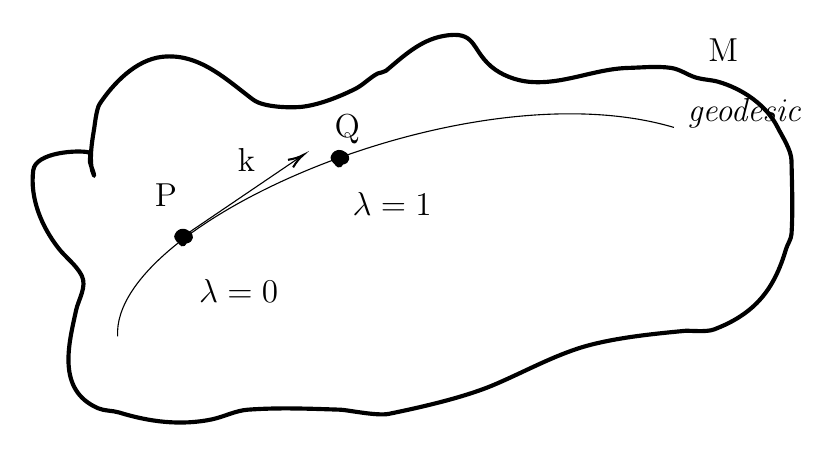
\begin{tikzpicture}[x=0.5pt,y=0.5pt,yscale=-1,xscale=1]
%Shape: Free Drawing [id:dp1885039918119823]
\draw  [line width=1.5] [line join = round][line cap = round] (93,148) .. controls (88.57,139.13) and (91.56,122.99) .. (93,114) .. controls (93.57,110.41) and (94.75,99.38) .. (97,96) .. controls (106.7,81.45) and (122.85,64.21) .. (142,62) .. controls (168.6,58.93) and (188.34,78.26) .. (208,93) .. controls (215.69,98.77) and (236.6,98.96) .. (244,98) .. controls (256.57,96.38) and (271,90.5) .. (282,85) .. controls (287.4,82.3) and (292.6,76.7) .. (298,74) .. controls (300.31,72.84) and (302.08,73.6) .. (304,72) .. controls (316.22,61.81) and (328.41,50.11) .. (345,47) .. controls (369.5,42.41) and (364.91,56.06) .. (380,69) .. controls (387.1,75.09) and (397.7,79.1) .. (407,80) .. controls (431.71,82.39) and (454.53,70.64) .. (479,70) .. controls (489.33,69.73) and (499.77,68.54) .. (510,70) .. controls (516.37,70.91) and (521.84,75.13) .. (528,77) .. controls (532.78,78.45) and (539.06,78.59) .. (544,80) .. controls (561.7,85.06) and (579,97) .. (587,113) .. controls (590.18,119.36) and (596.86,129.28) .. (597,137) .. controls (597.31,154.66) and (598.1,172.37) .. (597,190) .. controls (596.76,193.89) and (594.1,197.26) .. (593,201) .. controls (584.5,229.91) and (570.82,247.64) .. (541,259) .. controls (535.37,261.15) and (523.28,259.68) .. (520,260) .. controls (496.26,262.28) and (465.07,265.31) .. (442,273) .. controls (421.23,279.92) and (402.26,290.4) .. (382,299) .. controls (359.32,308.62) and (326.37,315.81) .. (306,320) .. controls (297.59,321.73) and (276.09,317.17) .. (271,317) .. controls (248.68,316.26) and (226.27,315.32) .. (204,317) .. controls (195.05,317.67) and (186.79,322.19) .. (178,324) .. controls (155.17,328.7) and (132.76,325.7) .. (111,319) .. controls (106.13,317.5) and (100.69,318.01) .. (96,316) .. controls (65.28,302.84) and (74.89,268.85) .. (80,245) .. controls (81.6,237.53) and (88.06,227.88) .. (84,220) .. controls (79.99,212.22) and (72.33,206.94) .. (67,200) .. controls (54.86,184.22) and (46.48,164.14) .. (49,144) .. controls (50.66,130.76) and (81.55,129.25) .. (89,131) .. controls (91.29,131.54) and (89.54,135.69) .. (90,138) .. controls (90.71,141.55) and (93,145.45) .. (93,148) -- cycle ;
%Curve Lines [id:da0957475647721604]
\draw    (110,264) .. controls (105,182) and (364,69) .. (512,113) ;
%Shape: Free Drawing [id:dp8414574325851908]
\draw  [line width=3] [line join = round][line cap = round] (157,196) .. controls (157,194.11) and (151.61,192.72) .. (155,190) .. controls (158.81,186.95) and (165.52,194) .. (158,194) ;
%Shape: Free Drawing [id:dp29626645456634426]
\draw  [line width=3] [line join = round][line cap = round] (270,139) .. controls (270,137.11) and (264.61,135.72) .. (268,133) .. controls (271.81,129.95) and (278.52,137) .. (271,137) ;
%Straight Lines [id:da5664923779397616]
\draw    (157,192) -- (242.34,134.12) ;
\draw [shift={(244,133)}, rotate = 145.86] [color={rgb, 255:red, 0; green, 0; blue, 0 }  ][line width=0.75]    (10.93,-3.29) .. controls (6.95,-1.4) and (3.31,-0.3) .. (0,0) .. controls (3.31,0.3) and (6.95,1.4) .. (10.93,3.29)   ;

% Text Node
\draw (535,47) node [anchor=north west][inner sep=0.75pt]   [align=left] {{\large M}};
% Text Node
\draw (135,152) node [anchor=north west][inner sep=0.75pt]   [align=left] {{\large P}};
% Text Node
\draw (265,102) node [anchor=north west][inner sep=0.75pt]   [align=left] {{\large Q}};
% Text Node
\draw (195,126) node [anchor=north west][inner sep=0.75pt]   [align=left] {{\large k}};
% Text Node
\draw (167,221) node [anchor=north west][inner sep=0.75pt]   [align=left] {\large $\lambda = 0$};
% Text Node
\draw (278,158) node [anchor=north west][inner sep=0.75pt]   [align=left] {\large $\lambda = 1$};
% Text Node
\draw (520,90) node [anchor=north west][inner sep=0.75pt]   [align=left] {\large \emph{geodesic}};
\end{tikzpicture}

\subsection{Riemann Normal Coordinates}
Given a generic $g_{\mu \nu }$ and a point \emph{P}, first I can find vectors $\hat{e}_{\left( \hat{\mu } \right)}$, (where the hat on the \emph{e} means that it is a basis vector and the hat on the index is means that is of inertial coordinates.)\par
Those are requirements to 
\[
g_{\hat{\mu }\hat{\nu }} =  g\left( \hat{e}_{\left( \hat{\mu } \right)}, \hat{e}_{\left( \hat{\nu } \right)} \right) = \eta _{\hat{\mu }\hat{\nu }}
\]
Where the \emph{g( , )} denotes the metric thought as a multilinear map from $T_{P} \times T_{P} \to \mathbb{R}$. This is easy because starting with any set of components for $g_{\mu \nu }$ we can always diagonalize this matrix and rescale the basis vectors to satisfy the above relation.\par
Now we want to find a coordinates system and to do that we will use the exponential map.
Let's define coordinates 
\begin{gather*}
x_{P} = 0 \\
x_{Q} = x^{\hat{\mu }}_{Q} \hat{e}_{\left( \hat{\mu } \right)} = k^{\hat{\mu }} \hat{e}_{\left( \hat{\mu } \right)}
\end{gather*}
where $x^{\hat{\mu }}_{Q}$ is the inverse of \emph{exp\textsubscript{P}}, \emph{x\textsubscript{Q}} is the position vector and it is represented as a linear combination of basis vectors.\par
So, RNC are $x_{Q } = k^{\mu } \hat{e}_{\left( \hat{\mu } \right)}$, and a particular property is that in this coordinates system 
\[
x^{\hat{\mu }}\left( \lambda  \right) = \lambda k^{\hat{\mu }}
\]
is a geodesic, only in these coordinates.
\subsubsection{More in deep explanation}
Now, I understand that if this is the first time approaching this it's kinda difficult to get the point. 
The part that makes the exponential map useful is that it's hard to find a coordinates system $x^{\hat{\mu }}$ for which the basis vectors $\{ \hat{e}_{\left( h\mu  \right)}\}$ are made of $\hat{e}_{\left( \hat{\mu } \right)} = \partial_{\hat{\mu } }$m and such that the first partial derivatives of $g_{\hat{\mu }\hat{\nu }}$ vanish. But the exponential map achieves that automatically. For any point \emph{Q} sufficiently close to \emph{P}, there is a unique geodesic path connecting \emph{P} to \emph{Q}, and a unique parametrization $\lambda $. At \emph{P} the tangent vector can be written as a linear combination of our basis vectors $k = k^{\hat{\mu }} \hat{e}_{\left( \hat{\mu } \right)}$. Then we define $x^{\hat{\mu }}$ to be these components $x^{\hat{\mu }}\left( Q \right) = k^{\hat{\mu }}$

\subsubsection{Check on RNC}
We want to verify that RNC satisfy $\partial_{\hat{\rho }} g_{\hat{\mu }\hat{\nu }}\left( P \right) = 0$. Noting that a ray  in the tangent space gets mapped to a geodesic by the exponential map, leads to see that in RNC a curve $x^{\hat{\mu }}\left( \lambda  \right)$ of the form
\[
x^{\hat{\mu }} \left( \lambda  \right) = \lambda k^{\hat{\mu }}
\]
will solve the geodesic equation.  Plugging this inside gives
\begin{equation}
\frac{d ^{2} x^{\hat{\mu }}}{d \lambda ^{2}} + \Gamma ^{\hat{\mu }}_{\hat{\alpha }\hat{\beta }} \frac{d x^{\hat{\alpha }}}{d \lambda }\frac{d x^{\hat{\beta }}}{d \lambda } = 0
\end{equation}
where the second derivative is null, and the other two partial derivatives correspond to $k^{\hat{\alpha }}, k^{\hat{\beta }}$. So we are left with
\begin{equation}
\Gamma ^{\hat{\mu }}_{\hat{\alpha }\hat{\beta }} k^{\hat{\alpha }}k^{\hat{\beta }} = 0, \forall k
\end{equation}
and since it true for every \emph{k}
\[
\Gamma ^{\hat{\mu }}_{\hat{\alpha }\hat{\beta }} \left( P \right) = 0
\]
Now we apply the metric compatibility
\begin{equation}
\nabla _{\hat{\rho }} \left( g_{\hat{\mu }\hat{\nu }} \right) = \partial_{\hat{\rho }} g_{\hat{\mu }\hat{\nu }} - \Gamma - \Gamma 
\end{equation}
And each term is equal to zero. RNCs makes the LICs.

\subsection{Riemann Curvature Tensor}

As we already discussed, parallel transport of a vector around a closed loop in a curved space will result in a different vector than the one we started with. The transformation depends on the total curvature enclosed by the loop. \par
Since spacetime looks flat locally, if we define a loop made by two infinitesimal vectors $A^{\mu }$ and $B^{\nu }$ we can  perform parallel transport on a vector $V^{\mu }$ by moving it anti-clockwise.


\tikzset{every picture/.style={line width=0.5pt}} %set default line width to 0.75pt      
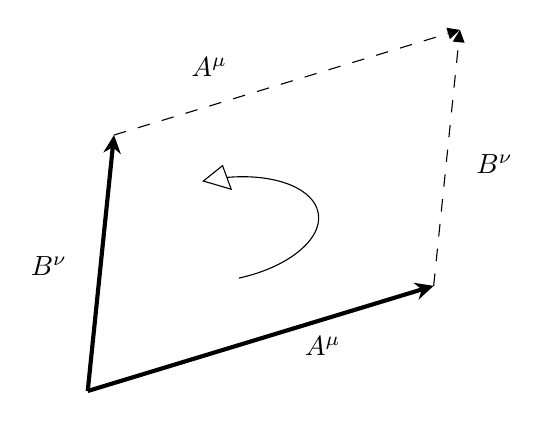
\begin{tikzpicture}[x=0.5pt,y=0.5pt,yscale=-1,xscale=1]
%uncomment if require: \path (0,300); %set diagram left start at 0, and has height of 300

%Straight Lines [id:da4139814907991093] 
\draw [line width=1.5]    (215,277) -- (461.17,202.16) ;
\draw [shift={(465,201)}, rotate = 163.09] [fill={rgb, 255:red, 0; green, 0; blue, 0 }  ][line width=0.08]  [draw opacity=0] (13.4,-6.43) -- (0,0) -- (13.4,6.44) -- (8.9,0) -- cycle    ;
%Straight Lines [id:da37994344236993594] 
\draw [line width=1.5]    (215,277) -- (233.59,95.98) ;
\draw [shift={(234,92)}, rotate = 95.86] [fill={rgb, 255:red, 0; green, 0; blue, 0 }  ][line width=0.08]  [draw opacity=0] (13.4,-6.43) -- (0,0) -- (13.4,6.44) -- (8.9,0) -- cycle    ;
%Straight Lines [id:da11748394321022726] 
\draw  [dash pattern={on 4.5pt off 4.5pt}]  (465,201) -- (483.69,18.98) ;
\draw [shift={(484,16)}, rotate = 95.86] [fill={rgb, 255:red, 0; green, 0; blue, 0 }  ][line width=0.08]  [draw opacity=0] (8.93,-4.29) -- (0,0) -- (8.93,4.29) -- cycle    ;
%Straight Lines [id:da04954610847070795] 
\draw  [dash pattern={on 4.5pt off 4.5pt}]  (234,92) -- (481.13,16.87) ;
\draw [shift={(484,16)}, rotate = 163.09] [fill={rgb, 255:red, 0; green, 0; blue, 0 }  ][line width=0.08]  [draw opacity=0] (8.93,-4.29) -- (0,0) -- (8.93,4.29) -- cycle    ;
%Curve Right Arrow [id:dp34474738978659925] 
\draw  [fill={rgb, 255:red, 255; green, 255; blue, 255 }  ,fill opacity=1 ] (380.74,145.2) .. controls (387.81,164.58) and (362.48,187.06) .. (324.16,195.41) -- (324.16,195.41) .. controls (362.48,187.06) and (387.81,164.58) .. (380.74,145.2) -- cycle ;\draw  [fill={rgb, 255:red, 255; green, 255; blue, 255 }  ,fill opacity=1 ] (380.74,145.2) .. controls (374.73,128.72) and (347.22,119.8) .. (315.56,122.64) -- (318.67,131.17) -- (298.58,125.25) -- (312.44,114.11) -- (315.56,122.64) .. controls (347.22,119.8) and (374.73,128.72) .. (380.74,145.2) -- cycle ;

% Text Node
\draw (172,178) node [anchor=north west][inner sep=0.75pt]   [align=left] { $B^{\nu }$ };
% Text Node
\draw (370,236) node [anchor=north west][inner sep=0.75pt]   [align=left] { $A^{\mu }$};
% Text Node
\draw (494,104) node [anchor=north west][inner sep=0.75pt]   [align=left] { $B^{\nu }$};
% Text Node
\draw (288,34) node [anchor=north west][inner sep=0.75pt]   [align=left] { $A^{\mu }$};
\end{tikzpicture}
\bigskip

As we know the action of parallel transport is independent on the coordinates, so there should be a tensor that quantifies the change of the vector, so with an upper and a lower index. Depending also on vectors \textbf{A} and \textbf{B}, there are two additional lower indices. And this tensor must be anti-symmetric since we can walk the loop in the opposite direction, and the outcome would be the inverse. So we should get something like this
\begin{equation}
\delta V^{\mu } = R^{\mu }_{\alpha \beta \gamma }A^{\alpha }B^{\beta }V^{\gamma}
\end{equation}
As decided above this tensor should be anti-symmetric on the \emph{last two indices}.
\[
R^{\mu }_{\alpha \beta \gamma } = - R^{\mu }_{\alpha \gamma  \beta }
\]
To compute what's inside the \textbf{R} tensor is kinda difficult so we take a related operation, the commutator of two covariant derivatives. \par
The relation between the two is because the covariant derivative of a tensor in a certain direction measures how much the tensor changes relative to what it would have been if it had been parallel transported, because the covariant derivative of a tensor in a direction along which is parallel transported is null. The commutator of two covariant derivatives measures the difference between parallel transporting the tensor first one way and then the other, and viceversa.\bigskip


\tikzset{every picture/.style={line width=0.5pt}} %set default line width to 0.75pt       
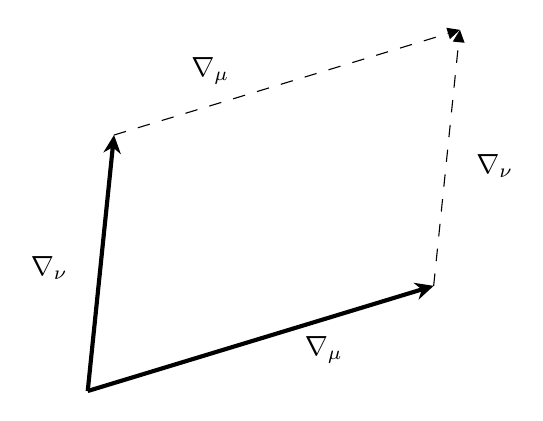
\begin{tikzpicture}[x=0.5pt,y=0.5pt,yscale=-1,xscale=1]
%uncomment if require: \path (0,300); %set diagram left start at 0, and has height of 300

%Straight Lines [id:da4139814907991093] 
\draw [line width=1.5]    (215,277) -- (461.17,202.16) ;
\draw [shift={(465,201)}, rotate = 163.09] [fill={rgb, 255:red, 0; green, 0; blue, 0 }  ][line width=0.08]  [draw opacity=0] (13.4,-6.43) -- (0,0) -- (13.4,6.44) -- (8.9,0) -- cycle    ;
%Straight Lines [id:da37994344236993594] 
\draw [line width=1.5]    (215,277) -- (233.59,95.98) ;
\draw [shift={(234,92)}, rotate = 95.86] [fill={rgb, 255:red, 0; green, 0; blue, 0 }  ][line width=0.08]  [draw opacity=0] (13.4,-6.43) -- (0,0) -- (13.4,6.44) -- (8.9,0) -- cycle    ;
%Straight Lines [id:da11748394321022726] 
\draw  [dash pattern={on 4.5pt off 4.5pt}]  (465,201) -- (483.69,18.98) ;
\draw [shift={(484,16)}, rotate = 95.86] [fill={rgb, 255:red, 0; green, 0; blue, 0 }  ][line width=0.08]  [draw opacity=0] (8.93,-4.29) -- (0,0) -- (8.93,4.29) -- cycle    ;
%Straight Lines [id:da04954610847070795] 
\draw  [dash pattern={on 4.5pt off 4.5pt}]  (234,92) -- (481.13,16.87) ;
\draw [shift={(484,16)}, rotate = 163.09] [fill={rgb, 255:red, 0; green, 0; blue, 0 }  ][line width=0.08]  [draw opacity=0] (8.93,-4.29) -- (0,0) -- (8.93,4.29) -- cycle    ;

% Text Node
\draw (172,178) node [anchor=north west][inner sep=0.75pt]   [align=left] { $\nabla _{\nu }$};
% Text Node
\draw (370,236) node [anchor=north west][inner sep=0.75pt]   [align=left] { $\nabla _{\mu }$};
% Text Node
\draw (494,104) node [anchor=north west][inner sep=0.75pt]   [align=left] { $\nabla _{\nu }$};
% Text Node
\draw (288,34) node [anchor=north west][inner sep=0.75pt]   [align=left] { $\nabla _{\mu }$};
\end{tikzpicture}
\bigskip

We could do the computation with a scalar but
\begin{equation}
	[\nabla _{\mu }, \nabla _{\nu }] \phi = \nabla _{\mu}\left( \nabla _{\nu }\phi  \right) -\nabla _{\nu }\left( \nabla _{\mu }\phi  \right) = \partial_{\mu }\left( \partial_{\nu }\phi  \right) - \partial_{\nu }\left( \partial_{\mu }\phi  \right) = 0
\end{equation}
Not only is equal to zero, but it's trivially zero.\par
So we will use a vector
\begin{gather*}
	[\nabla _{\mu },\nabla _{\nu }] V^{\rho } = \nabla _{\mu }\left( \nabla _{\nu }V^{\rho } \right) - \nabla_{\nu }\left( \nabla _{\mu }V^{\rho } \right)	 \\
	\text{ now we take just one of the terms } \\
	\nabla _{\mu }\left( \nabla _{\nu } V^{\rho } \right) = \partial_{\mu } \left( \nabla _{\nu } V^{\rho } \right) + \Gamma ^{\rho }_{\mu \beta } \nabla _{\nu }V^{\beta } - \Gamma ^{\beta }_{\mu \nu } \nabla _{\beta } V^{\rho } \\
	\text{ again, we take the first term of the second part } \\
	\partial_{\mu }\left( \partial_{\nu }V^{\rho } + \Gamma ^{\rho }_{\nu \alpha } V^{\alpha } \right) + \Gamma ^{\rho }_{\mu \beta } \left( \partial_{\nu }V^{\beta } + \Gamma ^{\beta}_{\nu \alpha } V^{\alpha } \right) - \Gamma ^{\beta }_{\mu \nu } \nabla _{\beta }V^{\rho } \\
	\partial_{\mu }\partial_{\nu }V^{\rho } + \left( \partial_{\mu } \Gamma ^{\rho }_{\nu \alpha } \right)V^{\alpha } + \Gamma ^{\rho }_{\nu \alpha } \partial_{\mu }V^{\alpha } + \Gamma ^{\rho }_{\mu \beta } \partial_{\nu }V^{\beta } + \Gamma ^{\rho }_{\mu \beta }\Gamma ^{\beta }_{\nu \alpha } V^{\alpha }- \Gamma ^{\beta }_{\mu \nu }\nabla _{\beta} V^{\rho }
\end{gather*}
Now, let's look at this last row for some simplifications.
\begin{itemize}
\item The first term is symmetric in $\mu , \nu $.
\item The sum of the third and the fourth is symmetric in $\mu , \nu $ if we swap the dummy index $\beta \to \alpha $.
\item The last term is symmetric but only with \emph{zero torsion,}
\end{itemize}
The terms that are symmetric vanish since we are using the operator of anti-symmetry. So we are left, with
\begin{gather}
	[\nabla _{\mu }, \nabla _{\nu }]V^{\rho } =\\
	= \left( \partial_{\mu }\Gamma ^{\rho }_{\nu \alpha } - \partial_{\nu }\Gamma ^{\rho }_{\mu \alpha } \right)V^{\alpha } + \left( \Gamma ^{\rho }_{\mu \beta } \Gamma ^{\beta }_{\nu \alpha } - \Gamma ^{\rho }_{\nu \beta }\Gamma ^{\beta }_{\mu \alpha } \right)V^{\alpha } - \left( \Gamma ^{\beta }_{\mu \nu } - \Gamma ^{\beta }_{\nu \mu } \right)\nabla _{\beta }V^{\rho }
\end{gather}
This last piece has equivalent to the \emph{torsion} that is
\[
T^{\beta }_{\mu \nu }\nabla _{\beta }V^{\rho }
\]
but since we work with torsion free connections, it's zero. We are left with
\begin{equation}
	[\nabla _{\mu }, \nabla _{\nu }]V^{\rho } = [\partial_{\mu }\Gamma ^{\rho }_{\nu \alpha } - \partial_{\nu }\Gamma ^{\rho }_{\mu \alpha } + \Gamma  ^{\rho }_{\mu  \beta }\Gamma  ^{ \beta }_{\nu  \alpha } - \Gamma ^{\rho }_{\nu \beta }\Gamma ^{\beta }_{\mu \alpha }] V^{\alpha }
\end{equation}
And this, can be written as 
\begin{equation}
	[\nabla _{\mu }, \nabla _{\nu }] V^{ \rho } = R^{\rho }_{\sigma \mu \nu } V^{\sigma }
\end{equation}
that is the Riemann Tensor.







\section{Lec 14}
Today we will talk about some properties of the Riemann tensor.\par
\[
	[\nabla _{\mu }, \nabla _{\nu }] V^{\rho } = R^{\rho }_{\sigma \mu \nu } V^{\sigma } + \text{ torsion, ( } \nabla _{\rho }V^{\sigma }\text{)}
\]
and 
\[
	R^{\rho }_{\sigma \mu \nu } = \partial_{\mu }\Gamma^{\rho }_{\nu \sigma } - \partial_{\nu }\Gamma ^{\rho }_{\mu \sigma } + \Gamma  ^{\rho }_{\mu \lambda } \Gamma ^{\lambda }_{\nu \sigma } -\Gamma ^{\rho }_{\nu \lambda }\Gamma ^{\lambda }_{\mu \sigma }
\]
The simplest way to derive the symmetries is to examine the Riemann tensor with all lower indices.
\[
R_{\rho \sigma \mu \nu } = g_{\rho \lambda } R^{\lambda }_{\sigma \mu \nu }
\]
There are four properties that can help us reduce the number of independent entries of this tensor from a number of $n^{4}$ to just 20 (in 4 dimensions spaces).
\begin{enumerate}
\item $R_{\rho \sigma \mu \nu } = - R_{\rho \sigma \nu \mu } $ 
\item ... 
	\item ...
	\item ...
\end{enumerate}
So the Riemann tensor is anti-symmetric on the last two indices.\par
We now consider the components of this tensor in locally inertial coordinates $x^{\hat{\mu }}$ at some point \emph{P}. Then the Christoffel symbols will vanish, but not their derivatives.
\begin{equation}
\begin{cases}
g_{\hat{\mu }\hat{\nu }} \left( P \right) = \eta _{\hat{\mu }\hat{\nu }} \\
\partial_{\hat{\rho }} g_{\hat{\mu }\hat{\nu }}\left( P \right) = 0 \to \Gamma ^{\hat{\alpha }}_{\hat{\mu }\hat{\nu }} \left( P \right) = 0 \\
\end{cases}
\end{equation}
We are left with
\begin{gather*}
R_{\hat{\rho }\hat{\sigma }\hat{\mu }\hat{\nu }} \left( P \right) = g_{\hat{\rho }\hat{\lambda }} \left( \partial_{\hat{\mu }} \Gamma ^{\hat{\lambda }}_{\hat{\nu }\hat{\sigma }} - \partial_{\hat{\nu }} \Gamma ^{\hat{\lambda }}_{\hat{\mu }\hat{\sigma }} \right)  = \\
= g_{\hat{\rho }\hat{\lambda }} \frac{1}{2} \partial_{\hat{\mu } } [ g^{\hat{\lambda }\hat{\alpha }} \left( \partial_{\hat{\nu }} g_{\hat{\alpha  }\hat{\sigma }} + \partial_{\hat{\sigma }} g_{\hat{\alpha }\hat{\nu }} - \partial_{\hat{\alpha }} g_{\hat{\sigma }\hat{\nu }} \right) ] - \left( \hat{\mu } \leftrightarrow \hat{\nu } \right) \\
= \frac{g_{\hat{\rho }\hat{\lambda }}}{2} g^{\hat{\lambda }\hat{\alpha }} [ \partial_{\hat{\mu }} \partial_{\hat{\nu }} g_{\hat{\alpha }\hat{\sigma }} + \partial_{\hat{\mu }}\partial_{\hat{\sigma }} g_{\hat{\alpha }\hat{\nu }} - \partial_{\hat{\mu }}\partial_{\hat{\alpha }} g_{\hat{\sigma }\hat{\nu }}] - \left( \hat{\mu } \leftrightarrow \hat{\nu } \right)
\end{gather*} 
Now as usual let's look for some simplifications: \par
The first term inside the square brackets is symmetric so it goes away. The product of $g_{\hat{\rho }\hat{\lambda }} g^{\hat{\lambda }\hat{\alpha }} = \delta ^{\hat{\alpha }}_{\hat{\rho }} $ so every $\alpha $ becomes a $\rho $. We are left with
\begin{equation}
	R_{\hat{\rho }\hat{\sigma }\hat{\mu }\hat{\nu }} = \frac{1}{2} [\partial_{\hat{\mu }}\partial_{\hat{\sigma }} g_{\hat{\rho }\hat{\nu }} - \partial_{\hat{\mu }}\partial_{\hat{\rho }}g_{\hat{\sigma }\hat{\nu }} - \partial_{\hat{\nu }}\partial_{\hat{\sigma }} g_{\hat{\rho }\hat{\mu }}+ \partial_{\hat{\nu }}\partial_{\hat{\rho }}g_{\hat{\sigma }\hat{\mu }}]
\end{equation}
By looking at it, we see that the tensor is antisymmetric on it's first two indices
\[
R_{\rho \sigma \mu \nu } = - R_{\sigma \rho \mu \nu }
\]
also for exercise one can see that exchanging block, the tensor is invariant under interchange of the first pair of indices with the second:
\[
R_{\rho \sigma \mu \nu } = R_{\mu \nu \rho \sigma }
\]
another thing that could be checked is that the complete anti-symmetrization of this tensor is null
\[
	R_{[\rho \sigma \mu \nu ]} = 0
\]
so the properties are
\begin{enumerate}
\item $R_{\rho \sigma \mu \nu }  = - R_{\rho \sigma \nu \mu }$
\item $R_{\rho \sigma \mu \nu } = - R_{\sigma \rho \mu \nu }$
\item $R_{\rho \sigma \mu \nu } = R_{\mu \nu \rho \sigma }$
\item $R_{[\rho \sigma \mu \nu ]} = 0$
\end{enumerate}
Now we have to count how many independent entries we are left with.\par
Starting from anti-symmetry on the first two and last two indices and symmetry on the exchange of this pairs, we can think of a symmetric matrix $R_{[\rho \sigma ][\mu \nu ]}$. The pairs are thought as individual indices. An $m\times m$ symmetric matrix has 
\[
\frac{m\left( m+1 \right)}{2}
\]
individual components, while the two anti-symmetric matrices have
\[
\frac{n\left( n-1 \right)}{2}
\]
free components, so
\[
	\frac{1}{2} \left[ \frac{1}{2} n\left( n-1 \right)\right] \left[ \frac{1}{2} n \left( n-1 \right)+1\right] = \frac{1}{8} \left( n^{4} -2n^{3} +3n^{2} -2n \right)
\]
Independent components, and putting $n=4$ we get 21 independent entries. \par
But.\par
We know that a totally antisymmetric tensor with 4 indices has
\[
\frac{n\left( n-1 \right)\left( n-2 \right)\left( n-3 \right)}{4!}
\]
terms and it helps reducing the number of independent components by 1.\par
So, in conclusion the Riemann tensor has 20 free components.\par
\subsubsection{Bianchi Identity}
It's a relation that tells us about the covariant derivative of the Riemann tensor.
There is an algebraic version of the Bianchi Identity that is expressed as
\begin{equation}
R^{\rho }_{\sigma \mu \nu } + R^{\rho }_{\nu \sigma \mu } + R^{\rho }_{\mu \nu \sigma } = 0
\end{equation}
that states that the cyclic permutation of the lower three indices sum to zero.\par
There is a differential way to define the Bianchi Identity that is
\begin{equation}
	\nabla_{[\lambda }R_{\mu \nu ]\rho \sigma } = 0		
\end{equation}

\subsubsection{Ricci tensor}
It is defined as
\begin{equation}
R_{\mu \nu } = R^{\lambda }_{\mu \lambda \nu }
\end{equation}
Is it symmetric? Yes.
\[
R_{\nu \mu } = R^{\lambda }_{ \nu \lambda \mu } = g^{\rho \lambda }R_{\rho \nu \lambda \mu } = g^{\rho \lambda }R_{\lambda \mu \rho \nu } = R^{\lambda }_{\mu \lambda \nu } = R_{\mu \nu }
\]
The trace of the Ricci tensor is the Ricci scalar
\begin{equation}
R = g^{\mu \nu }R_{\mu \nu }
\end{equation}

\subsection{A kind of Einstein Equation}
Professor gave us this equation, that is an arrival point
\begin{equation}
R_{\mu \nu } - \frac{1}{2}g_{\mu \nu }R = 8\pi G T_{\mu \nu }
\end{equation}
as we know $T_{\mu \nu }$ describe energy and momentum. We don't want to give up conservation of energy and momentum. 
We know in flat spacetime that
\[
\partial_{\mu }T_{\mu \nu } = 0 
\]
and so in curved spacetime 
\[
\nabla _{\mu }T^{\mu \nu }= 0
\]
Now we need a tensor in order to keep it null when we change frame. This means that also in the EE we need 
\[
\nabla _{\mu }\left( G_{\mu \nu } \right) = 0
\]
where the tensor $G_{\mu \nu }$ called Einstein tensor is defined as
\begin{equation}
g_{\mu \nu } = R_{\mu \nu } - \frac{1}{2} g_{\mu \nu }R
\end{equation}
let's prove this.
\begin{gather*}
	g^{\mu \lambda } g^{\nu \sigma } \left[ \nabla _{\lambda } R_{\rho \sigma \mu \nu } + \nabla _{\rho }R_{\sigma \lambda \mu \nu } + \nabla _{\sigma }R_{\lambda \rho \mu \nu }\right] = 0 \\
	\nabla ^{\mu }R_{\rho \mu } - \nabla _{\rho }R + \nabla ^{\mu }R_{\rho \nu }  = 0\\
	\text{ or } \nabla ^{\mu }R_{\rho \mu } = \frac{1}{2} \nabla _{\rho }R
\end{gather*}


































\section{Lec 15}

\subsection{Einstein Equation}
Today we will derive the Einstein Equation. We will use a technique called \emph{minimal coupling principle}. It has three steps
\begin{enumerate}
\item Take a physics law valid in flat spacetime (e.g. poisson equation for gravitational potential).
\item write it in a coordinates independent form ( tensorial).
\item Assume it is valid for curved spacetime.
\end{enumerate}

Let's start with the first step. \par
We consider the motion of freely-falling particles. From cartesian coordinates, $x^{\mu }$, we have a straigt line \[
\frac{d ^{2}x^{\mu }}{d \lambda ^{2}} = 0 
\]
n.b. this is not a tensorial relation: $\frac{d x^{\mu }}{d \lambda }$ is a well-defined vector, but the second derivative is not.
Now I change coordinates, but keeping spacetime flat. This is because a law that changes with coordinates is not coordinates independent.
\[
\frac{d }{d \lambda }\left( \frac{d x^{\mu }}{d \lambda } \right) = 0
\]
this one is composed by a vector inside the brackets, while the operator outside is not a tensor. \par
We could use the chain rule to write
\[
\frac{d ^{2}x^{\mu }}{d \lambda ^{2}} = \frac{d x^{\sigma }}{d \lambda }\partial_{\sigma }\frac{d x^{\mu }}{d \lambda }
\]
but the partial derivative is still a problem. Maybe we should use the covariant one.
So we get
\[
	\frac{d x^{\sigma }}{d \lambda }\nabla _{\sigma } \left( \frac{d x^{\mu }}{d \lambda } \right) = \frac{d x^{\sigma }}{d \lambda }\left[ \partial_{\sigma } \left( \frac{d x^{\mu }}{d \lambda } \right) + \Gamma ^{\mu }_{\sigma \alpha } \frac{d x^{\alpha }}{d \lambda }\right] = 0
\]
in the end
\[
\frac{d ^{2}x^{\mu }}{d \lambda ^{2}} + \Gamma ^{\mu }_{\sigma \alpha }\frac{d x^{\sigma }}{d \lambda }\frac{d x^{\alpha }}{d \lambda } = 0
\]
This is the geodesic equation. In general relativity we said freely-falling particles move along geodesics. Now we have generalized a small thing to curved spacetime but it is different from saying that this describes gravity.\par
So, let's show how results from the Newtonian limit fit in this picture. This limit has three requirements
\begin{itemize}
\item slowly moving particles $v \ll c$
\item weak gravitational field, so the metric could be Minkowskian with a little perturbation
	\[
		g_{\mu \nu } = \eta _{\mu \nu } + h_{\mu \nu }, |h_{\mu \nu }|\ll 1
	\]
\item the gravitational field is also static, it does not change in time ( $\partial_{0}g_{\mu \nu } = 0$)
\end{itemize}
We consider time-like geodesics, so trajectories of massive particles, so it is useful to parametrize them using the proper time $\tau $.
\[
\frac{d ^{2}x^{\mu }}{d \tau ^{2}} + \Gamma ^{\mu }_{\alpha  \beta } \frac{d x^{\alpha }}{d \tau }\frac{d x^{\beta }}{d \tau } = 0
\]
I want to use this to describe the motion under gravitational field, so we want to recover the $\vec{a} = -\vec{\nabla } \phi $. $\phi $ is hidden inside the connection, while $\vec{a}$ is the second derivative. \par
Since we required slow motion 
\[
\frac{d t}{d \tau } \gg \frac{d x^{i}}{d \tau }	
\]
So the geodesics equation becomes
\begin{equation}
\frac{d ^{2}x^{\mu }}{d \tau ^{2}} + \Gamma ^{\mu }_{00}\frac{d x^{0}}{d \tau }\frac{d x^{0}}{d \tau } = 0 \to  \frac{d ^{2}x^{\mu }}{d \tau ^{2}} + \Gamma ^{\mu }_{00}\left( \frac{d t}{d \tau } \right)^{2} = 0
\end{equation}
In this situation I just need 4 entries for the connection, that is defined as
\[
	\Gamma ^{\rho }_{\mu \nu } = \frac{1}{2} g^{\rho \sigma }\left[ \partial_{\mu } g_{\sigma\nu } + \partial_{\nu }g_{\sigma \mu } - \partial_{\sigma }g_{\mu \nu } \right]
\]
so
\begin{equation}
	\Gamma ^{\mu }_{00} = \frac{1}{2} g^{\mu \alpha } \left[ \partial_{0}g_{\alpha 0} + \partial_{0}g_{\alpha 0} - \partial_{\alpha }g_{00} \right]
\end{equation}
since the condition of a static gravitational field, the time derivatives are equal to zero. We are left with 
\[
\partial_{\alpha }g_{00} = \partial_{\alpha }\left( \eta _{00} + h_{00} \right) = \partial_{\alpha }h_{00}
\]
because the Minkowskian metric tensor is constant. 
\begin{equation}
\Gamma ^{\mu }_{00} = -\frac{1}{2} g^{\mu \alpha } \partial_{\alpha }h_{00} = 
\end{equation}























\chapter{Black Holes}
\section{Lec 16}
\subsection{Scharzschild's Metric}
The most obvious application of a theory of gravity is the case of spherical symmetry, that is like the one of the Earth or the Sun. We will start with a solution of the vacuum outside them, because is both easier and more useful. 
A specific solution of the Einstein Equation is the Schwarzschild Solution, for a static (components of $g_{\mu \nu }$ do not depend on time) spacetime with $\left( S^{2} \right)$ symmetry.\par
There is more than one way to derive this solution, we will use the most boring one:
\begin{enumerate}
\item \emph{Guess} a generic form for $g_{\mu \nu } $
\item Compute $\Gamma ^{\mu }_{\alpha \beta }$, $R^{\alpha }_{\beta \gamma \delta }$, $R_{\alpha \beta }$
\item Solve $R_{\mu \nu } = 0$, since the space outside the sun is empty space, vacuum.
\end{enumerate}

Let's start from the \textbf{guess} step.
We want to \emph{guess} the metric in spherical coordinates 
\begin{equation}\label{eq:polarmetric}
ds^{2}= -A\left( r \right) dt^{2} + B\left( r \right) dr^{2} + C\left( r \right) r^{2}d\Omega ^{2}
\end{equation}

where $d\Omega ^{2}$ is the metric on a $S^{2}$ sphere.
\[
	d\Omega ^{2} = d\theta ^{2} + sin^{2}\theta d\phi ^{2}
\]
Since we are almost in the vacuum, we can start in fact from the Minkowski metric in polar coordinates: $ds^{2 }=-dt^{2} +dr^{2}+r^{2}d\Omega ^{2} $.
Now we would like simplify a little eq.\ref{eq:polarmetric}:
\begin{itemize}
\item $r^{2}C\left( r \right) \to  r^{2}$, this is a change of coordinates, nothing to do with spherical symmetry, but know we have to rescale $A\left( r \right), B\left( r \right)$
\item $A \equiv e^{2\alpha \left( r \right)}$
\item $B\equiv e^{2\beta \left( r \right)}$
\end{itemize}.
With this, the most general guess is:
\begin{equation}\label{eq:pmetric2}
ds^{2} = -e^{2\alpha \left( r \right)}dt^{2} + e^{2\beta \left( r \right)}dr^{2} + r^{2}d\Omega ^{2}
\end{equation}
We have now two unknown functions $\alpha ,\beta $ of the radial coordinate, not time because of staticness, not angle because of isotropy.\par
Now it's time to \textbf{compute the metric tensor, Christoffel thing and Riemann tensor.}\par
\paragraph{Metric} 
\begin{equation}
\begin{matrix} 
g_{tt}= -e^{2\alpha \left( r \right)} & g_{rr}=e^{2\beta \left( r \right)} & g_{\theta \theta }= r^{2} & g_{\phi \phi } = r^{2}sin^{2}\theta  \\
g^{tt}=-e^{-2\alpha \left( r \right)} & g^{rr}=e^{-2\beta \left( r \right)} & g^{\theta \theta }= \frac{1}{r^{2}} & g^{\phi \phi }=\frac{1}{r^{2}sin^{2}\theta } \\
\end{matrix}
\end{equation}
other entries are null.
\paragraph{Christoffel Symbols}
 In most generic spacetimes there are 40 independent Christoffel coefficients. %unclear why there are less
As you may remember the Christoffel connection is defined as
\begin{equation}
	\Gamma ^{\rho }_{\mu \nu } = \frac{1}{2}g^{\rho \sigma }\left[ \partial_{\mu }g_{\sigma \nu }+\partial_{\nu }g_{\sigma \mu }-\partial_{\sigma }g_{\mu \nu }\right]
\end{equation}
if $\rho = t $:
\begin{equation}
	\Gamma^{t}_{\mu \nu } = \frac{1}{2} g^{t\sigma } \left[ \partial_{\mu }g_{\sigma \nu }+\partial_{\nu }g_{\sigma \mu }- \partial_{\sigma }g_{\mu \nu }\right]
\end{equation}
from this I get contribution only for $\sigma =t$, because of how is defined the metric. 
\begin{equation}
	\left( \sigma = t \right) \to \Gamma ^{t}_{\mu \nu } = \frac{1}{2}g^{tt}\left[ \partial_{\mu }g_{t\nu } + \partial_{\nu }g_{t\mu } - \partial_{t}g_{\mu \nu }\right]
\end{equation}
At this point, one immediately see that the last derivative is null since staticness.\par
If $\mu , \nu \neq t \to 0$ since components of the metric tensor with mixed indices are null. 
\begin{equation}
\Gamma ^{t}_{tr} = \frac{1}{2} g^{tt}\partial_{r}g_{tt} = \frac{1}{2} \left( -e^{-2\alpha }\left( r \right) \right)\left( -2\alpha ' e^{+2\alpha \left( r \right)} \right) = \alpha ' \to \Gamma ^{t}_{tr} = \alpha '
\end{equation}
Now for $\rho =r$, so $\sigma $ must be \emph{r}, too:
\begin{equation}
	\Gamma ^{t}_{\mu \nu } = \frac{1}{2} g^{rr}\left[ \partial_{\mu }g_{r\nu }+ \partial_{\nu }g_{r\mu }-\partial_{r}g_{\mu \nu }\right]
\end{equation}
if  also$\mu ,\nu  = r$
\begin{equation}
	\Gamma ^{r}_{rr} = \frac{1}{2} g^{rr}\left[ \partial_{r}g_{rr}+\partial_{r}g_{rr}-\partial_{r}g_{rr}\right] = \frac{1}{2}g^{rr}d_{r}g_{rr} = \beta ' \to  \Gamma ^{r}_{rr} = \beta '
\end{equation}
instead, if $\mu ,\nu  = t$:
\begin{equation}
\Gamma^{r}_{tt} = \frac{1}{2}g^{rr} \left( \partial_{t}g_{rt} +\partial_{t}g_{rt}-\partial_{r}g_{tt} \right) = -\frac{1}{2} g^{rr}\partial_{r}g_{tt} = \frac{1}{2}e^{-2\beta }e^{2\alpha }2\alpha ' = \alpha ' e^{2\left( \alpha -\beta  \right)}
\end{equation}
The remaining components are given but it would be interesting retrieving them by yourself, since professor said that he could ask to compute one component of the $\Gamma $ at the exam.
\begin{equation}
\begin{matrix}
\Gamma ^{r}_{\theta \theta } = - r e^{-2\beta } & \Gamma ^{r}_{\phi \phi } = -r sin^{2}\theta e^{-2\beta } & \Gamma^{\theta }_{r\theta } = \frac{1}{r} \\
\Gamma ^{\theta }_{\phi \phi } = -sin \theta cos \theta  & \Gamma ^{\phi }_{r\phi } = \frac{1}{r} & \Gamma ^{\phi }_{\theta \phi } = \frac{cos \theta }{sin \theta } ,
\end{matrix} 
\end{equation}

\paragraph{Riemann tensor}
As we know it is defined as
\[
R^{\rho }_{\sigma \mu \nu } = \partial_{\mu }\Gamma ^{\rho }_{\nu \sigma }- \partial_{\nu }\Gamma ^{\rho }_{\mu \sigma } + \Gamma ^{\rho }_{\mu \lambda }\Gamma ^{\lambda }_{\nu \sigma }- \Gamma ^{\rho }_{\nu \lambda }\Gamma ^{\lambda }_{\mu \sigma }
\]
And since we know all the $\Gamma$s we should know every Riemann tensor component. Eventually we care about $R_{\mu \nu } = 0$, so we will impose
\[
R_{\alpha \alpha } = 0, \alpha \text{ fixed } \to R^{\beta }_{\alpha \beta \alpha }
\]
\begin{itemize}
\item $R^{t}_{rtr} = -\alpha^{\prime \prime } -\alpha ^{\prime 2} +\alpha^{\prime }\beta ^{\prime }$
\item $R^{t}_{\theta  t \theta } = -r \alpha^{\prime } e^{-2\beta }$
\item $R^{t}_{\phi t \phi } = -r \alpha^{\prime } sin^{2} \theta  e^{-2\beta }$
\item $R^{r}_{\theta r \theta } = r\beta ' e^{-2\beta }$
\item $R^{r}_{\phi r \phi } = r \beta ' sin^{2}\theta  e^{-2\beta }$
\item $R^{\theta }_{\phi \theta \phi } = \left( 1-e^{-2\beta } \right)sin^{2} \theta $
\end{itemize}
How to compute the others?
\begin{equation}
R^{r}_{trt} = g^{rr}R_{rtrt} = g^{rr}R_{trtr} = g^{rr}g_{tt}T^{t}_{rtr}
\end{equation}
So we can reconstruct them from elements we already have.

\paragraph{Ricci tensor}
We want $R_{\alpha \alpha } = 0$. Let's see:
\begin{equation}
	R_{tt} = R^{r}_{trt} + R^{\theta }_{t\theta t} + R^{\phi }_{t\phi t} = e^{2\left( \alpha -\beta  \right)}\left[ \alpha^{\prime \prime } + \alpha ^{\prime 2} - \alpha '\beta ' +\frac{2\alpha '}{r}\right] 
\end{equation}
\begin{equation}
	R_{\theta \theta } = \left[ \left( \beta ' - \alpha '  \right)r-1\right] e^{-2\beta }+1
\end{equation}
\begin{equation}
R_{rr} = -\alpha^{\prime \prime } - \alpha ^{\prime 2} + \alpha ' \beta ' + 2 \frac{\beta '}{r}
\end{equation}
\begin{equation}
	R_{\phi \phi } = R_{\theta \theta }sin^{2}\theta 
\end{equation}

They are individually equal to zero.

I will use some of these Ricci tensor components to retrieve some informations about $\alpha, \beta $.
\begin{gather*}
e^{2\left( \beta -\alpha  \right)}R_{tt} + R_{rr} = 0 \\
\frac{2}{r}\left( \alpha '-\beta ' \right) = 0 , r\neq 0 \\
\alpha '+ \beta ' = 0 \to  \alpha \left( r \right)+\beta \left( r \right) = const
\end{gather*}
it is possible to choose the time coordinates \emph{t} such that the constant is null.

Now we can do some restrictions on the metric
\begin{equation}
\begin{cases}
ds^{2} = -e ^{2\alpha \left( r \right)}dt^{2} + e^{2\beta \left( r \right)} dr^{2} + r^{2 d\Omega ^{2}} \\
 \alpha \left( r  \right) + \beta \left( r \right) = \gamma \to  \text{ constant }\\
\end{cases}
\end{equation}
this allows us to write
\begin{align}
	ds^{2} &= -e^{2\left( \gamma  - \beta \left( r \right) \right)} dt^{2} + e^{2\beta \left( r \right)} dr^{2} + r^{2} d\Omega^{2} = \\
	       & = -e ^{-2\beta \left( r \right)} \left( e^{\gamma }dt \right)^{2} + e^{2\beta\left( r \right) }dr^{2} + r^{2} d\Omega ^{2}  
\end{align}
we will operate this change of variables $dt^{\prime } = e^{\gamma }dt$.\par
Now I can set $\gamma =0$ and trying to fins the solution for $\alpha \left( r \right)$.
\[
\alpha \left( r \right) = - \beta \left( r \right)
\]
I use $R_{\theta \theta } = 0$ to find the missing function, solving for $\alpha $:
\begin{gather*}
	\left[ \left( -2\alpha \prime  \right)r-1\right]e^{2\alpha }+1 = 0 \\
	\frac{\partial }{\partial r} \left( re^{2\alpha } \right) = +1
\end{gather*}
this is a differential equation 
\begin{gather*}
re^{2\alpha }\left( r \right) = r + D \text{ , D is a constant } \\
e^{2\alpha \left( r \right)} = 1 + \frac{D}{r}
\end{gather*}
I could call \emph{D} radius, and introduce a new variable $R_{S} = - D$
\begin{equation}
ds^{2} = - \left( 1- \frac{R_{S}}{r} \right)dt^{2} + \left( 1 - \frac{R_{S}}{r} \right)^{-1} dr^{2} + r^{2}d\Omega ^{2}
\end{equation}
What is $R_{S}$? And what is his physical meaning? Newtonian gravitation helps us. This one is the most  general solution of spherical symmetry and it has to reproduce something we already know.\par

In the weak field regime we discussed how
\begin{equation}
\begin{cases}
g_{\mu \nu } = \eta _{\mu \nu } + h_{\mu \nu } \\
h_{00} = -2\Phi  \\
\end{cases}
\end{equation}
with $\Phi $ gravitational potential. 
\[
\Phi  =  - \frac{GM}{r}
\]
so by comparison
\[
R_{S} = 2GM
\]
We need to adjust some dimensions still
\[
\left[ G \right] \left[ M \right] = \left[ F \right]\left[ L^{2} \right]\left[ M^{-2} \right]\left[ M \right] = \left[ L \right]\left[ T^{-2} \right]\left[ L^{2} \right] = \left[ L^{3} \right]\left[ T^{-2} \right] 
\]
so if we divide for velocity squared we get a distance. This means
\[
R_{S } = \frac{2GM}{c^{2}}
\]
Now if one plugs in the values of the masses of Sun and Earth, he can find the relative $R_{S}$, that is something like 3km and 9mm. This is where the metric blows up.\par

\paragraph{Singularities}
The metric blows up for $r = R_{S}, 0$, but this shouldn't be a problem since the metric previously derived is valid well outside the Sun. It could be a problem if the object is bigger or if the radius of the object is smaller than the Schwarzschild radius,\par
What is a singularity?  Be in polar coordinates in the plane
\[
g^{\theta \theta } = \frac{1}{r^{2}}
\]
the only issue here is with the coordinates chosen, not with the space itself. But if I focus on \emph{scalars}, and I find one that blows up, then I have a singularity. Like
\[
R^{\mu \nu \rho \sigma }R_{\mu \nu \rho \sigma } = 48 \frac{G^{2}M^{2}}{r^{6}}
\]
we see that it blows up at $r=0$ but not at $r = R_{S}$






















\end{document}


